\documentclass[a4paper,12pt]{book}

\usepackage{polski}
\usepackage[utf8]{inputenc}
\usepackage[polish]{babel}
\usepackage[unicode]{hyperref}
\usepackage{tabto}
\usepackage{graphicx}
\usepackage{pythonhighlight}
\usepackage{amsmath}
\usepackage{float}
\usepackage[margin=1.5cm]{geometry}
\usepackage{titlesec}

\newcommand{\sectionbreak}{\clearpage}

\hypersetup{
	colorlinks=true,
	linkcolor=blue,
	filecolor=magenta,      
	urlcolor=cyan,
}
\graphicspath{ {./images/} }

\title{\Large{\textbf{Przetwarzanie Obrazów: Sprawozdanie}}}
\author{
	Damian Ubowski
}
\date{Warszawa, 2020}

\begin{document}
\maketitle
\tableofcontents

\chapter{Wstęp}
\section{Format obrazu}
Wybranym przez nas formatem obrazów cyfrowych jest DjVu, który jest oparty na zaawansowanej metodzie segmentacji obrazu. Tworzenie pliku DjVu polega na rozdzieleniu dowolnie skomplikowanego obrazu na odrębne warstwy, a następnie poddaniu warst odrębnym optymalizacjom i kompresjom. Format ten stosuje ładowanie progresywne, kodowanie arytmetyczne, oraz kompresję stratną dzięki czemu przy minimalnej ilości przestrzeni dyskowej można delektować się obrazami i dokumentami w wysokiej jakości. 
\subsection{Struktura formatu}
Pliki DjVu rozpoczynają się od swojej ``Magic number'' potwierdzającej rodzaj pliku i mającej wartość \textit{0x41 0x54 0x26 0x54}. Następnie czerpiąc inspirację ze struktury IFF \textbf{(Interchange File Format)} plik dzieli się na kawałki (\textit{ang. chunks}) zawierające interesujące nas cenne dane. Takie jak szerokość lub wysokość obrazu, dpi, informacje o kolorach, rozmieszczeniu pikseli, etc. Każdy kawałek składając się z ID typu, długości zawartości i samej zawartości tworzy zwarty format. Identyfikator typu określa rolę w jakiej przyjdzie służyć kawałkowi. Do dyspozycji ma ich całkiem sporo, ale uwzględniając najbardziej przydatne w naszym kontekście to ograniczymy liczbę do: 
\renewcommand{\labelitemi}{$*$}
\begin{itemize}
	\item BGjp - warstwa tylna przechowywana przy użyciu kodowania JPEG. 
	\item BFjp - warstwa przednia w formacie JPEG. 
	\item INFO - opisuje wysokość, szerokość, rozdzielczość, wersję kodera, oraz flagi wskazujące na obrót obrazu. 
\end{itemize}
\subsection{Przykładowa struktura IFF}
FORM:DJVU [14260] \newline
\tabto{5mm} INFO [10] \newline
\tabto{5mm} Sjbz [13133] \newline
\tabto{5mm} FG44 [181] \newline
\tabto{5mm} BG44 [935] \newline
\newline
Powyższa struktura przedstawia dokument składający się z jednej strony, na co wskazuje \textit{FORM:DJVU}, wraz z grafiką. Ten znacznik informuje, że mamy do czynienia z kontenerem o długości 14260 bajtów, który może zawierać inne kawałki dokumentu. Zgodnie z konwencją, po identyfikatorze typu i informacji o długości znajduje się zawartość kawałka. W tym wypadku jak i w każdym innym po \textit{FORM:DJVU} powinno znaleźć się \textit{INFO} z podstawowymi informacjami. Jeśli konwencji i wymagań specyfikacyjnych stało się zadość wtedy czas nastał na jakieś wizualne atrakcje takie jak \textit{Sjbz}, czyli masce wyboru pomiędzy kolorami z warstwy przedniej (\textit{FG44}) i tylnej (\textit{BG44}). 
\subsection{Instrukcja obsługi programu}
W celu uruchomienia kodu źródłowego będzie niezbędny: 
\begin{itemize}
	\item \href{https://www.python.org/}{Python} ($\geq$ 2.6 lub 3.X)
\end{itemize}

\chapter{Operacje ujednolicania obrazów}
Ujednolicanie obrazów oznacza sprowadzenie ich do wspólnego gruntu pod względem określonego parametru. W tym wypadku będziemy ujednolicać obrazy pod względem geometrycznym (ilości kolumn i wierszy pikseli) i następnie rozdzielczościowym (wypełnienia pikselami). Sekwencyjność tych operacji jak i one same nie są w stanie spowodować spadku jakości obrazu. 
\section{Ujednolicenie obrazów szarych geometryczne}
\subsection*{Algorytm}
\subsubsection*{Opis}
Algorytm geometrycznego ujednolicenia obrazów ma za zadanie sprowadzić oba obrazy do tej samej liczby pikseli w każdym wierszu i każdej kolumnie. 
\subsubsection*{Kroki}
\begin{enumerate}
	\item Porównaj szerokości i wysokości obu obrazów i wybierz największe. 
	\item Jeśli pierwszy lub drugi obraz mają szerokość lub wysokość mniejszą od największej dostępnej to:
	\begin{enumerate}
		\item Utwórz czarne tło
		\item Przenieś z wyśrodkowaniem piksle na czarne tło
	\end{enumerate}
	\item Jeśli żaden z warunków jest niespełniony to nie rób nic
\end{enumerate}
\begin{figure}
	\caption{Przed uruchomieniem algorytmu (od lewej): obraz 1 (1067x1067, 300dpi), obraz 2 (2133x2133, 300dpi)}
	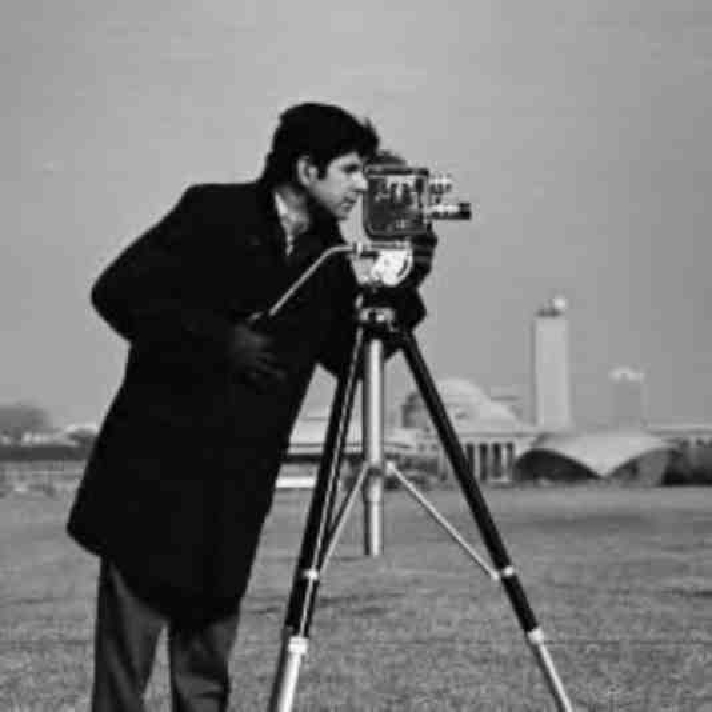
\includegraphics[width=8cm, height=8cm]{man-unmodified.jpg}
	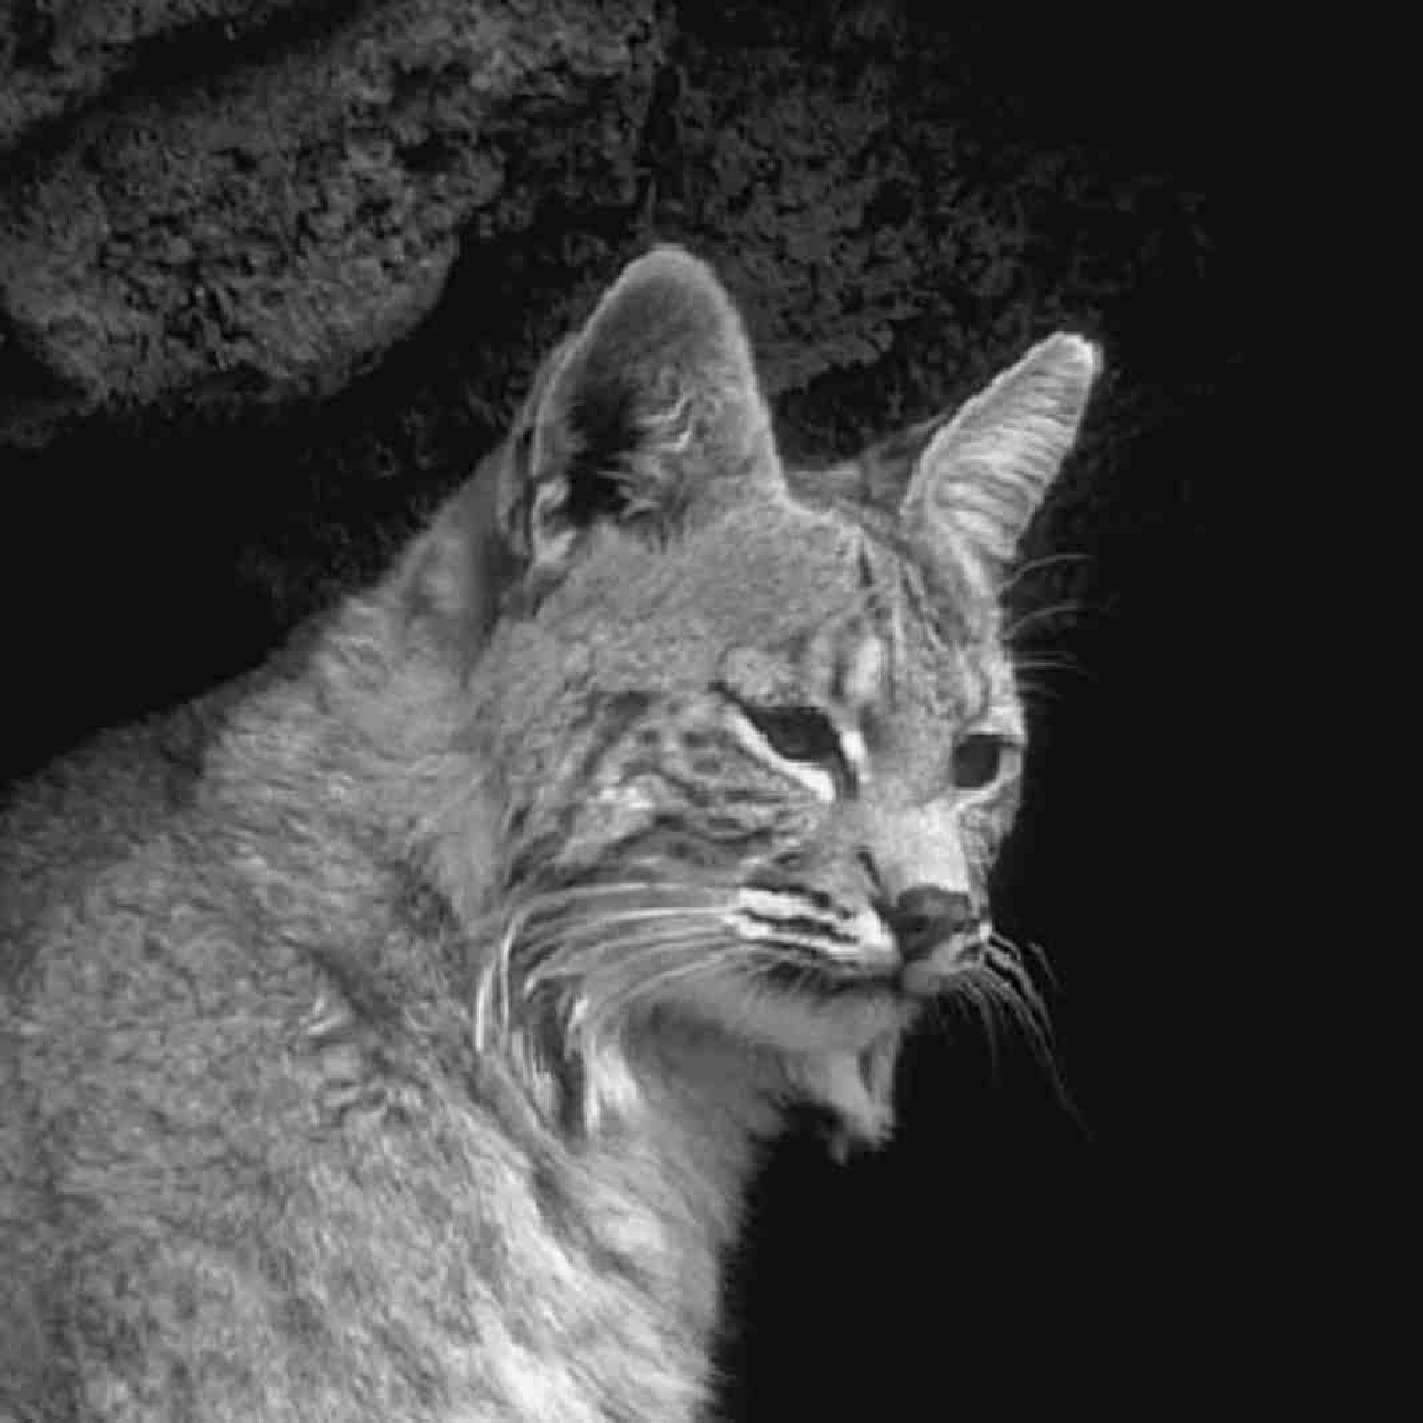
\includegraphics[width=8cm, height=8cm]{cat-unmodified.jpg}
\end{figure}
\begin{figure}
	\caption{Po uruchomieniem algorytmu (od lewej): obraz 1 (2133x2133, 300dpi), obraz 2 (2133x2133, 300dpi)}
	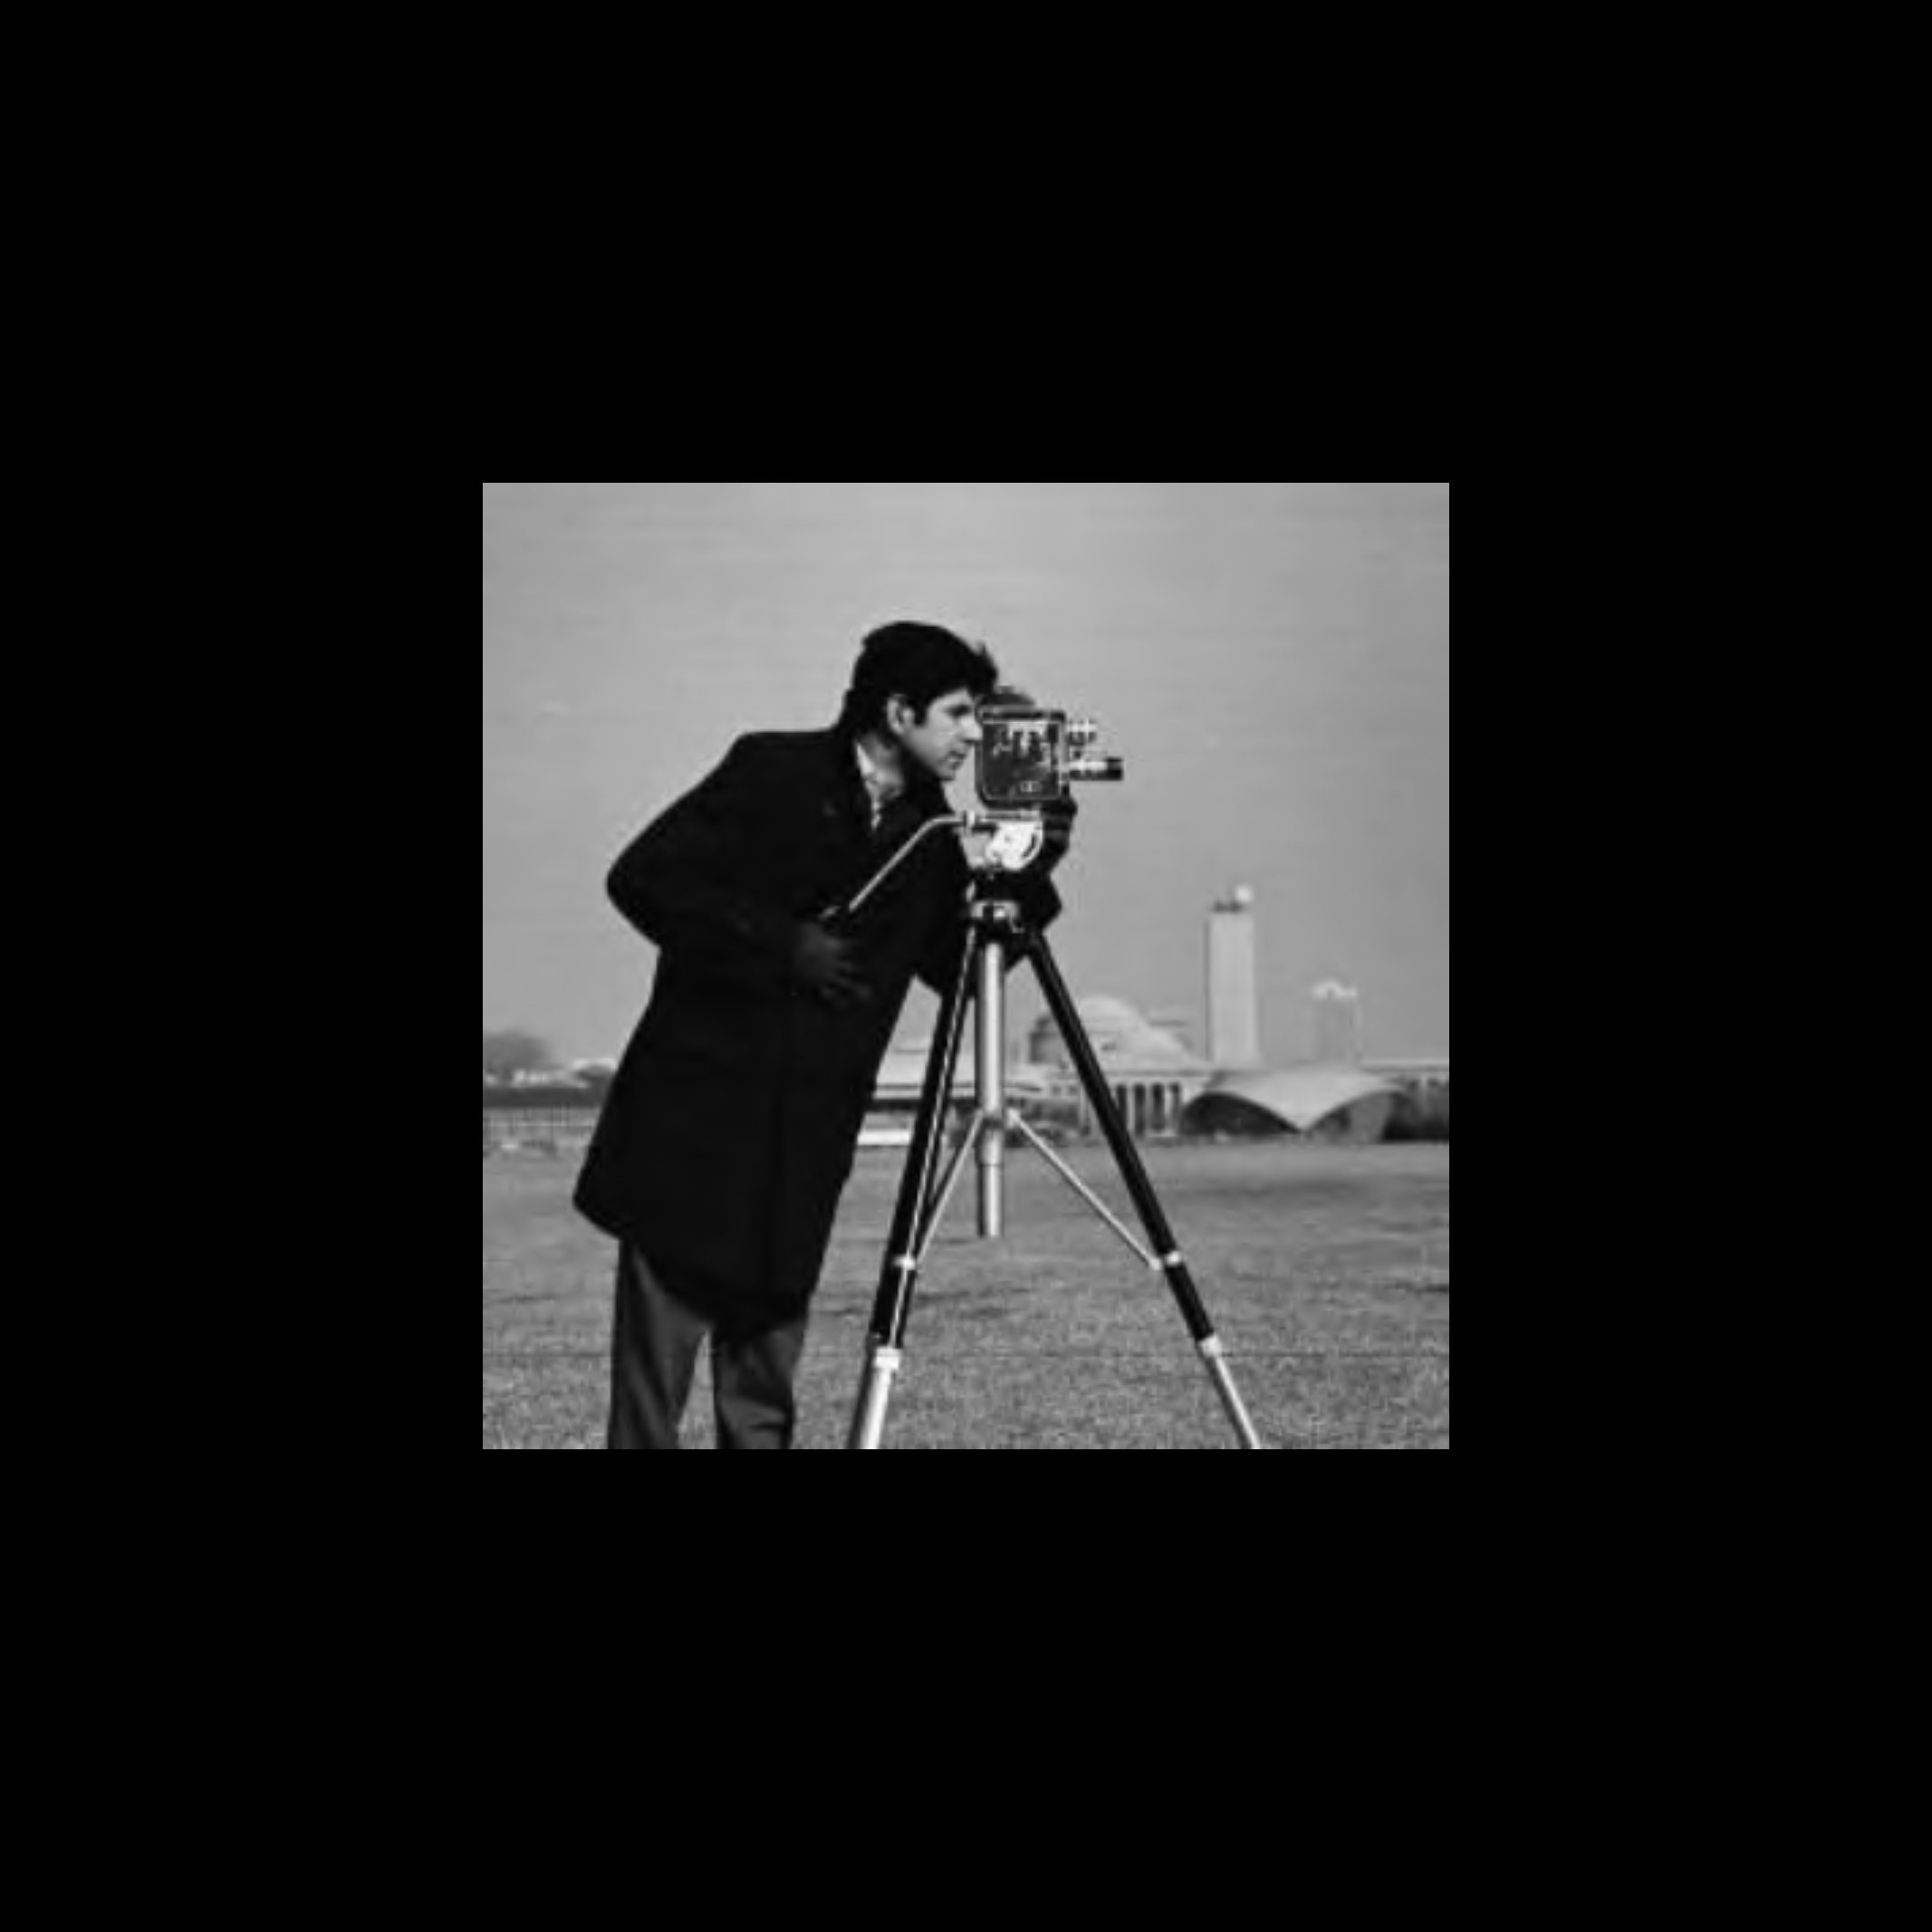
\includegraphics[width=8cm, height=8cm]{man-modified.png}
	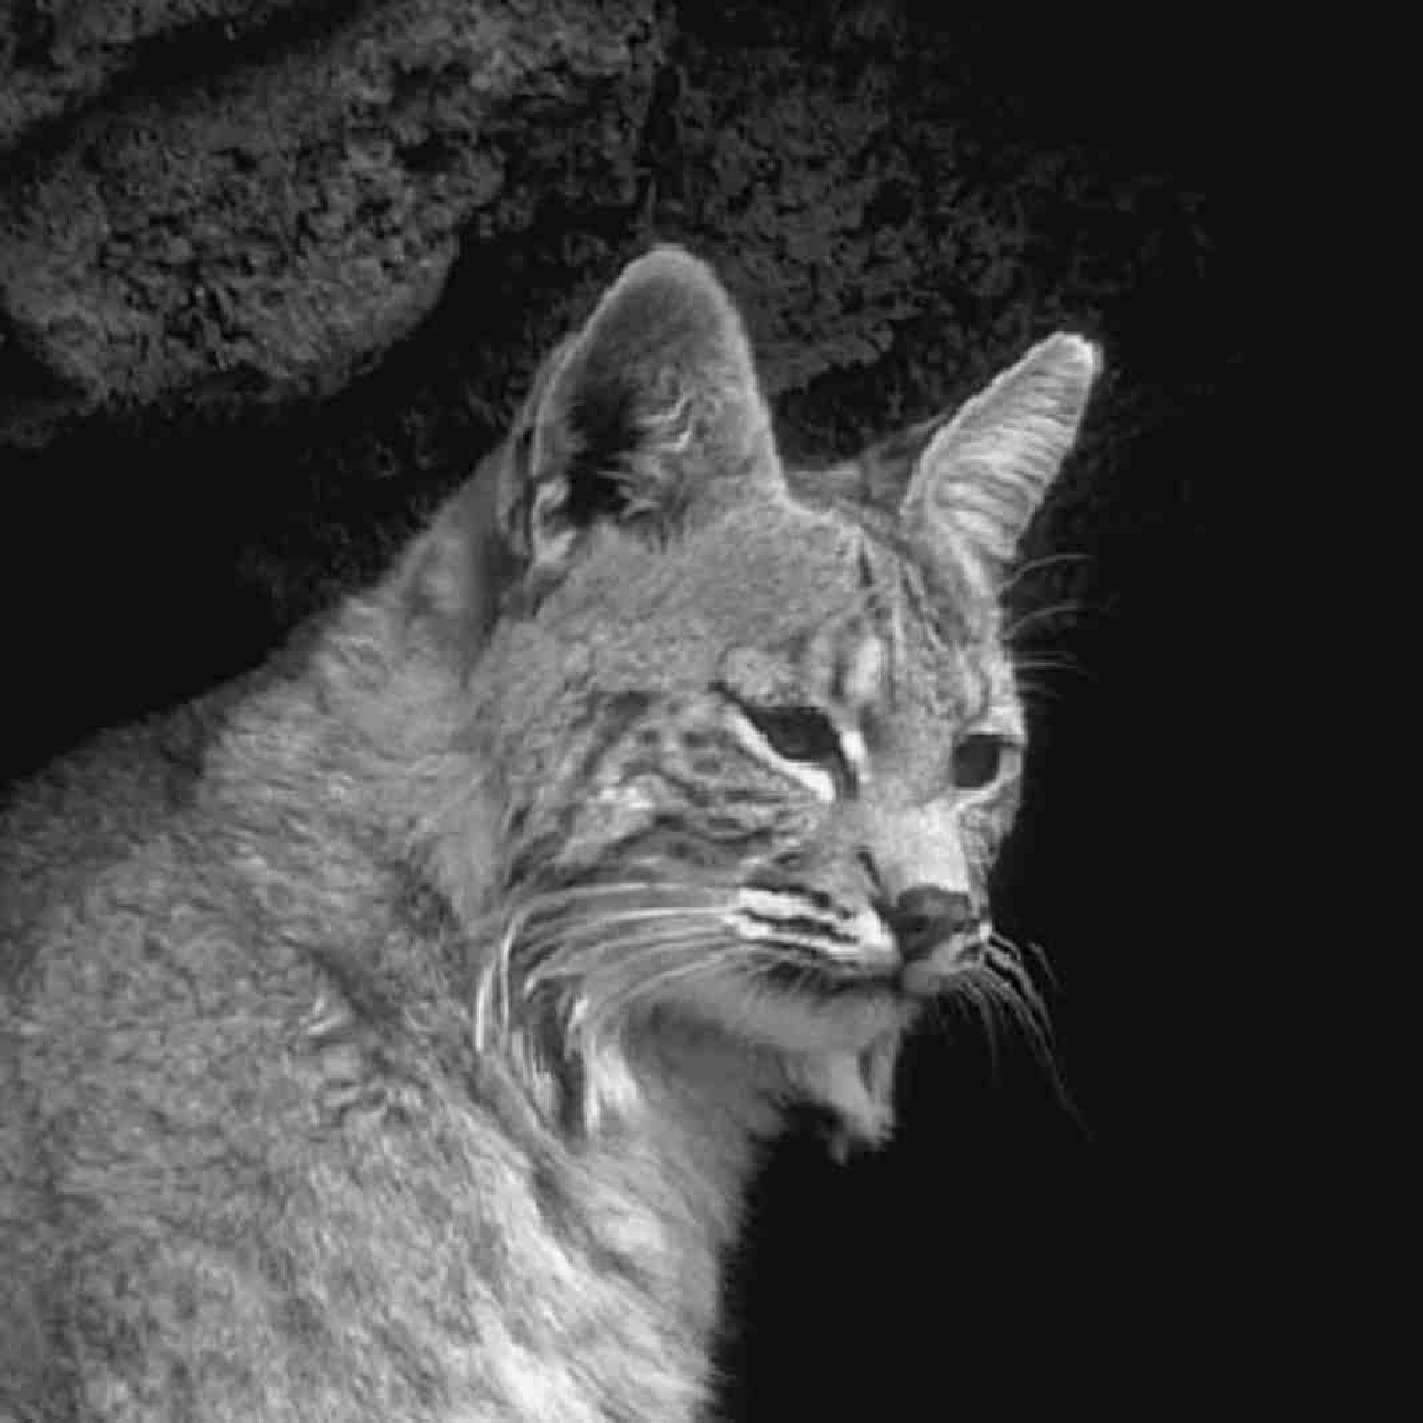
\includegraphics[width=8cm, height=8cm]{cat-unmodified.jpg}
\end{figure}
\subsection*{Kod źródłowy algorytmu}
\begin{python}
def geometricGray(self):
	print('geometric gray unificaiton start')
	width, height = self.firstDecoder.width, self.firstDecoder.height
	if width < self.maxWidth or height < self.maxHeight:
		# Create black background
		firstResult = numpy.zeros((self.maxHeight, self.maxWidth), numpy.uint8)
		# Copy smaller image to bigger
		startWidthIndex = int(round((self.maxWidth - width) / 2))
		startHeightIndex = int(round((self.maxHeight - height) / 2))
		pixelsBuffer = self.firstDecoder.getPixels()
		for h in range (0, height):
		for w in range (0, width):
		firstResult[h + startHeightIndex, w + startWidthIndex] = pixelsBuffer[h, w]
		img = Image.fromarray(firstResult, mode='L')
		img.save('Resources/ggUnification_1.png')
		print('first image done')
	
	width, height = self.secondDecoder.width, self.secondDecoder.height
	if width < self.maxWidth or height < self.maxHeight:
		# Create black background
		secondResult = numpy.zeros((self.maxHeight, self.maxWidth), numpy.uint8)
		# Copy smaller image to bigger
		startWidthIndex = int(round((self.maxWidth - width) / 2))
		startHeightIndex = int(round((self.maxHeight - height) / 2))
		pixelsBuffer = self.secondDecoder.getPixels()
		for h in range (0, height):
		for w in range (0, width):
		secondResult[h + startHeightIndex, w + startWidthIndex] = pixelsBuffer[h, w]
		img = Image.fromarray(secondResult, mode='L')
		img.save('Resources/ggUnification_2.png')
		print('second image done')
	print('geometric gray unification done')
\end{python}
\section{Ujednolicenie obrazów szarych rozdzielczościowe}
\subsection*{Algorytm}
\subsubsection*{Opis}
Po użyciu ujednolicenia geometrycznego można użyć ujednolicenia rozdzielczościowego, które przeskaluje obraz z mniejszej postaci do większej dzięki czemu nie zostanie nam czarna ramka wokół obrazu. Wynikiem będzie większy obraz niż początkowo bez czarnego obwodu wokół. 
Mniejszy obraz można przeskalować do większych wymiarów przenosząc wszystkie piksele z uwzględnieniem luk pomiędzy nimi i następnie użycia interpolacji do zamazania tych luk. 
Interpolacja działa na zasadzie pobierania wartości z okolicznych pikseli i wyciągania z nich średniej, która posłuży jako baza koloru dla nowego piksela. 
\subsubsection*{Kroki}
\begin{enumerate}
	\item Ustalenie nowych wymiarów obrazu
	\item Obliczenie odległości pomiędzy pikselami (\textit{scaleFactoryH, scaleFactoryW})
	\item Naniesienie pikseli z mniejszego obrazu na większy z uwzględnieniem luk
	\item Interpolacja
\end{enumerate}
\begin{figure}
	\caption{Skutki braku interpolacji}
	\begin{center}
		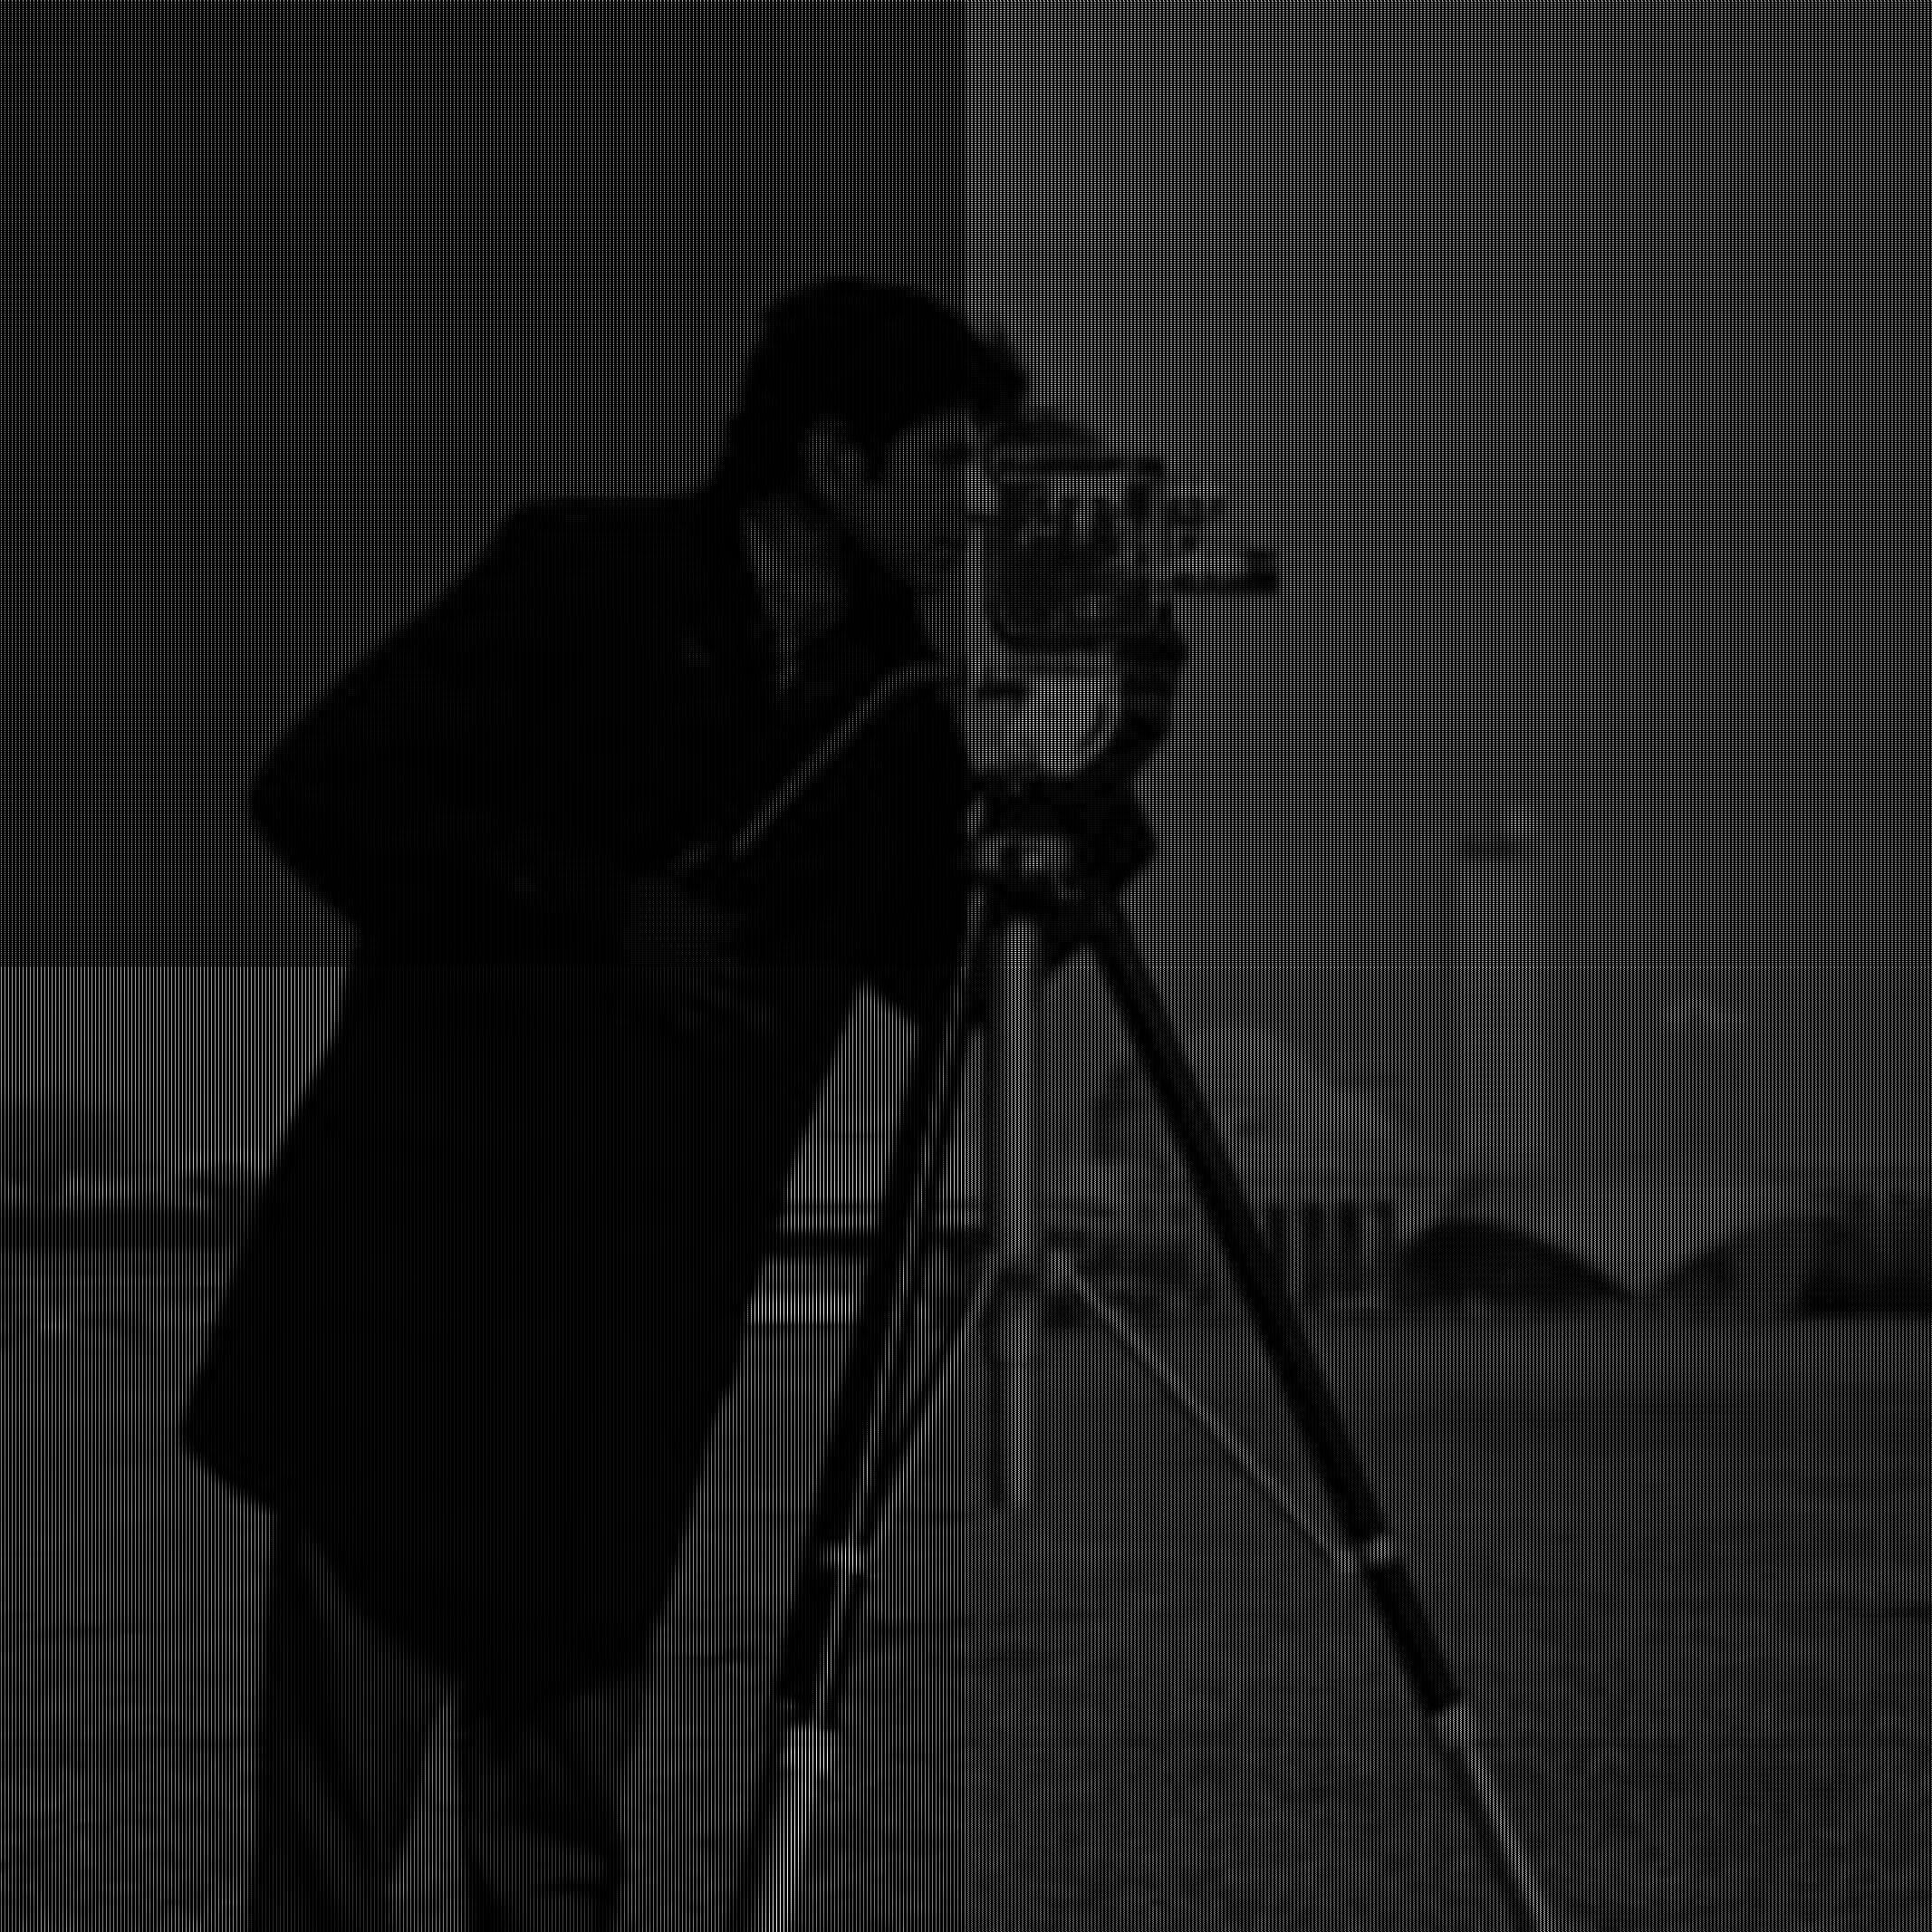
\includegraphics[width=8cm, height=8cm]{man-without-interpolation.png}
	\end{center}
\end{figure}
\begin{figure}
	\caption{Przed uruchomieniem algorytmu (od lewej): obraz 1 (2133x2133, 300dpi), obraz 2 (2133x2133, 300dpi)}
	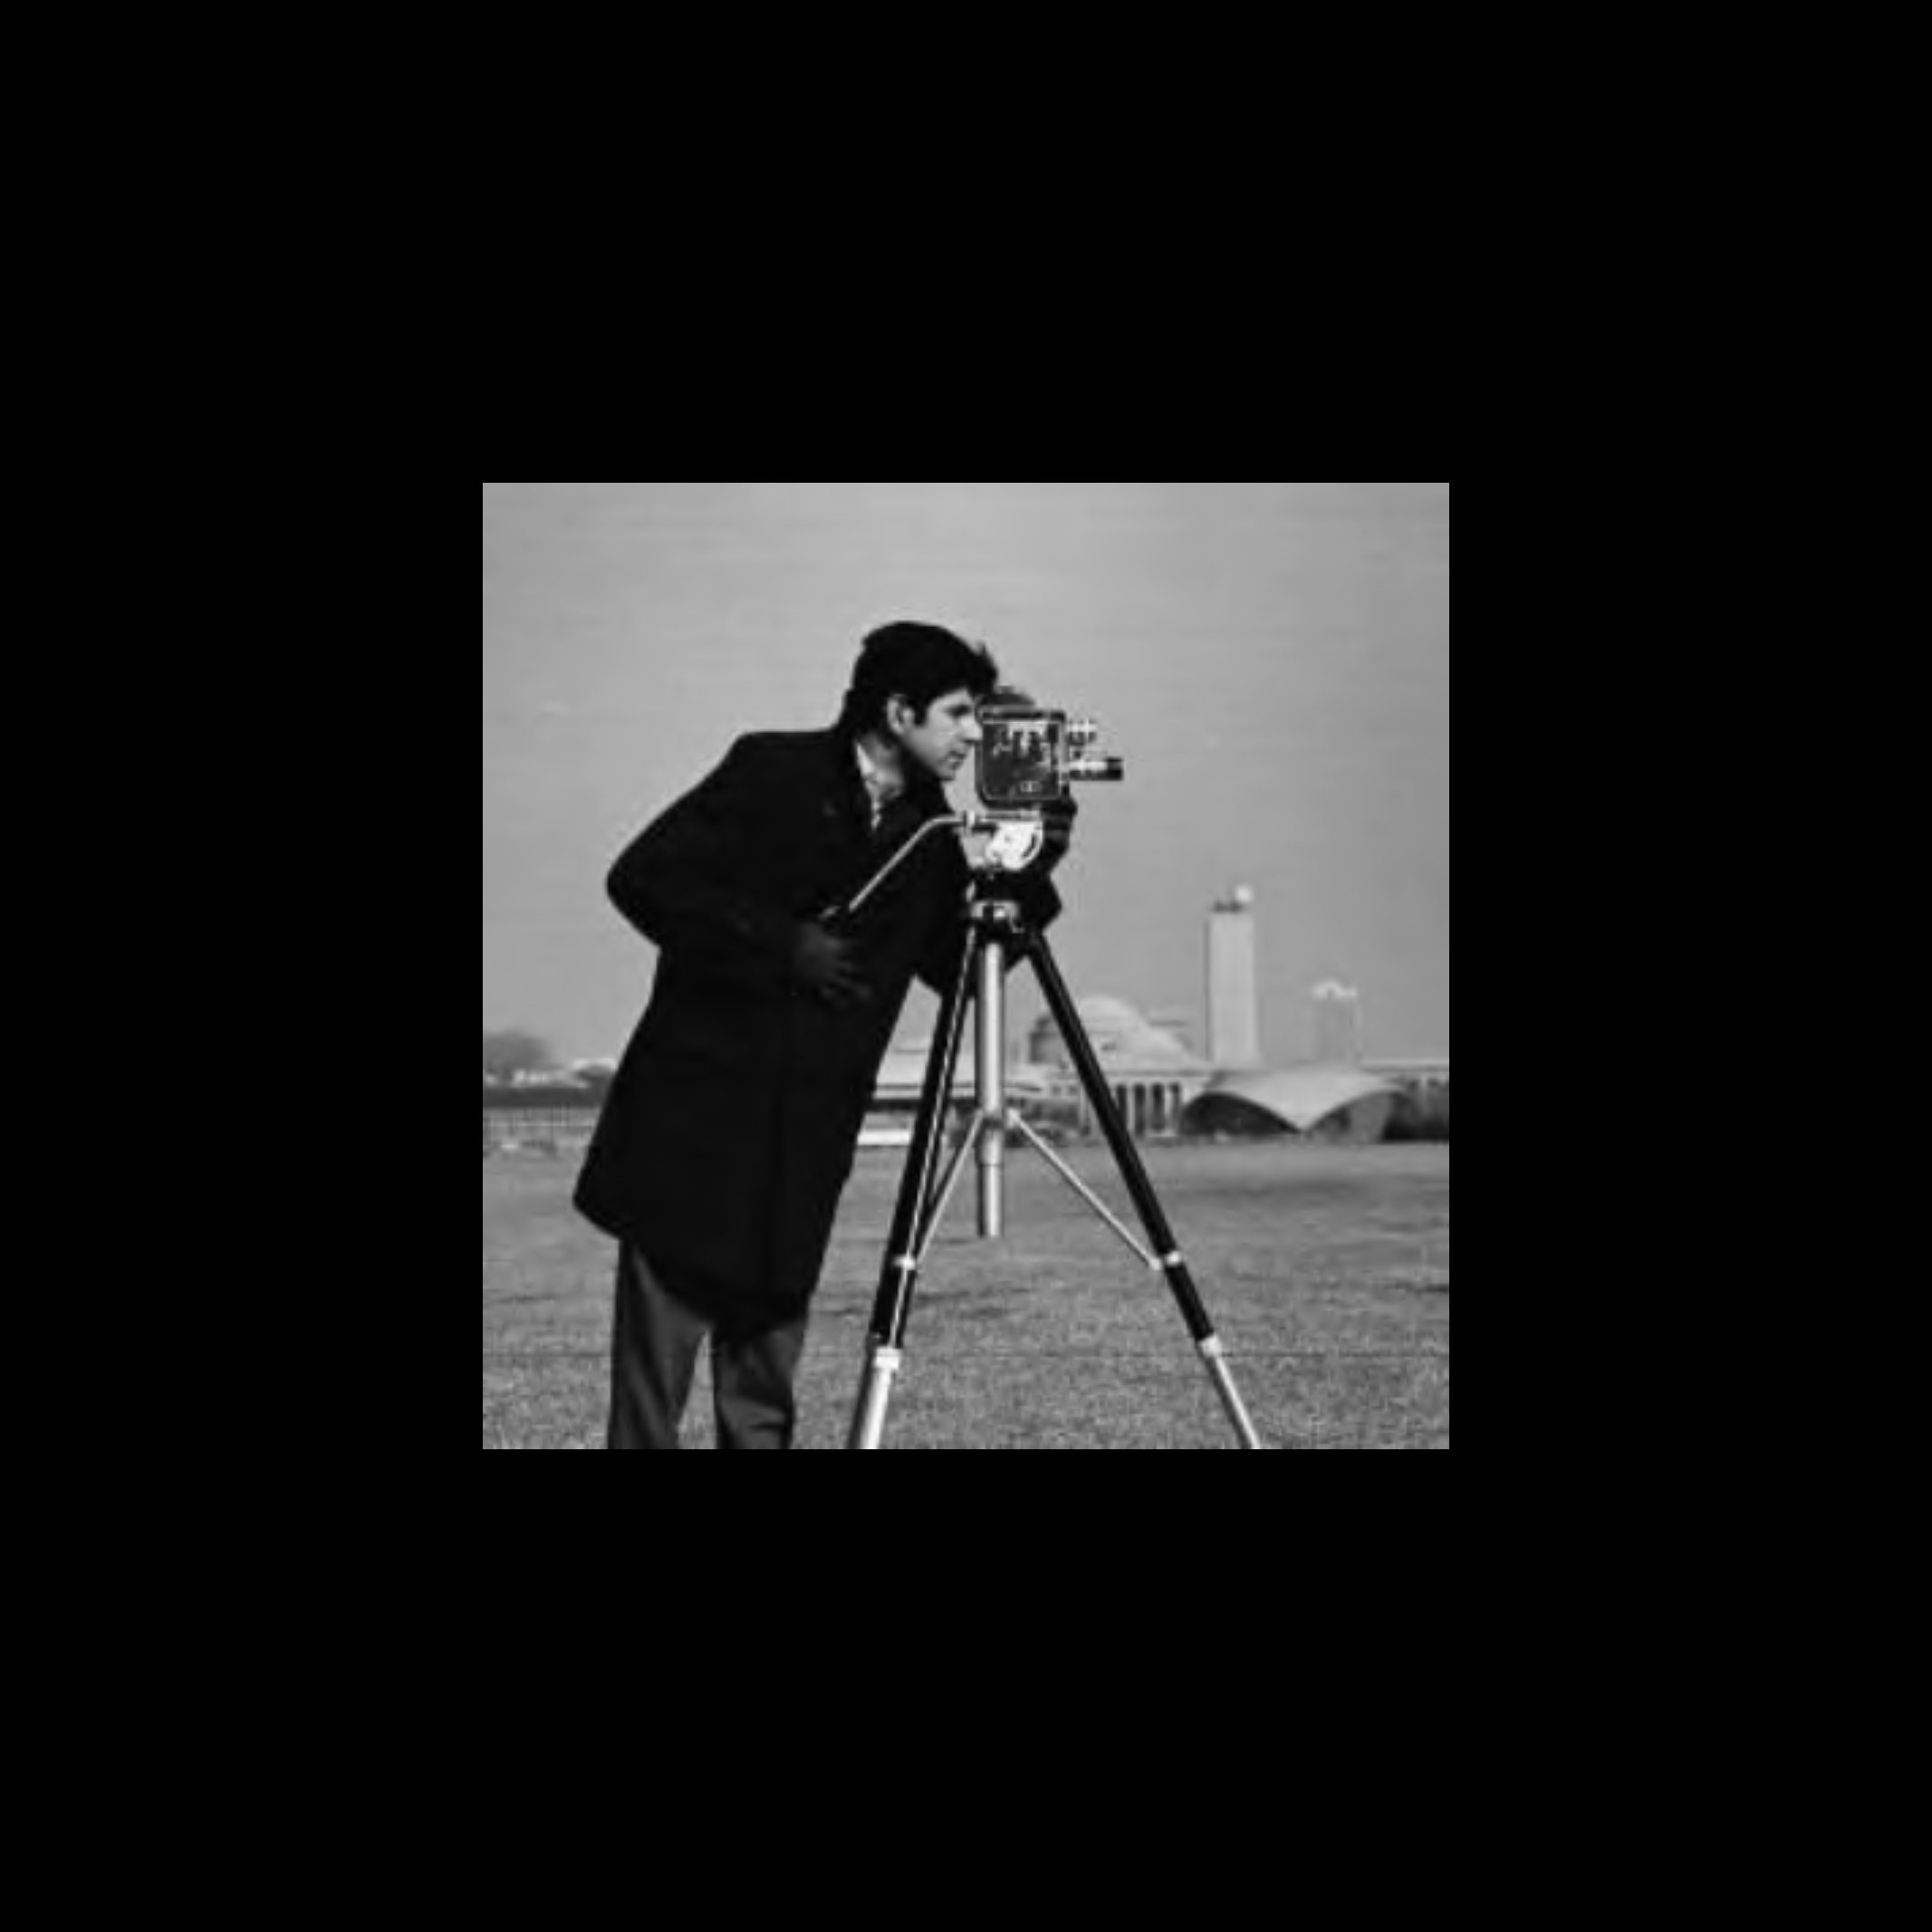
\includegraphics[width=8cm, height=8cm]{man-modified.png}
	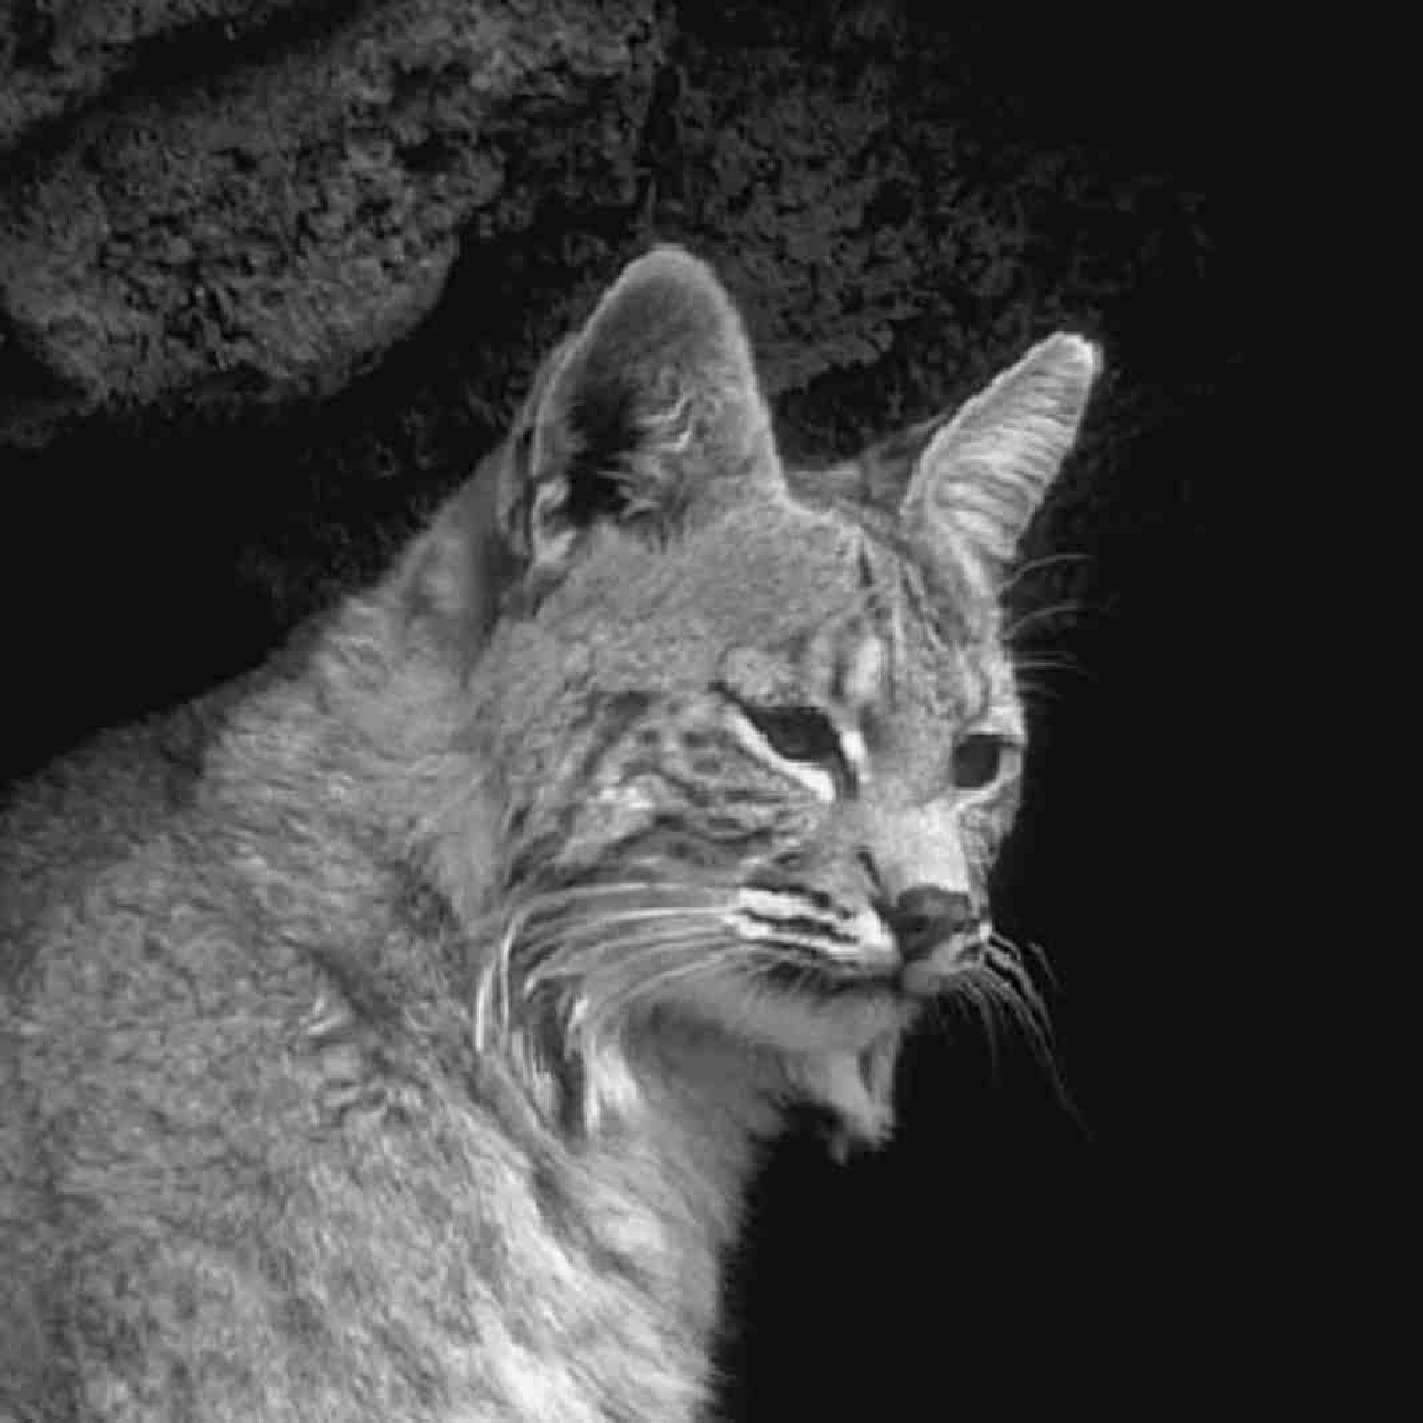
\includegraphics[width=8cm, height=8cm]{cat-unmodified.jpg}
\end{figure}
\begin{figure}
	\caption{Po uruchomieniem algorytmu (od lewej): obraz 1 (2133x2133, 300dpi), obraz 2 (2133x2133, 300dpi)}
	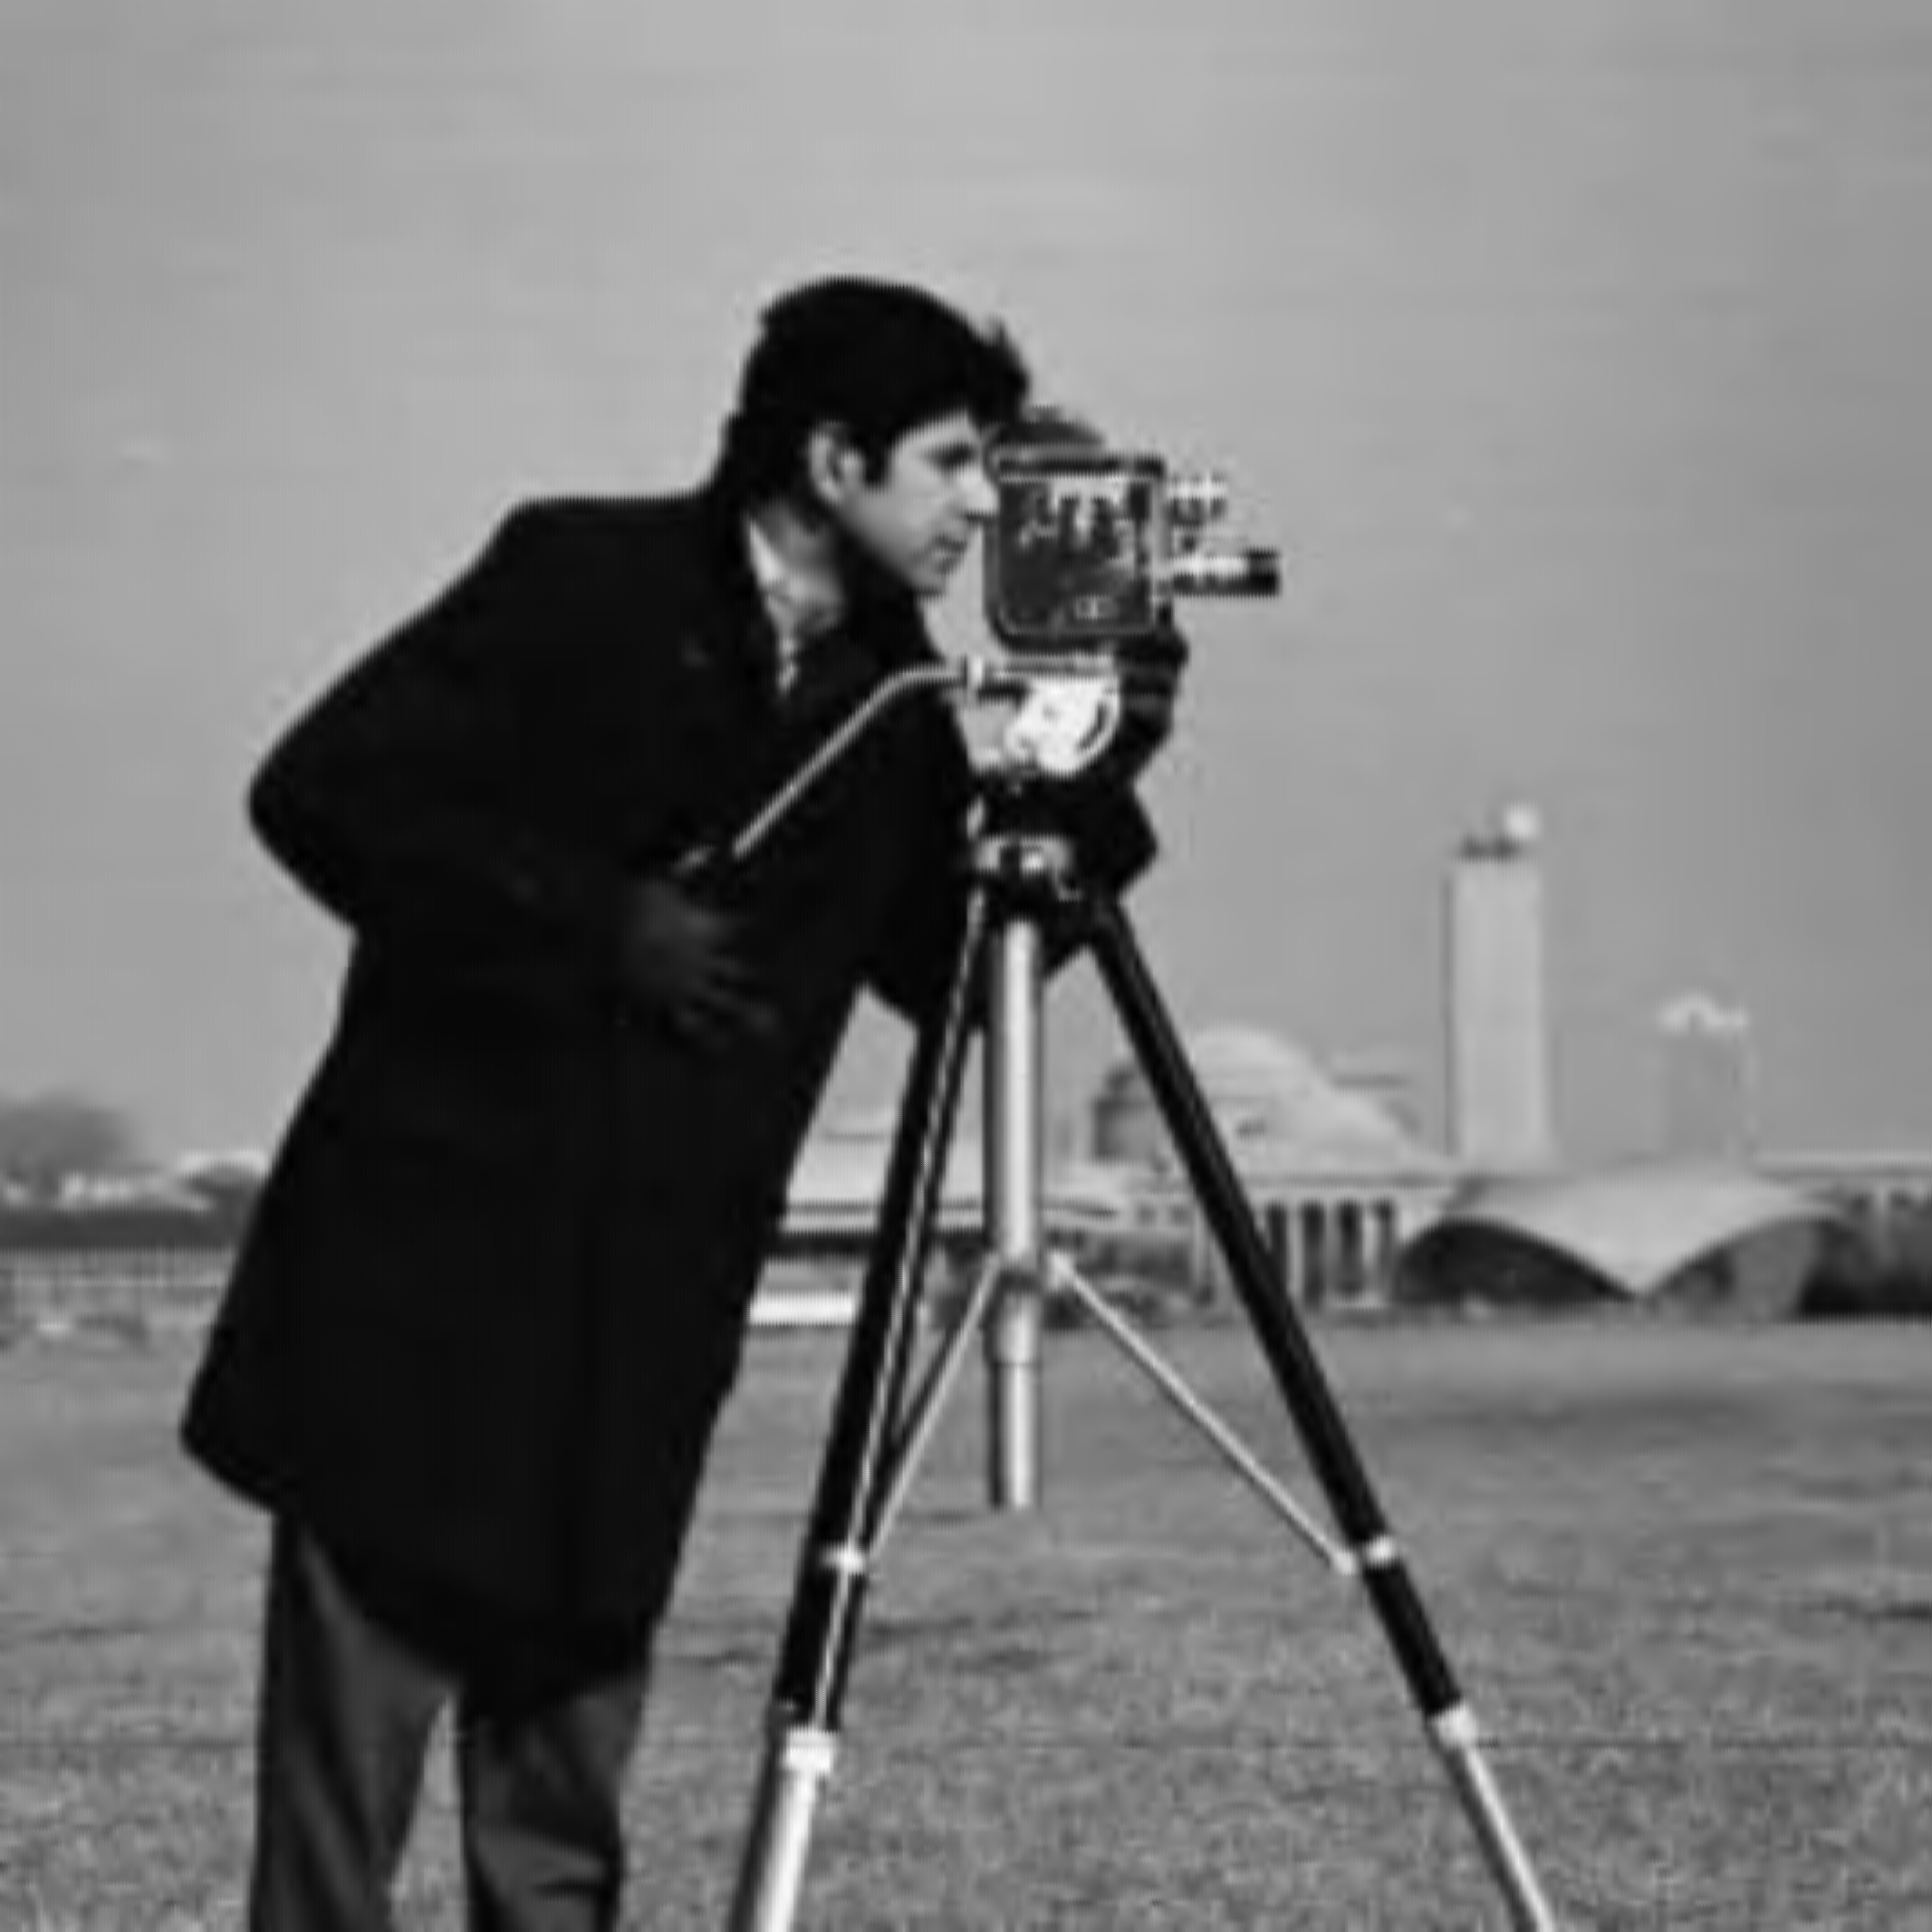
\includegraphics[width=8cm, height=8cm]{man-rastar-unification.png}
	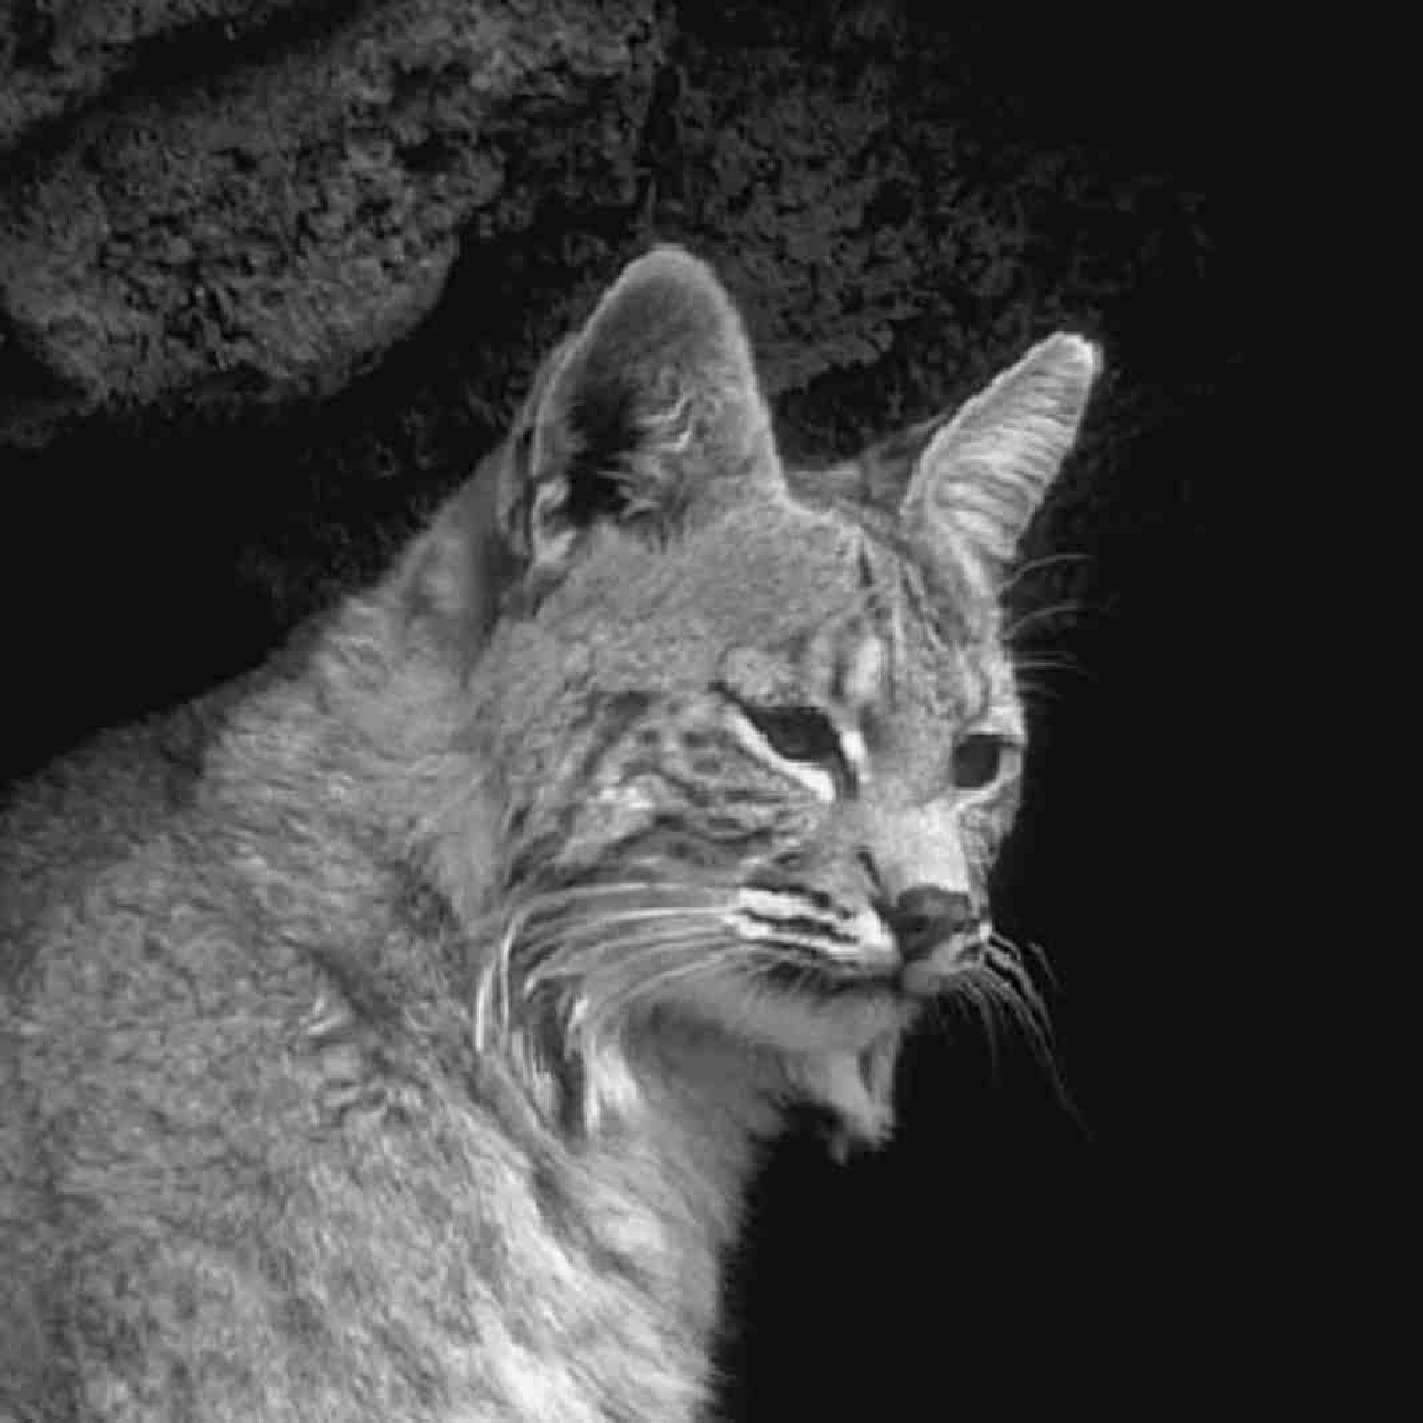
\includegraphics[width=8cm, height=8cm]{cat-unmodified.jpg}
\end{figure}
\subsection*{Kod źródłowy algorytmu}
\begin{python}
def rasterGray(self):
	print('raster gray unification start')
	self._scaleUpGray(self.firstDecoder, 'Resources/rgUnification_1.png')
	print('first image done')
	self._scaleUpGray(self.secondDecoder, 'Resources/rgUnification_2.png')
	print('second image done')
	print('raster gray unification done')

def _scaleUpGray(self, decoder, outputPath):
	width, height = decoder.width, decoder.height
	scaleFactoryW = float(self.maxWidth) / width
	scaleFactoryH = float(self.maxHeight) / height
	if width < self.maxWidth or height < self.maxHeight:
		pixelsBuffer = decoder.getPixels()
		result = numpy.zeros((self.maxHeight, self.maxWidth), numpy.uint8)
		# Fill values
		for h in range(height):
			for w in range(width):
				if w%2 == 0:
					result[int(scaleFactoryH * h), int(round(scaleFactoryW * w)) + 1] = pixelsBuffer[h, w]
				if w%2 == 1:
					result[int(round(scaleFactoryH * h)) + 1, int(scaleFactoryW * w)] = pixelsBuffer[h, w]
		# Interpolate
		self._interpolateGray(result)
		img = Image.fromarray(result, mode='L')
		img.save(outputPath)

def _interpolateGray(self, result):
	for h in range(self.maxHeight):
		for w in range(self.maxWidth):
			value = 0
			count = 0
			if result[h, w] == 0:
				for hOff in range(-1, 2):
					for wOff in range(-1, 2):
						hSafe = h if ((h + hOff) > (self.maxHeight - 2)) | ((h + hOff) < 0) else (h + hOff)
						wSafe = w if ((w + wOff) > (self.maxWidth - 2)) | ((w + wOff) < 0) else (w + wOff)
						if result[hSafe, wSafe] != 0:
							value += result[hSafe, wSafe]
							count += 1
				result[h, w] = value / count
\end{python}
\section{Ujednolicenie obrazów RGB geometryczne}
\subsection*{Algorytm}
\subsubsection*{Opis}
Algorytm geometrycznego ujednolicenia obrazów ma za zadanie sprowadzić oba obrazy do tej samej liczby pikseli w każdym wierszu i każdej kolumnie. 
Różnica pomiędzy tym przypadkiem a szarym sprawia, że ważne jest użycie odpowiednich struktur danych w taki sposób aby każdy z kanałów RGB był w stanie się pomieścić. Niewątpliwie ważne jest struktura danych uwzględniała kolejność w jakim kolory są przechowywane, inaczej może dojść do sytuacji w której nie dostaniemy oczekiwanego rezultatu. 
\subsubsection*{Kroki}
\begin{enumerate}
	\item Porównaj szerokości i wysokości obu obrazów i wybierz największe. 
	\item Jeśli pierwszy lub drugi obraz mają szerokość lub wysokość mniejszą od największej dostępnej to:
	\begin{enumerate}
		\item Utwórz czarne tło
		\item Przenieś z wyśrodkowaniem piksle na czarne tło z uwzględnieniem każdego z kanałów RGB
	\end{enumerate}
	\item Jeśli żaden z warunków jest niespełniony to nie rób nic
\end{enumerate}
\begin{figure}
	\caption{Przed uruchomieniem algorytmu (od lewej): obraz 1 (512x512, 300dpi), obraz 2 (1024x1024, 300dpi)}
	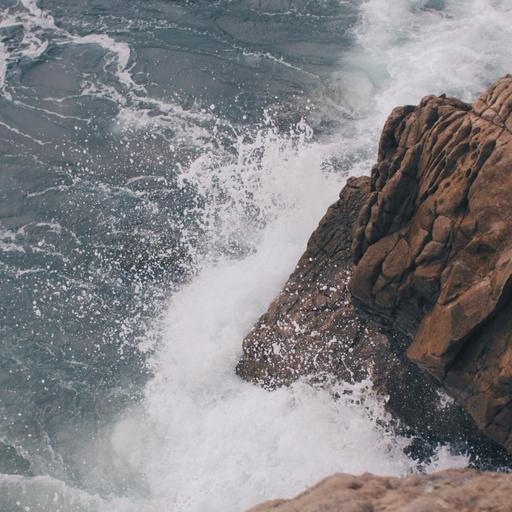
\includegraphics[width=8cm, height=8cm]{sea-unmodified.jpg}
	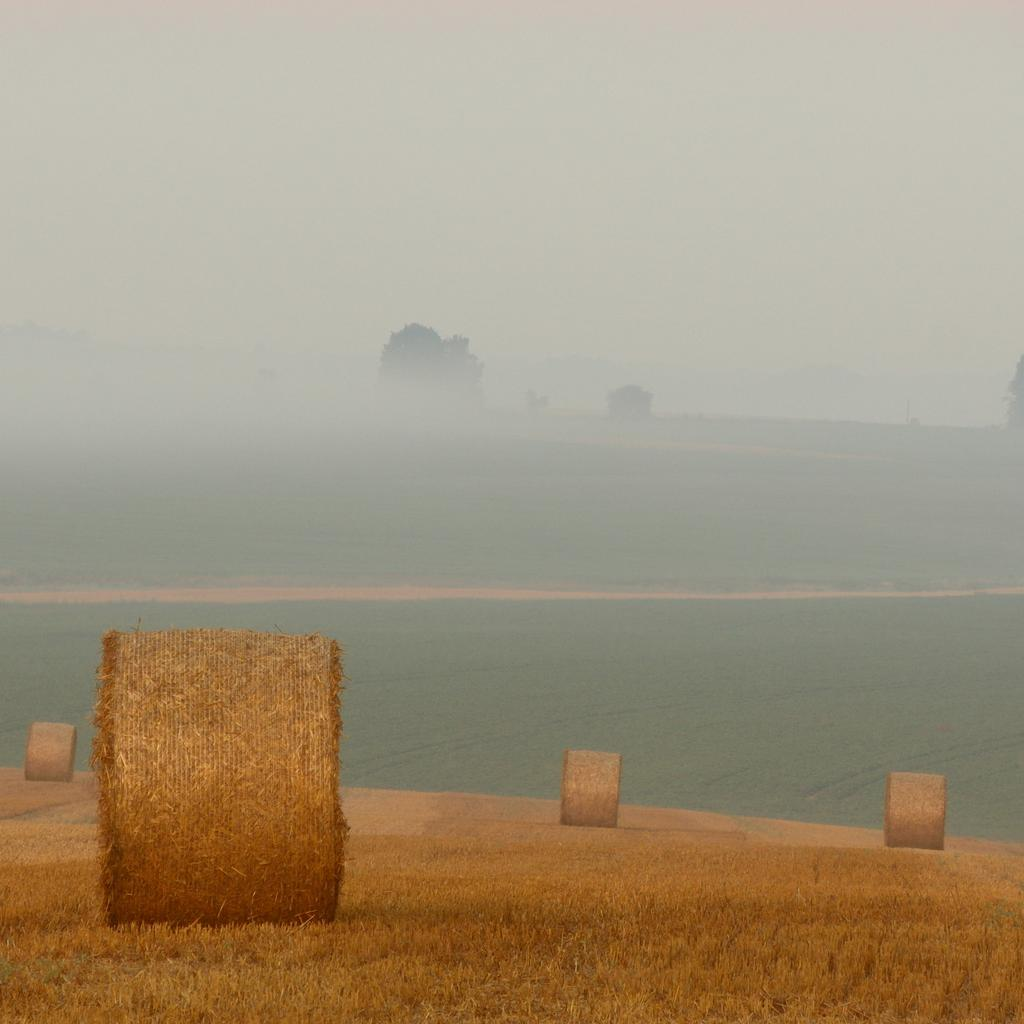
\includegraphics[width=8cm, height=8cm]{field-unmodified.jpg}
\end{figure}
\begin{figure}
	\caption{Po uruchomieniem algorytmu (od lewej): obraz 1 (1024x1024, 300dpi), obraz 2 (1024x1024, 300dpi)}
	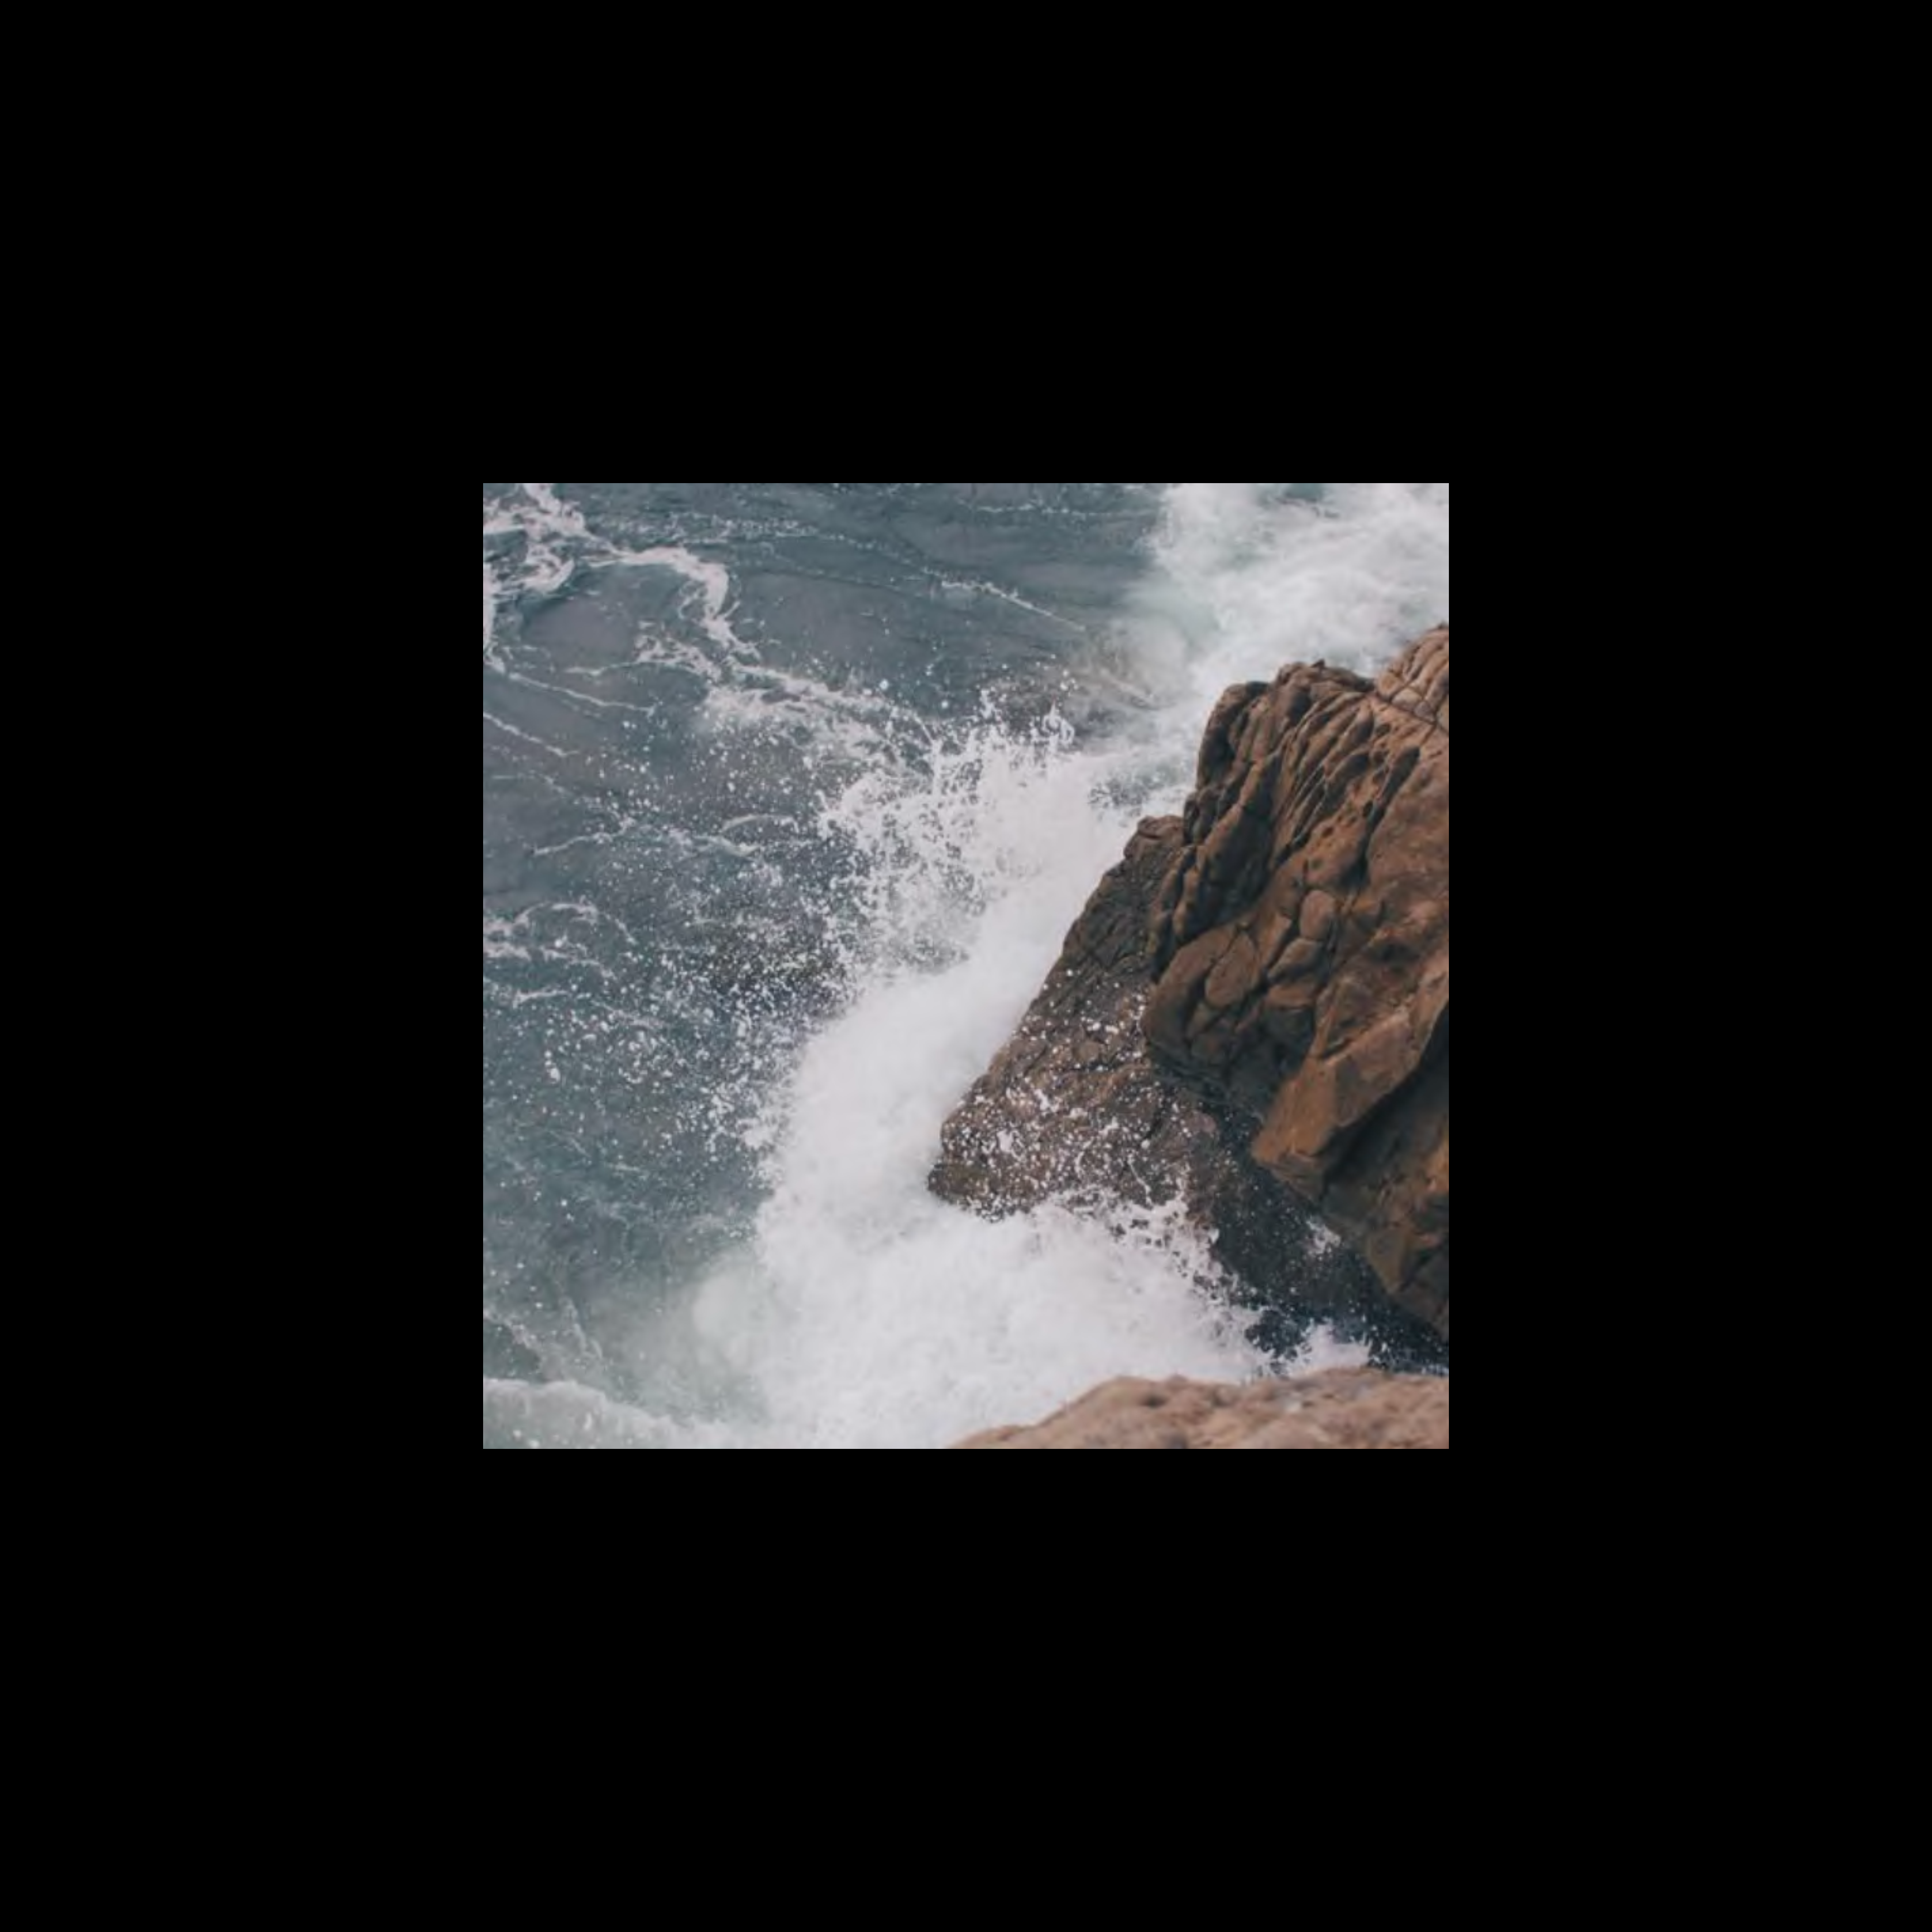
\includegraphics[width=8cm, height=8cm]{sea-geo-modified.png}
	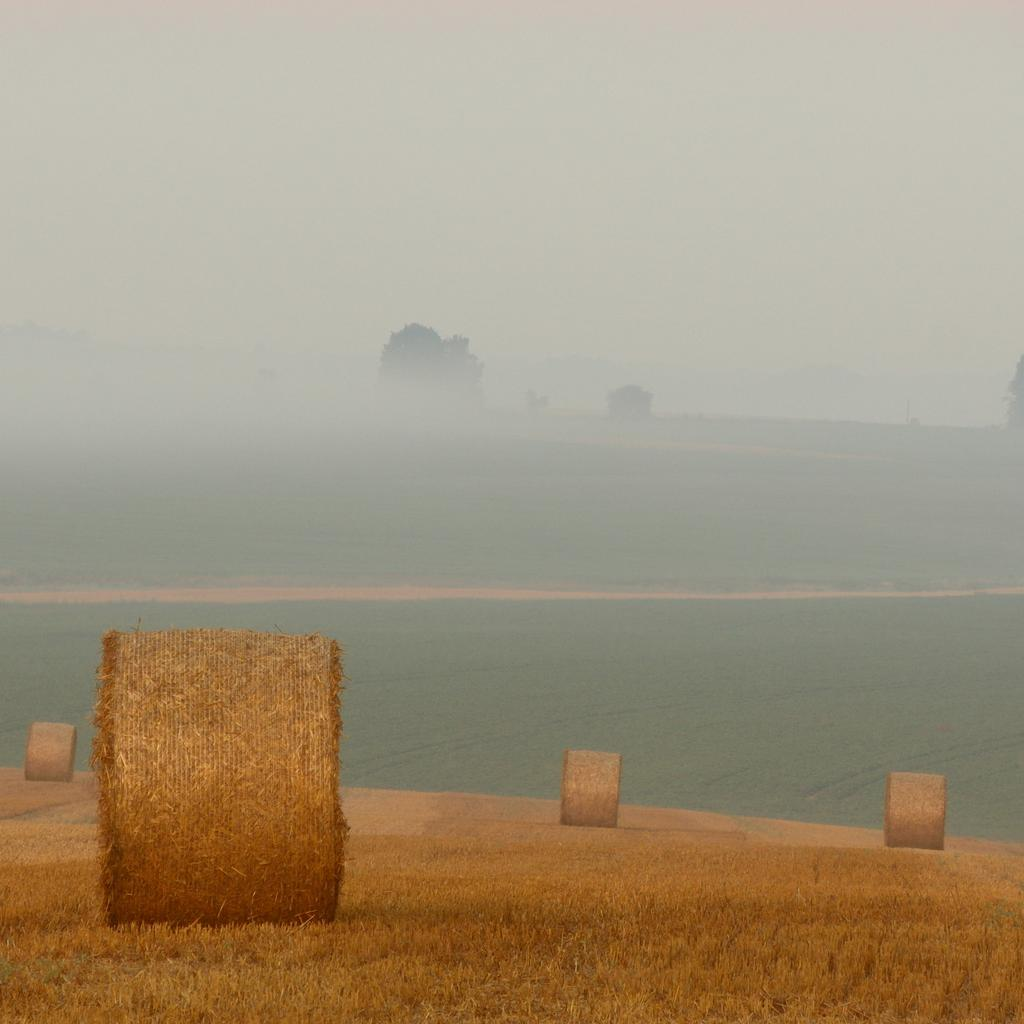
\includegraphics[width=8cm, height=8cm]{field-unmodified.jpg}
\end{figure}
\begin{figure}
	\caption{Przed uruchomieniem algorytmu (od lewej): obraz 3 (126x126, 300dpi), obraz 4 (256x256, 300dpi)}
	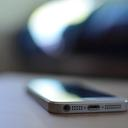
\includegraphics[width=8cm, height=8cm]{phone-unmodified.jpg}
	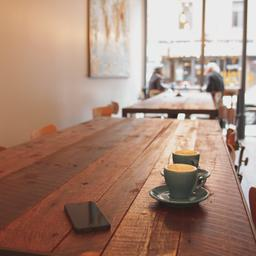
\includegraphics[width=8cm, height=8cm]{coffee-unmodified.jpg}
\end{figure}
\begin{figure}
	\caption{Po uruchomieniem algorytmu (od lewej): obraz 3 (126x126, 300dpi), obraz 4 (256x256, 300dpi)}
	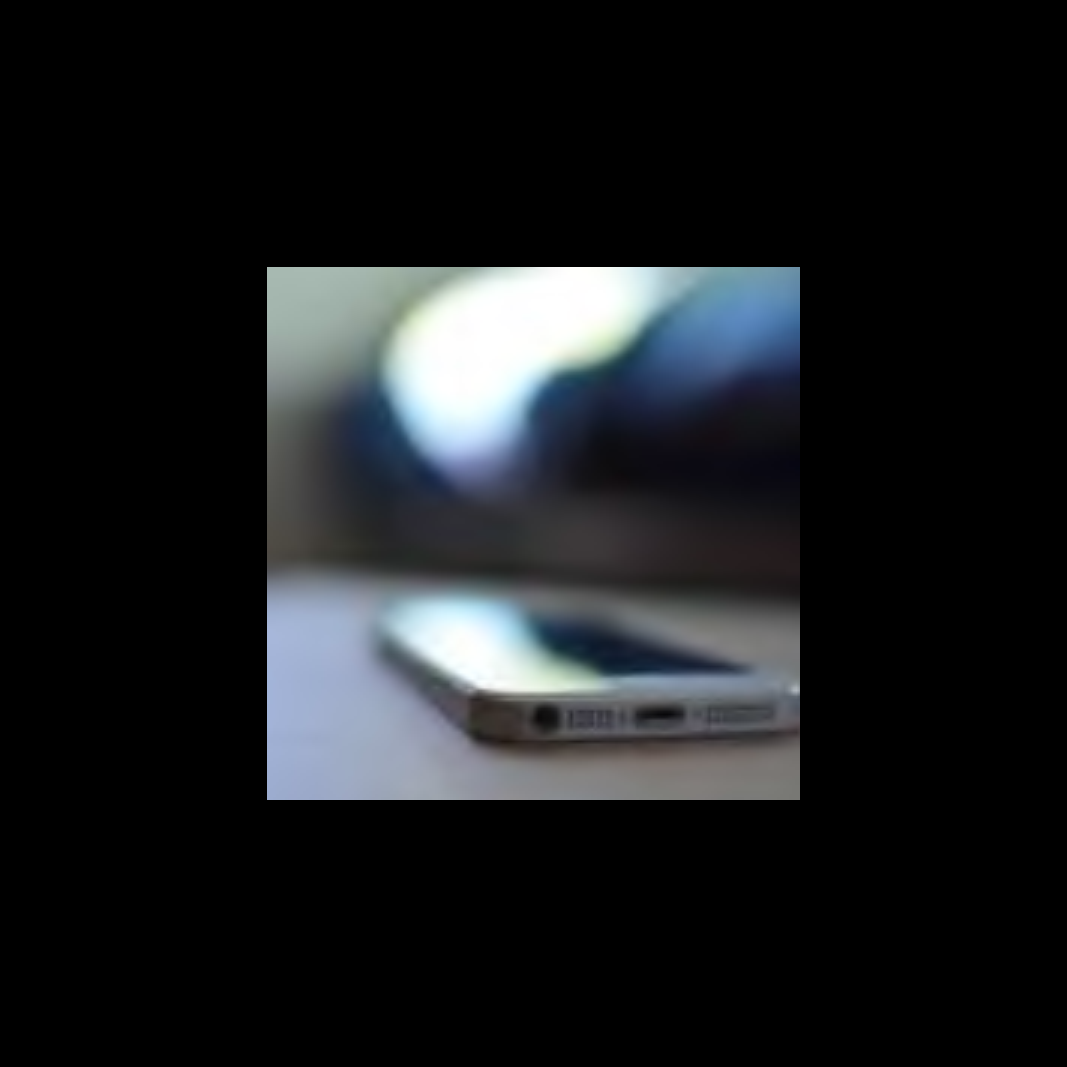
\includegraphics[width=8cm, height=8cm]{phone-geo-modified.png}
	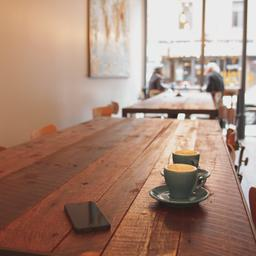
\includegraphics[width=8cm, height=8cm]{coffee-unmodified.jpg}
\end{figure}
\newpage
\subsection*{Kod źródłowy algorytmu}
\begin{python}
def geometricColor(self):
	print('geometric color unificaiton start')
	self.firstDecoder.setColor()
	width, height = self.firstDecoder.width, self.firstDecoder.height
	if width < self.maxWidth or height < self.maxHeight:
		result = self._paintInMiddleColor(self.firstDecoder)
		img = Image.fromarray(result, 'RGB')
		img.save('Resources/gcUnification_1.png')
		print('first image done')
	
	self.secondDecoder.setColor()
	width, height = self.secondDecoder.width, self.secondDecoder.height
	if width < self.maxWidth or height < self.maxHeight:
		result = self._paintInMiddleColor(self.secondDecoder)
		img = Image.fromarray(result, 'RGB')
		img.save('Resources/gcUnification_2.png')
		print('second image done')
	print('geometric color unification done')
	
def _paintInMiddleColor(self, decoder):
	# Create black background
	result = numpy.full((self.maxHeight, self.maxWidth, 3), 0, numpy.uint8)
	# Copy smaller image to bigger
	width, height = decoder.width, decoder.height
	startWidthIndex = int(round((self.maxWidth - width) / 2))
	startHeightIndex = int(round((self.maxHeight - height) / 2))
	pixelsBuffer = decoder.getPixels24Bits()
	for h in range (0, height):
		for w in range (0, width):
			result[h + startHeightIndex, w + startWidthIndex] = pixelsBuffer[h, w]
	return result
\end{python}
\section{Ujednolicenie obrazów RGB rozdzielczościowe}
\subsection*{Algorytm}
\subsubsection*{Opis}
Po użyciu ujednolicenia geometrycznego można użyć ujednolicenia rozdzielczościowego, które przeskaluje obraz z mniejszej postaci do większej dzięki czemu nie zostanie nam czarna ramka wokół obrazu. Wynikiem będzie większy obraz niż początkowo bez czarnego obwodu wokół. 
Mniejszy obraz można przeskalować do większych wymiarów przenosząc wszystkie piksele z uwzględnieniem luk pomiędzy nimi i następnie użycia interpolacji do zamazania tych luk. 
Interpolacja działa na zasadzie pobierania wartości z okolicznych pikseli i wyciągania z nich średniej, która posłuży jako baza koloru dla nowego piksela. 
\subsubsection*{Kroki}
\begin{enumerate}
	\item Ustalenie nowych wymiarów obrazu
	\item Obliczenie odległości pomiędzy pikselami (\textit{scaleFactoryH, scaleFactoryW})
	\item Naniesienie pikseli z mniejszego obrazu na większy z uwzględnieniem luk
	\item Interpolacja
\end{enumerate}
\begin{figure}
	\caption{Skutki braku interpolacji}
	\begin{center}
		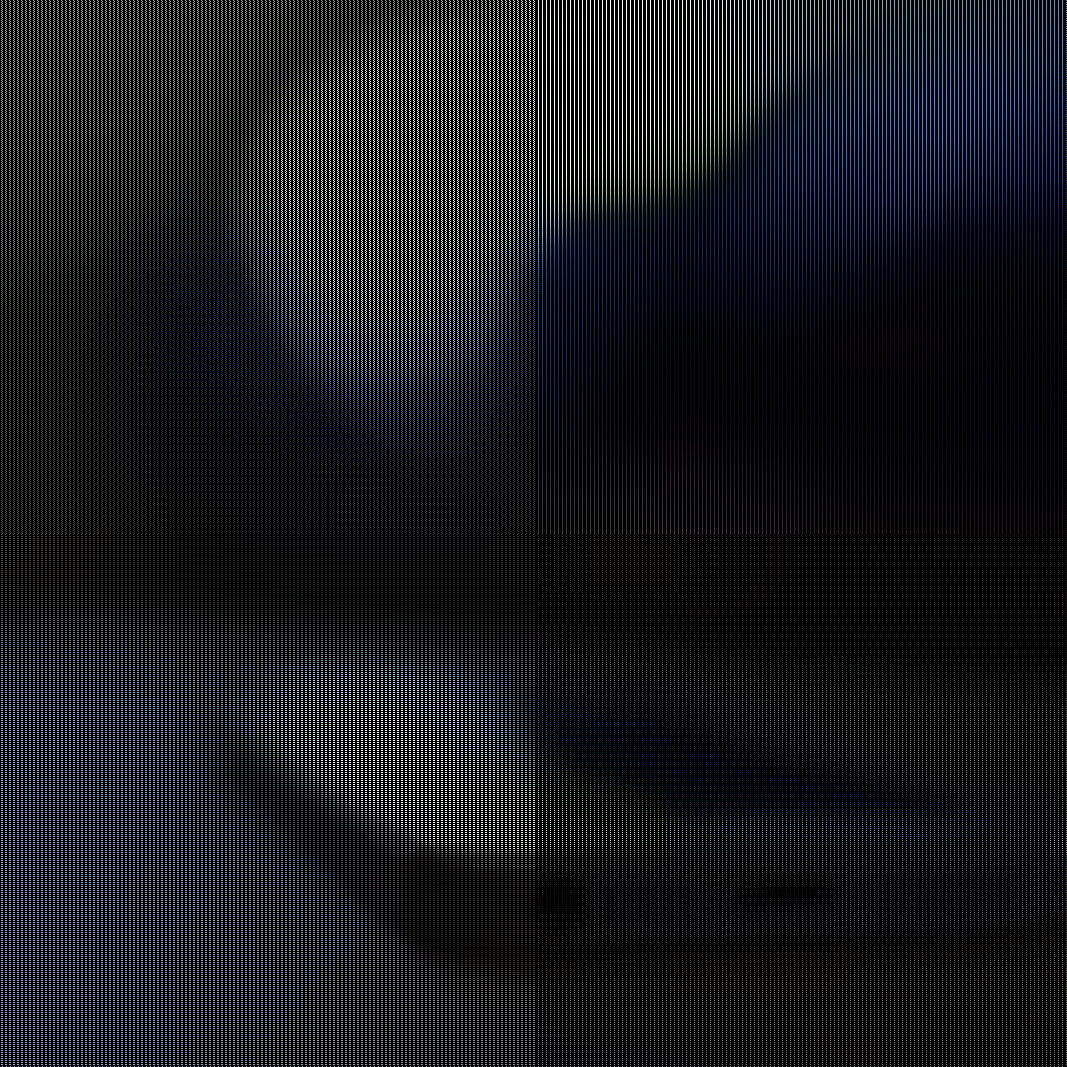
\includegraphics[width=8cm, height=8cm]{phone-without-interpolation.png}
	\end{center}
\end{figure}
\begin{figure}
	\caption{Przed uruchomieniem algorytmu (od lewej): obraz 1 (256x256, 300dpi), obraz 2 (256x256, 300dpi)}
	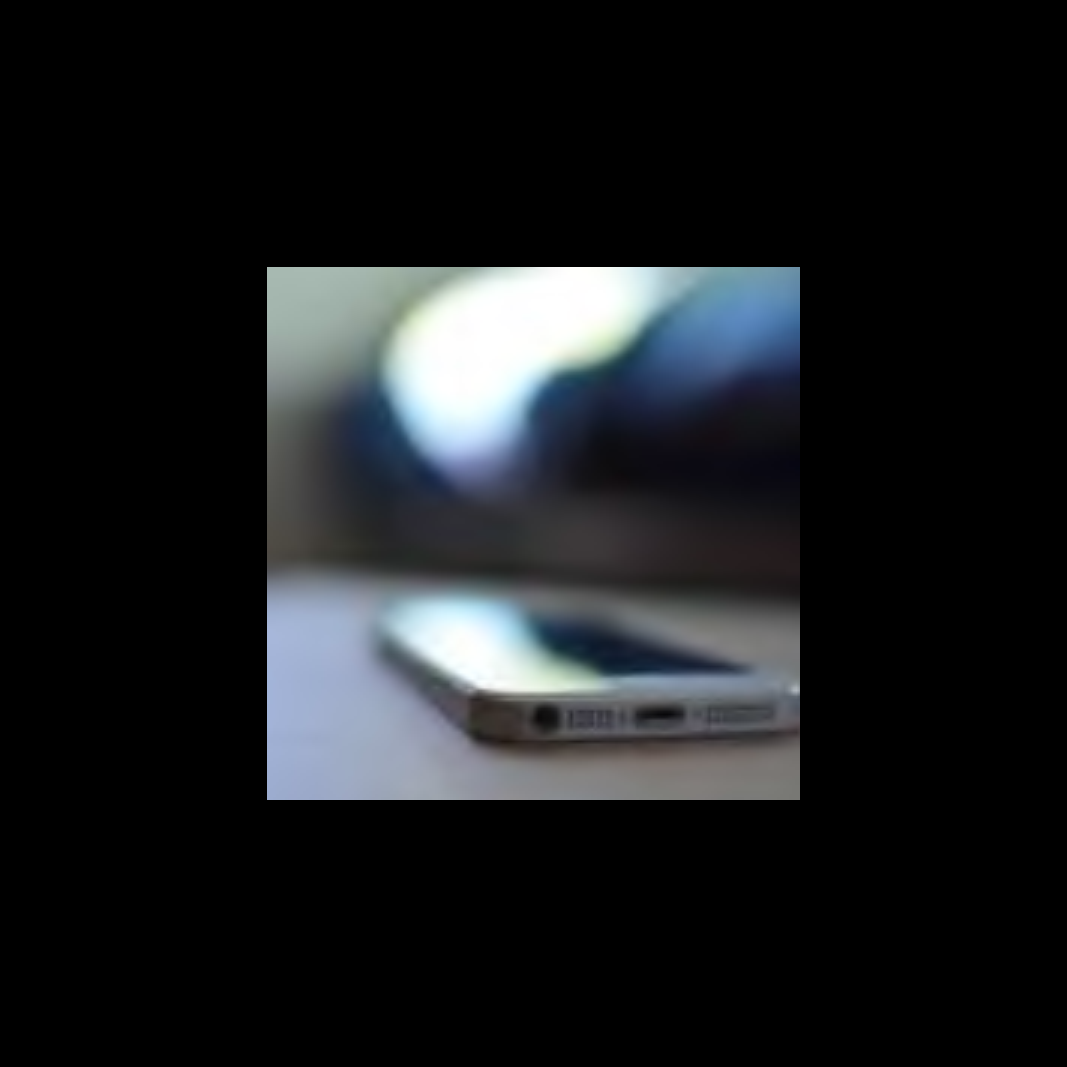
\includegraphics[width=8cm, height=8cm]{phone-geo-modified.png}
	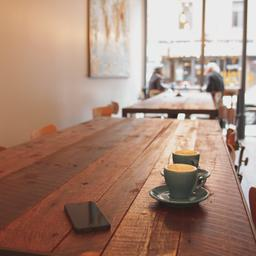
\includegraphics[width=8cm, height=8cm]{coffee-unmodified.jpg}
\end{figure}
\begin{figure}
	\caption{Po uruchomieniem algorytmu (od lewej): obraz 1 (256x256, 300dpi), obraz 2 (256x256, 300dpi)}
	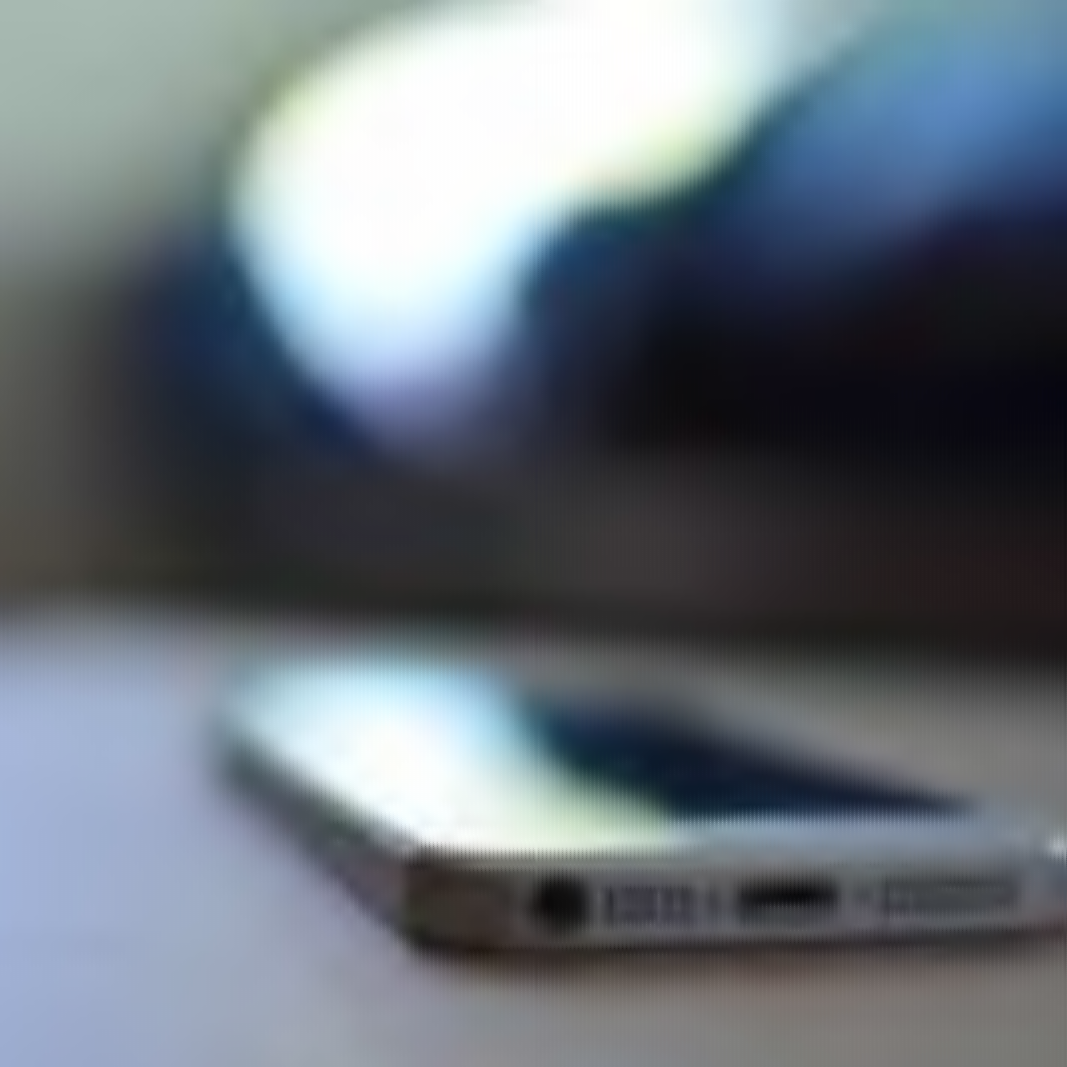
\includegraphics[width=8cm, height=8cm]{phone-rastar-unification.png}
	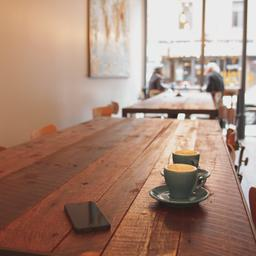
\includegraphics[width=8cm, height=8cm]{coffee-unmodified.jpg}
\end{figure}
\newpage
\subsection*{Kod źródłowy algorytmu}
\begin{python}
def rasterColor(self):
	print('rastar color unification start')
	self.firstDecoder.setColor()
	self._scaleUpColor(self.firstDecoder, 'Resources/rcUnification_1.png')
	print('first image done')
	self.secondDecoder.setColor()
	self._scaleUpColor(self.secondDecoder, 'Resources/rcUnification_2.png')
	print('second image done')
	print('rastar color unification done')

def _scaleUpColor(self, decoder, outputPath):
	width, height = decoder.width, decoder.height
	scaleFactoryW = float(self.maxWidth) / width
	scaleFactoryH = float(self.maxHeight) / height
	if width < self.maxWidth or height < self.maxHeight:
		pixelsBuffer = decoder.getPixels24Bits()
		result = numpy.full((self.maxHeight, self.maxWidth, 3), 1, numpy.uint8)
		# Fill values
		for h in range(height):
			for w in range(width):
				if w%2 == 0:
					result[int(scaleFactoryH * h), int(round(scaleFactoryW * w)) + 1] = pixelsBuffer[h, w]
				if w%2 == 1:
					result[int(round(scaleFactoryH * h)) + 1, int(scaleFactoryW * w)] = pixelsBuffer[h, w]
			# Interpolate
			self._interpolateColor(result)
			img = Image.fromarray(result, mode='RGB')
			img.save(outputPath)

def _interpolateColor(self, result):
	for h in range(self.maxHeight):
		for w in range(self.maxWidth):
			r, g, b = 0, 0, 0
			n = 0
			if (result[h, w][0] == 1) & (result[h, w][1] == 1) & (result[h, w][2] == 1):
				for hOff in range(-1, 2):
					for wOff in range(-1, 2):
						hSafe = h if ((h + hOff) > (self.maxHeight - 2)) | ((h + hOff) < 0) else (h + hOff)
						wSafe = w if ((w + wOff) > (self.maxWidth - 2)) | ((w + wOff) < 0) else (w + wOff)
						if (result[hSafe, wSafe][0] > 1) | (result[hSafe, wSafe][1] > 1) | (result[hSafe, wSafe][2] > 1):
							r += result[hSafe, wSafe][0]
							g += result[hSafe, wSafe][1]
							b += result[hSafe, wSafe][2]
							n += 1
				result[h, w] = (r/n, g/n, b/n)
\end{python}

\chapter{Operacje sumowania arytmetycznego obrazów szarych}
Obraz jest macierzą wartości co pozwala nam wykonywać na nich operacje arytmetyczne tak samo jak na zwykłych macierzach. 
Operacje takie jak: 
\renewcommand{\labelitemi}{$*$}
\begin{itemize}
	\item dodawanie,
	\item odejmowanie,
	\item mnożenie (wyjątkowo wykonywane inaczej niż w przypadku dwóch macierzy),
	\item dzielenie
\end{itemize}
obrazów może odbywać się w różnych kombinacjach rodzajów wartości: 
\renewcommand{\labelitemi}{$*$}
\begin{itemize}
	\item obraz z obrazem
	\item obraz ze stałą
\end{itemize}
Operacje te odbywają się na poziomie komórek macierz i są też nazywane \textbf{operatorami punktowymi}. Co oznacza, że przy przetwarzaniu dwóch obrazów liczą się tylko wartości znajdujące się na tej samej pozycji wysokości i szerokości w obrazie $P_1(i,j)$ i $P_2(i,j)$. 
\\
Po przeprowadzeniu niektórych operacji algebraicznych należy przeprowadzić normalizację w celu zmiany zakresu wartości \textit{(min, max)} na \textit{(newMin, newMax)}. 
Do przeprowadzenia normalizacji w poniższych przykładach będziemy używać wzoru: 
\[f_{norm}=Z_{rep}[(f-f_{min})/(f_{max}-f_{min})]\]
Gdzie $Z_{rep}$ oznacza maksymalną wartość dla naszej struktury piksela. Dla obrazów szarych może przybrać wartość \textit{\#FF} (system szesnastkowy) lub dla wersji kolorowej \textit{\#FFFFFF}. 
W celu uniknięcia powtórzeń w kodzie źródłowym wydzieliłem funkcję normalizacji, która dla obrazów szarych prezentuje się następująco: 
\inputpython{../Source/Commons.py}{8}{15}

\section{Sumowanie określonej stałej z obrazem}
\subsection*{Algorytm}
\subsubsection*{Opis}
W operacji sumowania obrazów szarych ze stałą ważne jest doprowadzenie do stanu w którym będziemy mogli dodać wartość 
nie martwiąc się o przepełnienie zmiennej co mogłoby spowodować zniekształcenie obrazu. \\
Aby tego uniknąć przeskalujemy wszystkie wartości macierzy obrazu tak, aby suma stałej i największej wartości macierzy 
nie przekroczyła maksymalnej wartości dla zmiennej. 

\begin{figure}[H]
	\caption{Przed uruchomieniem algorytmu (lewy obraz), po dodaniu wartości 30 (środkowy obraz), po normalizacji (prawy obraz)}
	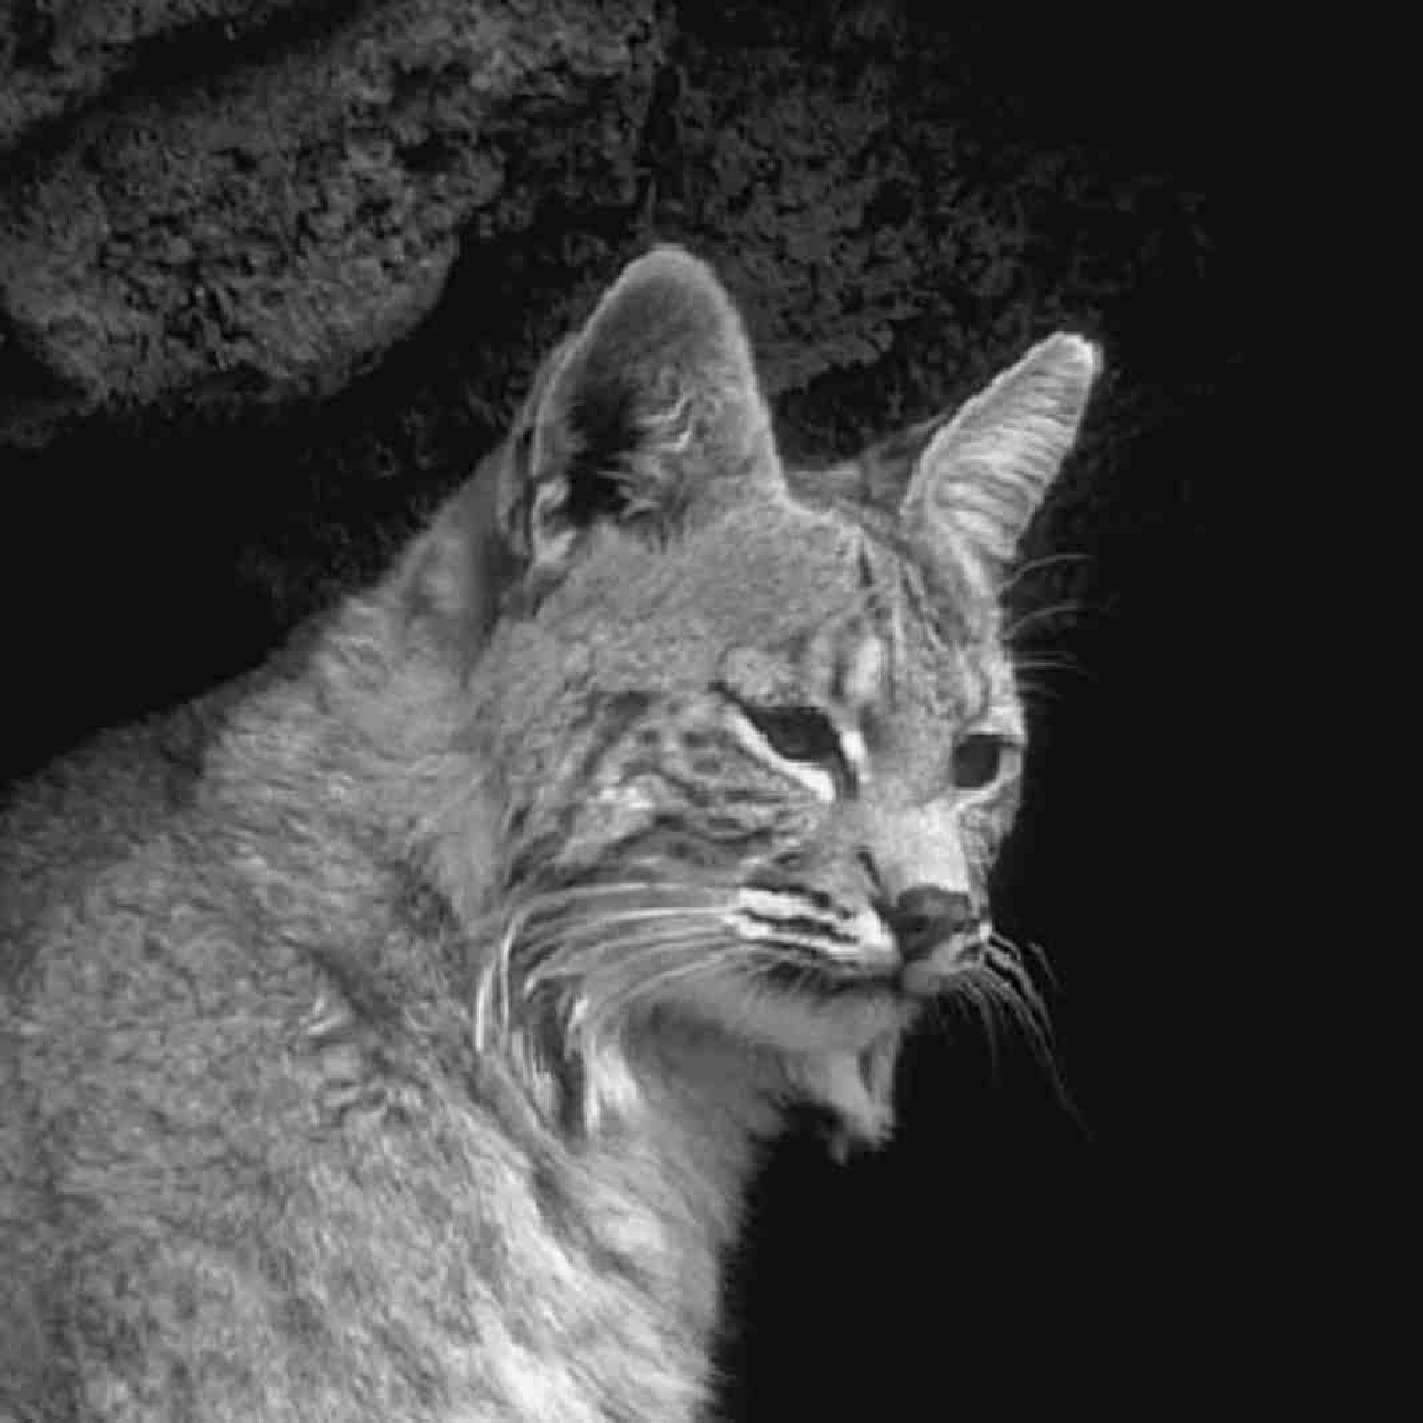
\includegraphics[width=5cm, height=5cm]{cat-unmodified.jpg}
	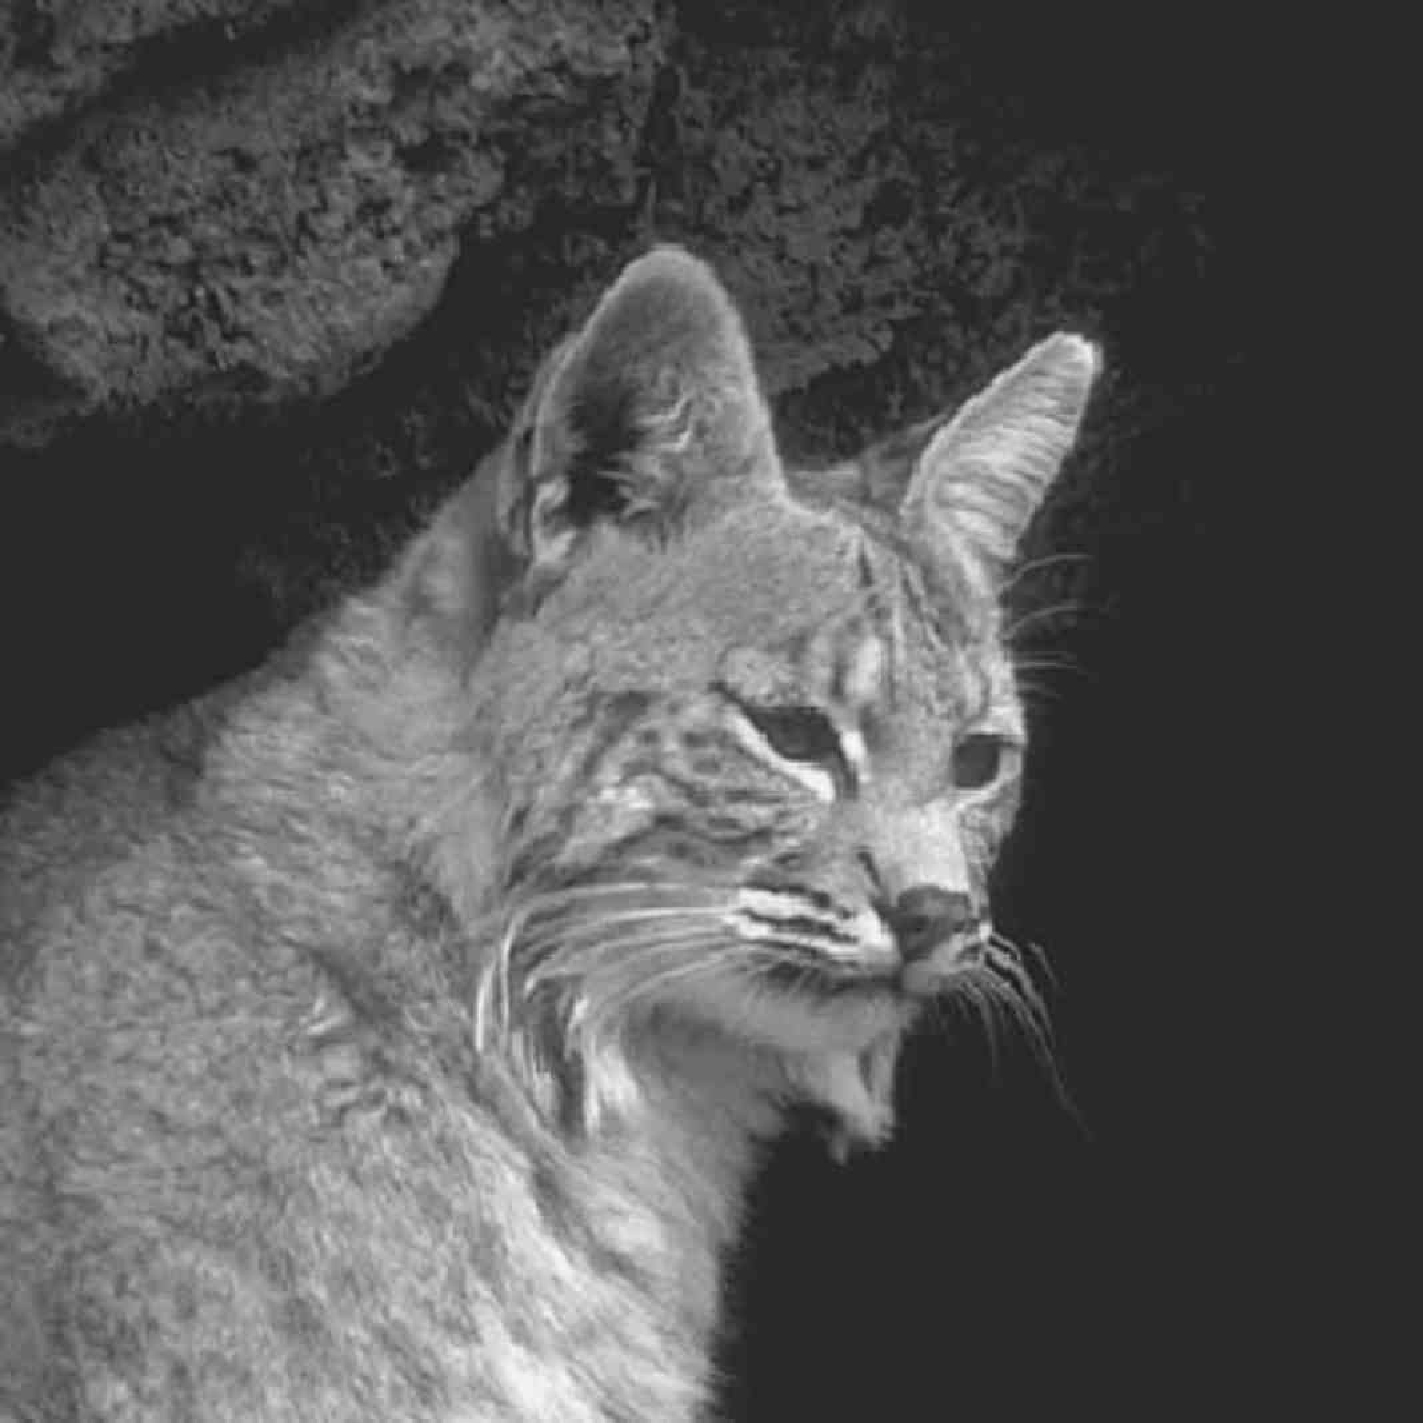
\includegraphics[width=5cm, height=5cm]{2/sum-gray-const-30.png}
	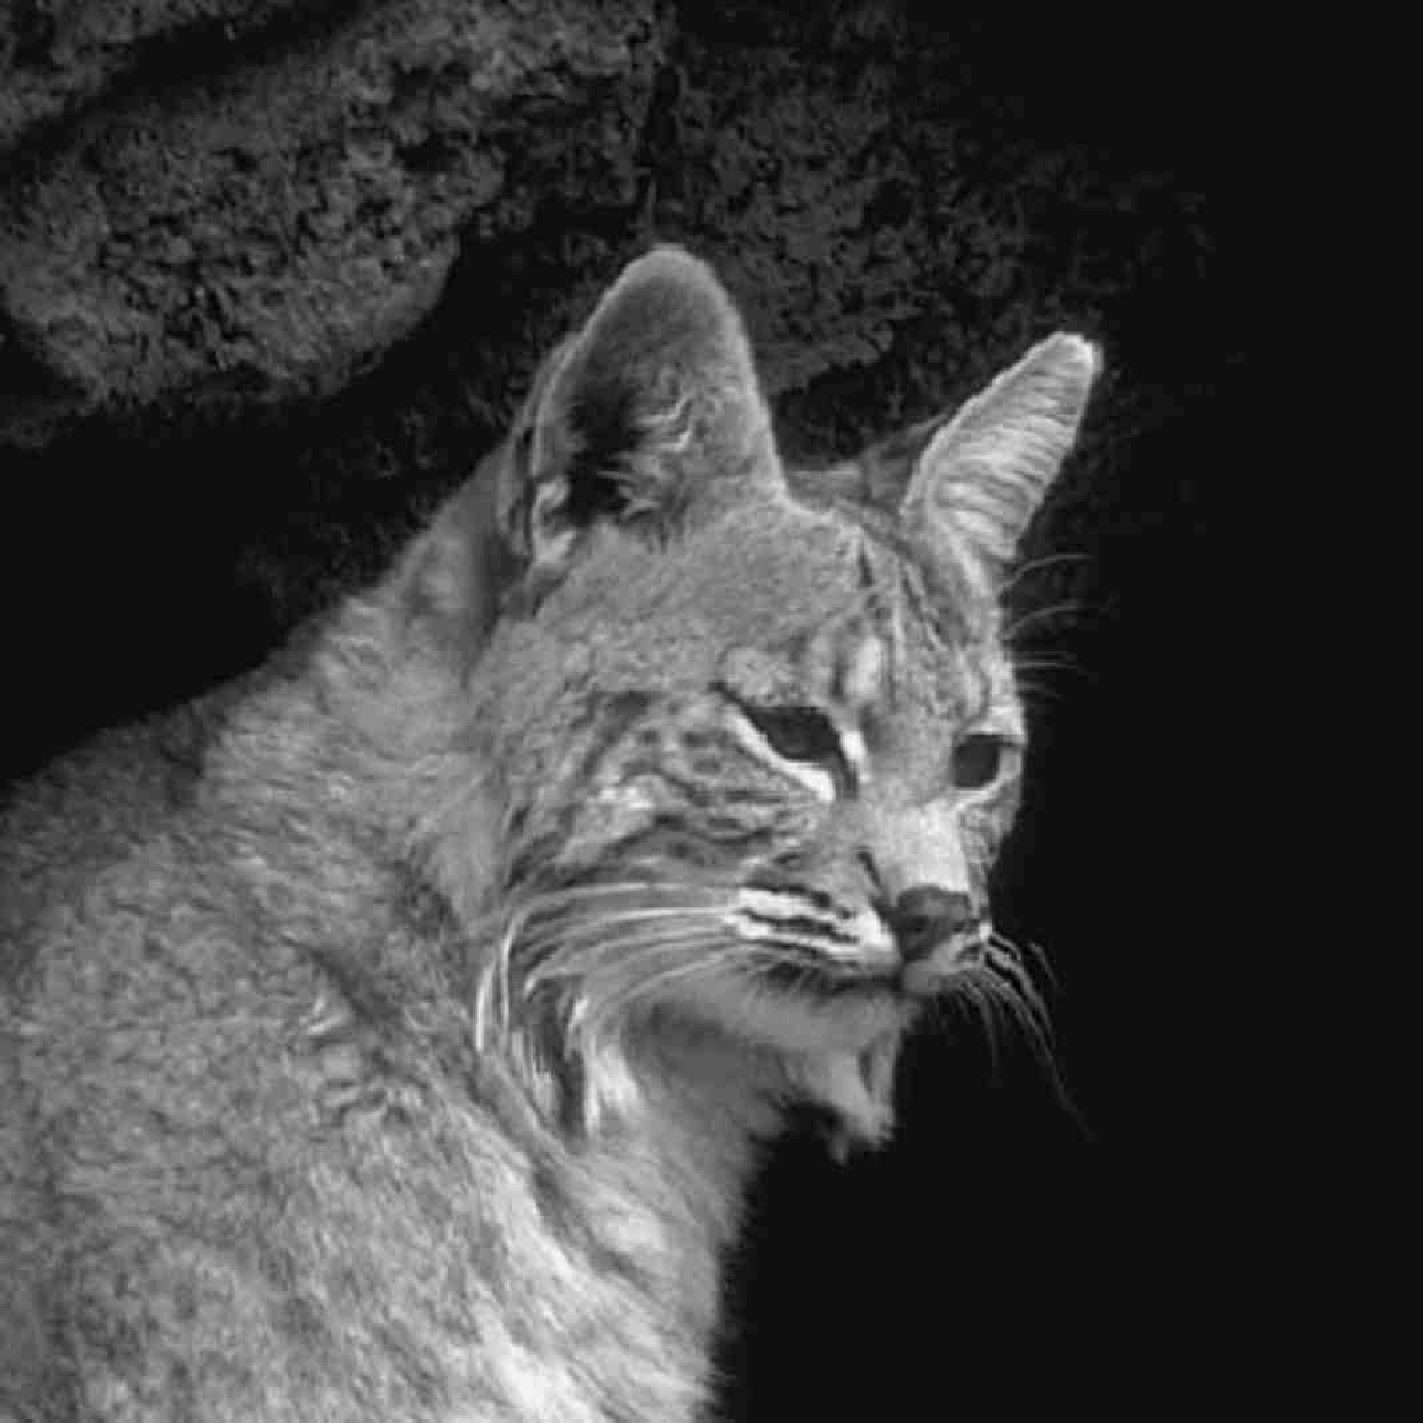
\includegraphics[width=5cm, height=5cm]{2/sum-gray-const-30-norm.png}
\end{figure}
\begin{figure}[H]
	\caption{Przed uruchomieniem algorytmu (lewy obraz), po dodaniu wartości 300 (środkowy obraz), po normalizacji (prawy obraz)}
	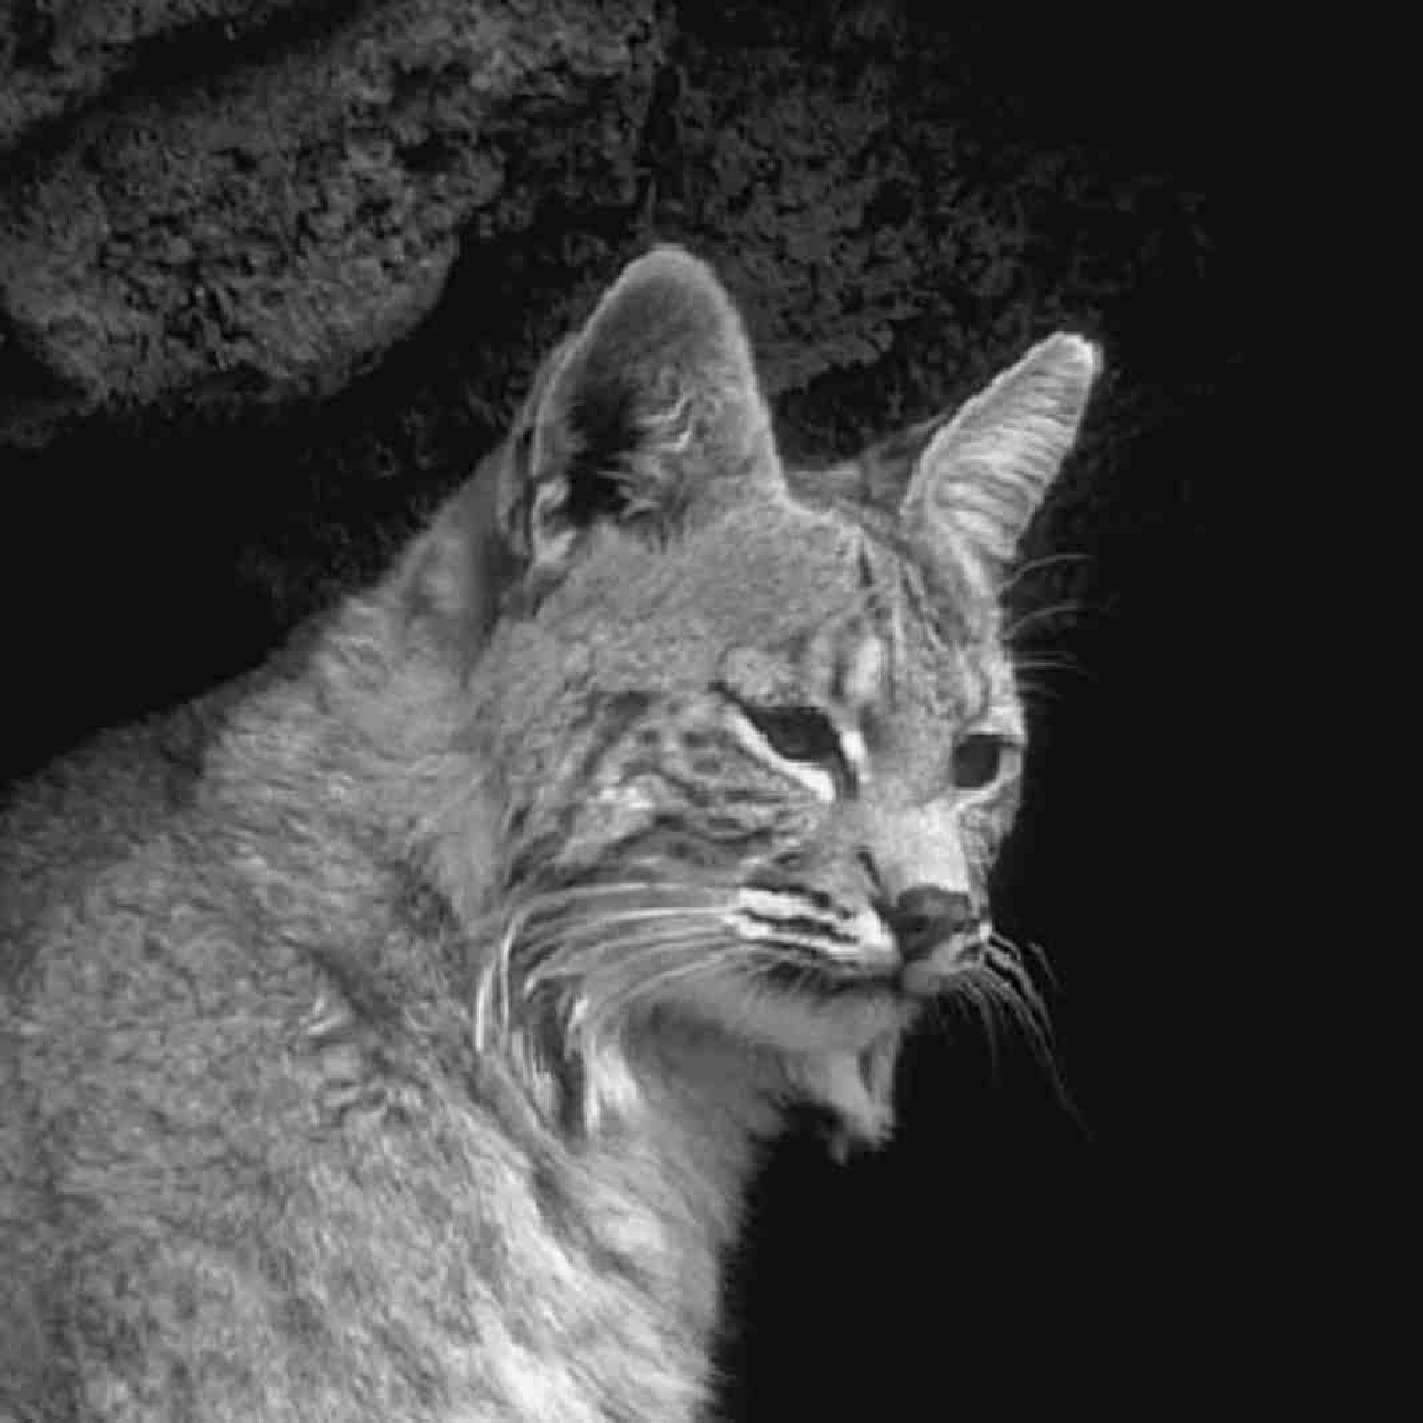
\includegraphics[width=5cm, height=5cm]{cat-unmodified.jpg}
	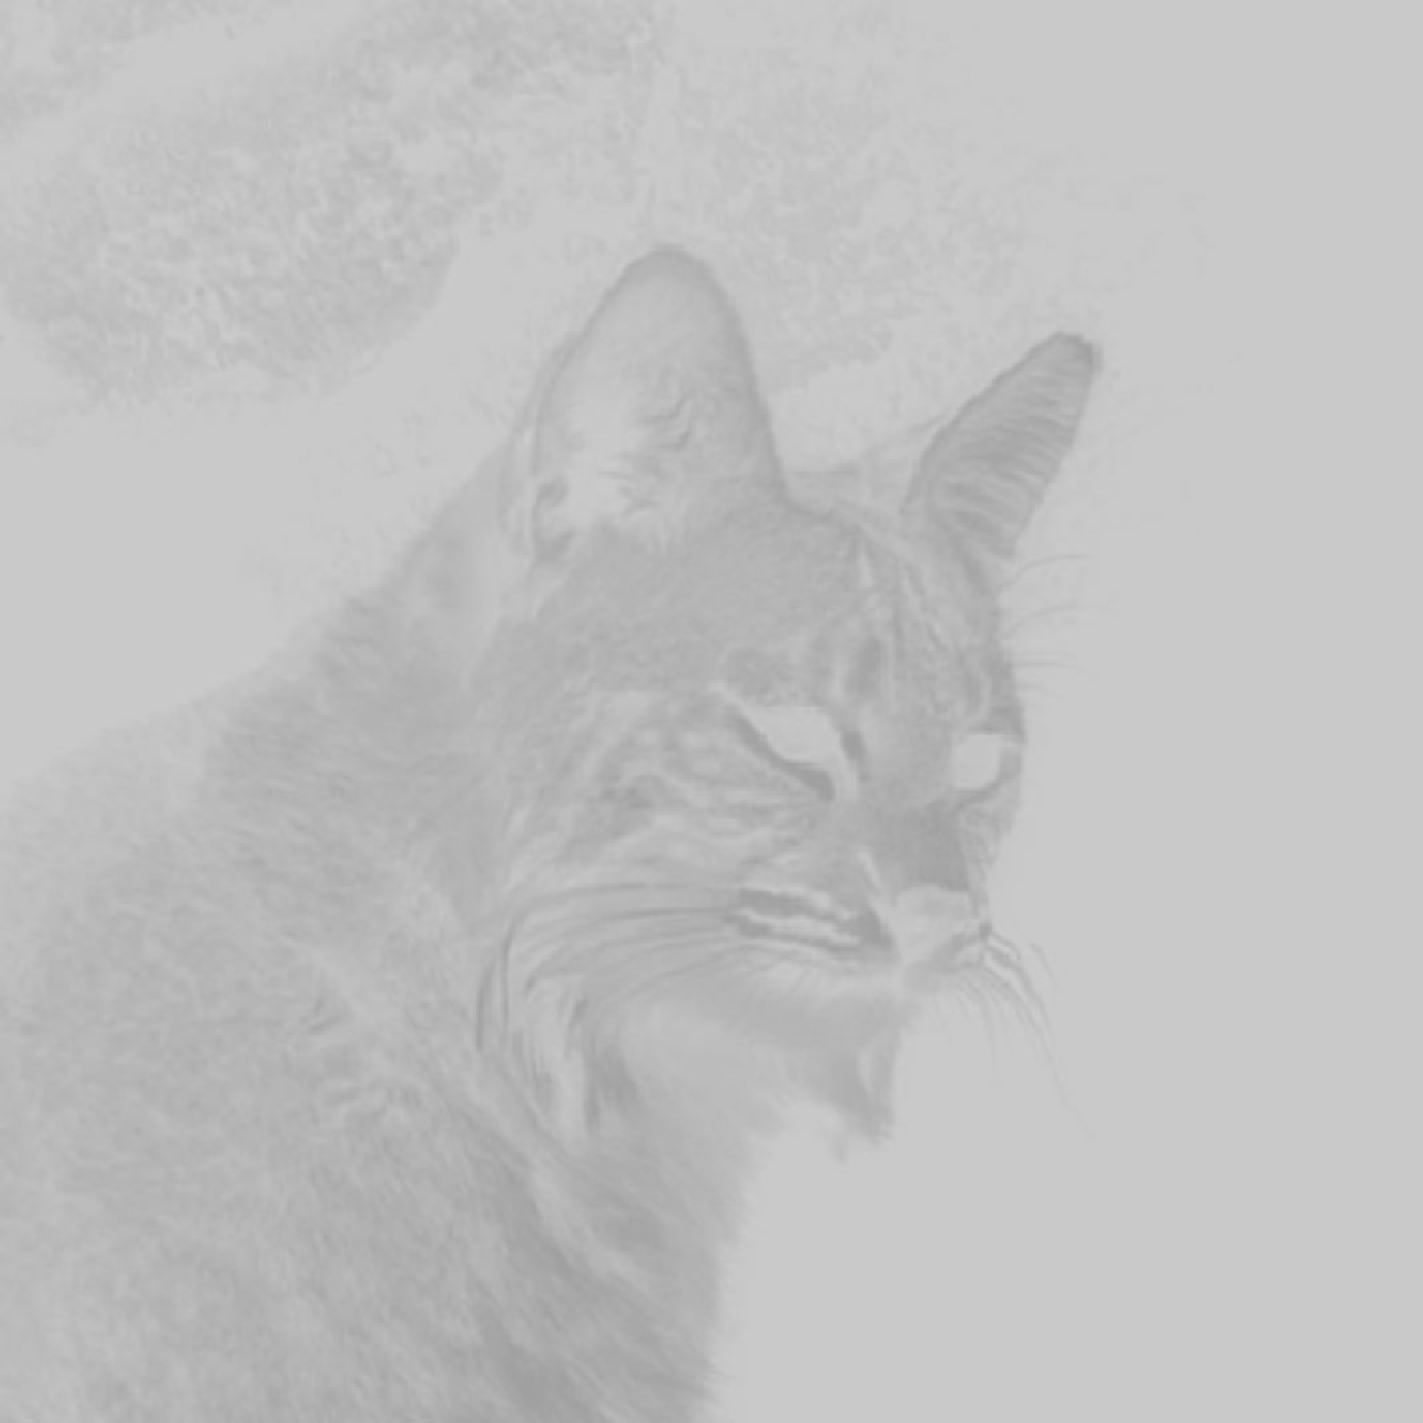
\includegraphics[width=5cm, height=5cm]{2/sum-gray-const-300.png}
	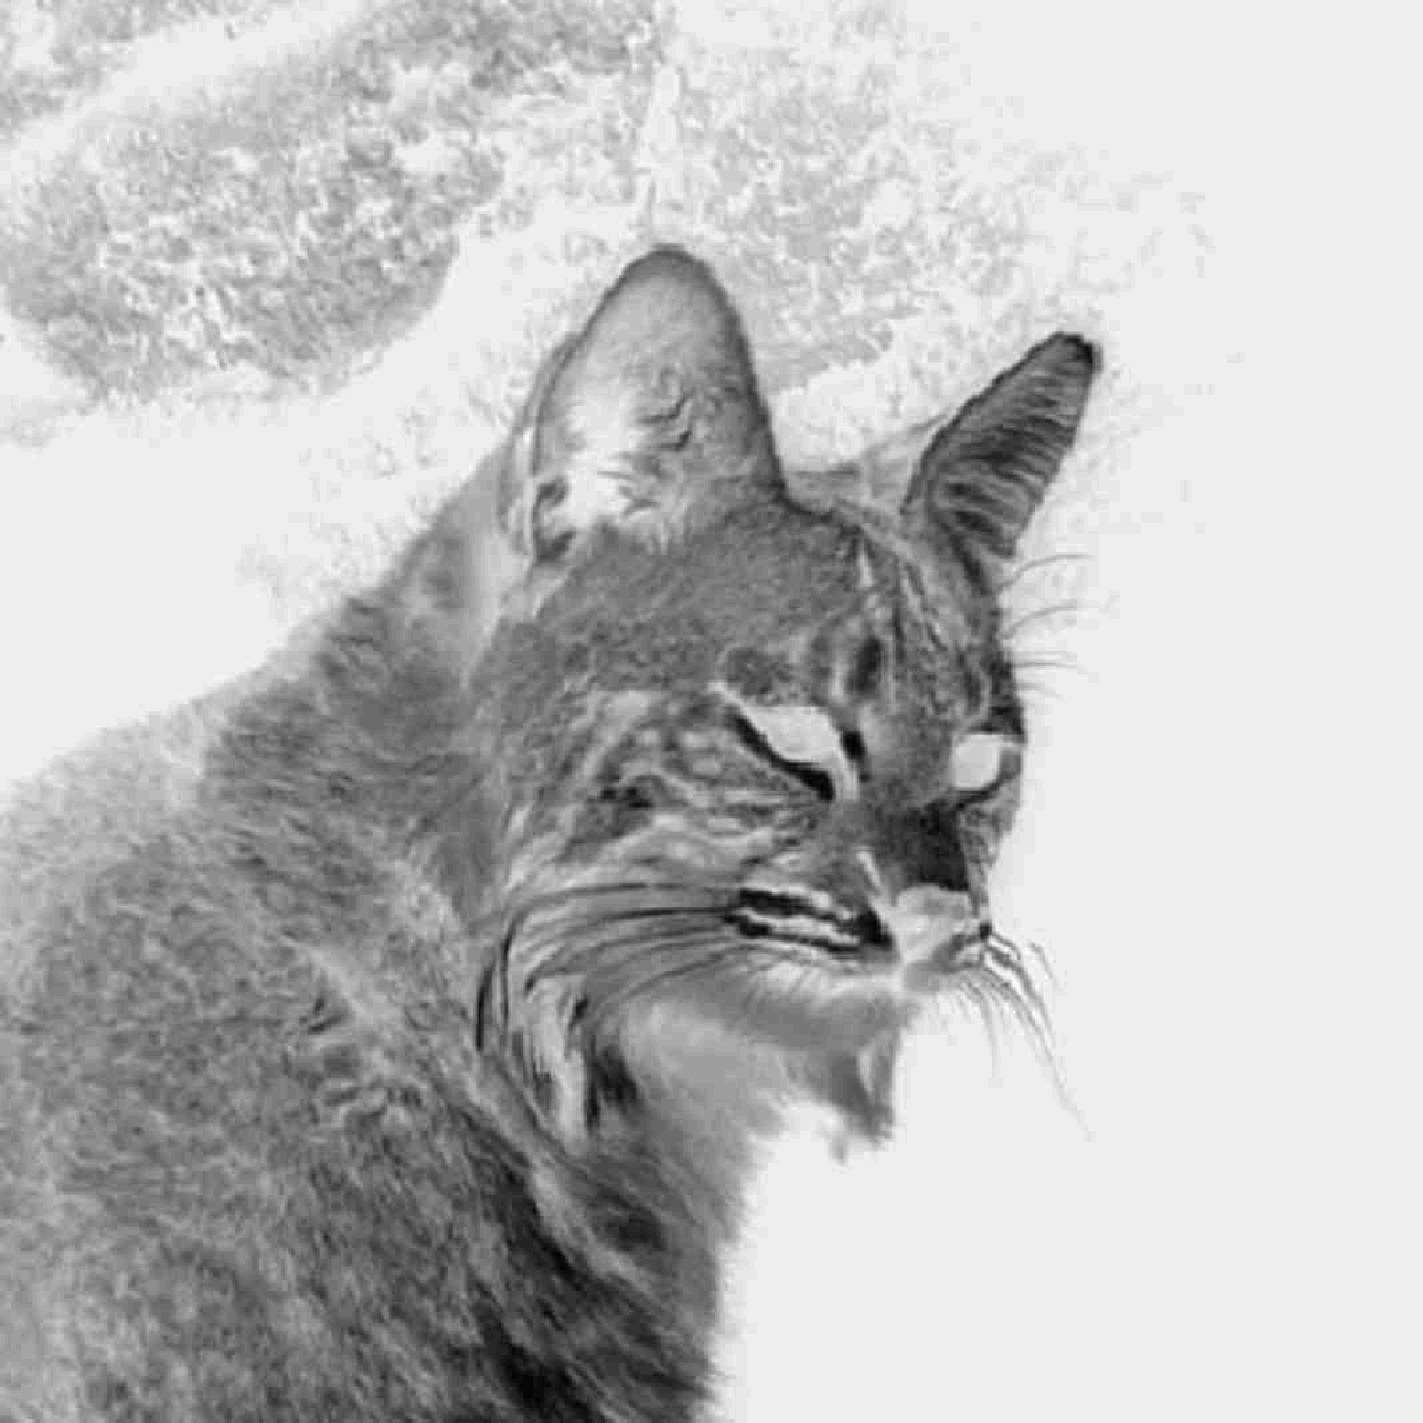
\includegraphics[width=5cm, height=5cm]{2/sum-gray-const-300-norm.png}
\end{figure}
\begin{figure}[H]
	\caption{Przed uruchomieniem algorytmu (lewy obraz), po dodaniu wartości 30 (środkowy obraz), po normalizacji (prawy obraz)}
	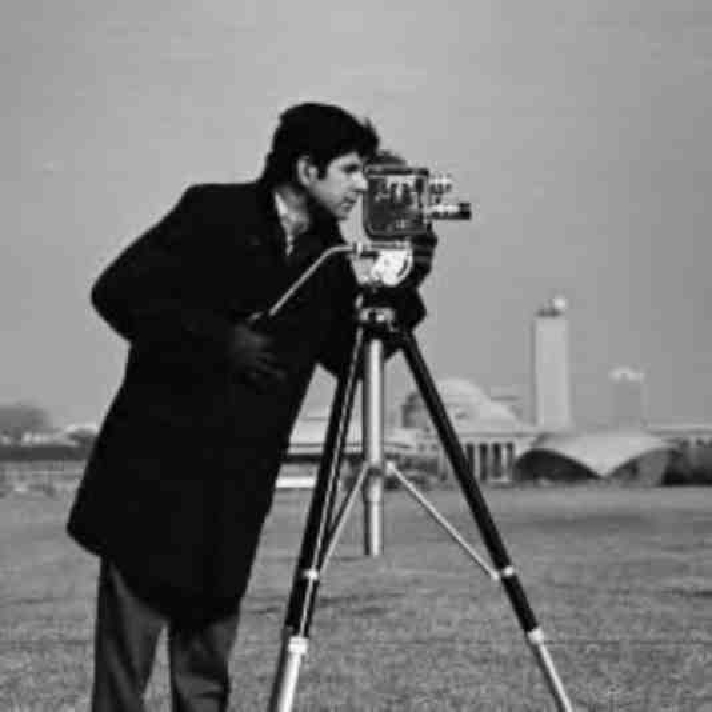
\includegraphics[width=5cm, height=5cm]{man-unmodified.jpg}
	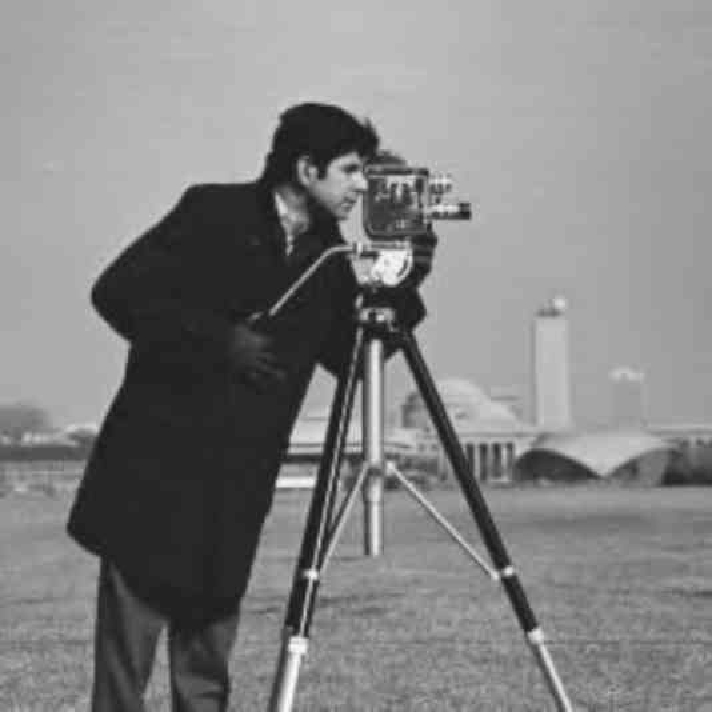
\includegraphics[width=5cm, height=5cm]{2/sum-gray-const-30-2.png}
	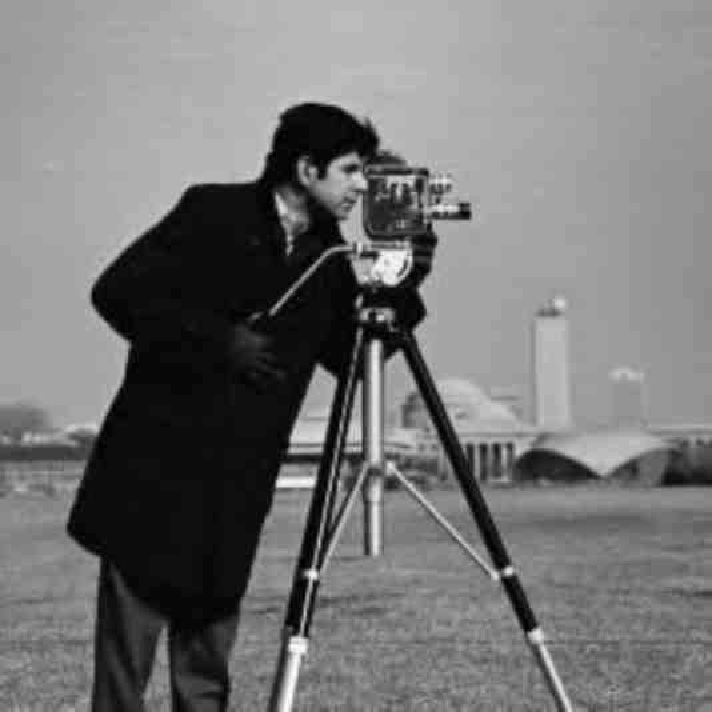
\includegraphics[width=5cm, height=5cm]{2/sum-gray-const-30-norm-2.png}
\end{figure}
\begin{figure}[H]
	\caption{Przed uruchomieniem algorytmu (lewy obraz), po dodaniu wartości 300 (środkowy obraz), po normalizacji (prawy obraz)}
	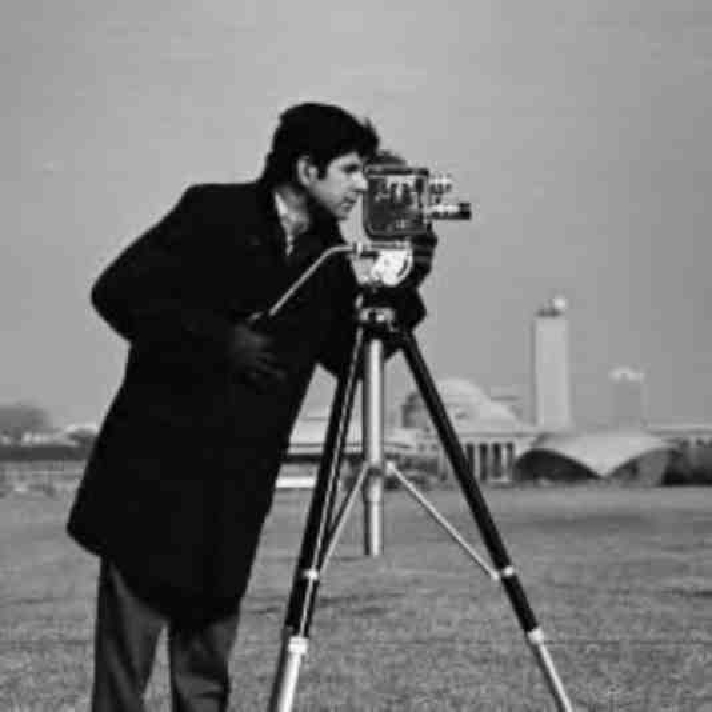
\includegraphics[width=5cm, height=5cm]{man-unmodified.jpg}
	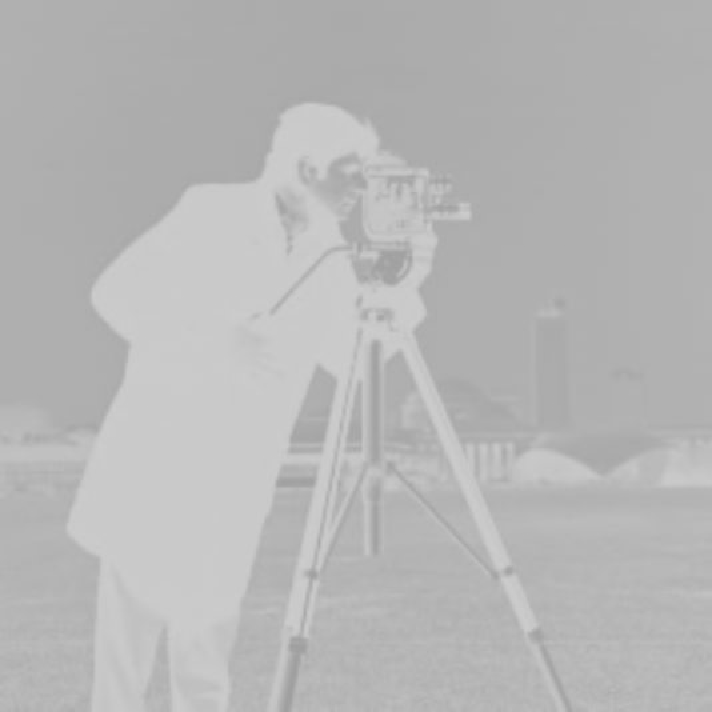
\includegraphics[width=5cm, height=5cm]{2/sum-gray-const-300-2.png}
	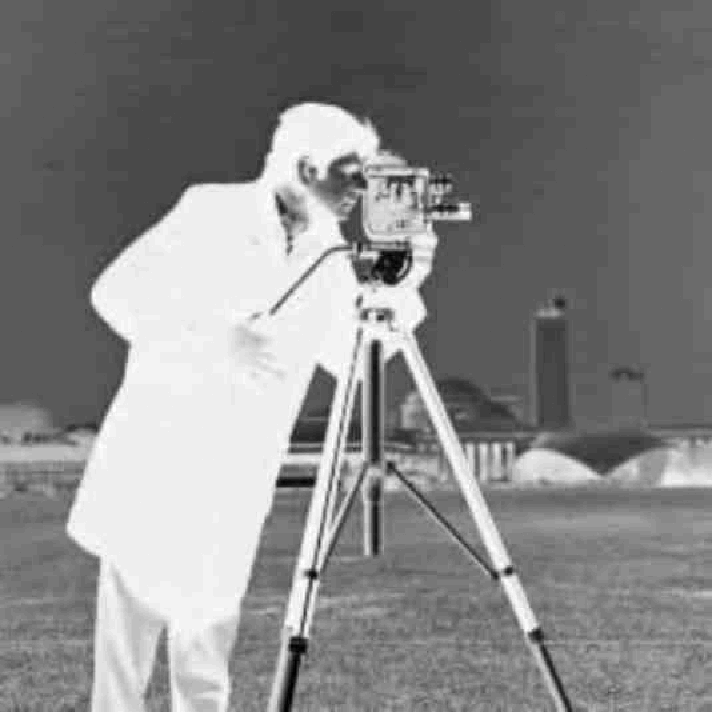
\includegraphics[width=5cm, height=5cm]{2/sum-gray-const-300-norm-2.png}
\end{figure}

\subsection*{Kod źródłowy programu}
\inputpython{../Source/ArithmeticSumGray.py}{18}{35}

\section{Sumowanie dwóch obrazów}
\subsection*{Algorytm}
\subsubsection*{Opis}
Dodanie dwóch obrazów jest analogiczne jak przy dodaniu stałej do obrazu, ale z tą różnicą, że maksymalnej wartości mogącej spowodować przepełnienie szukamy we wstępnym obrazie wynikowym sumy obu obrazów. 

\begin{figure}[H]
	\caption{Przed uruchomieniem algorytmu (obrazy na górze), po dodaniu obrazów (lewy, dolny obraz), po normalizacji (prawy, dolny obraz)}
	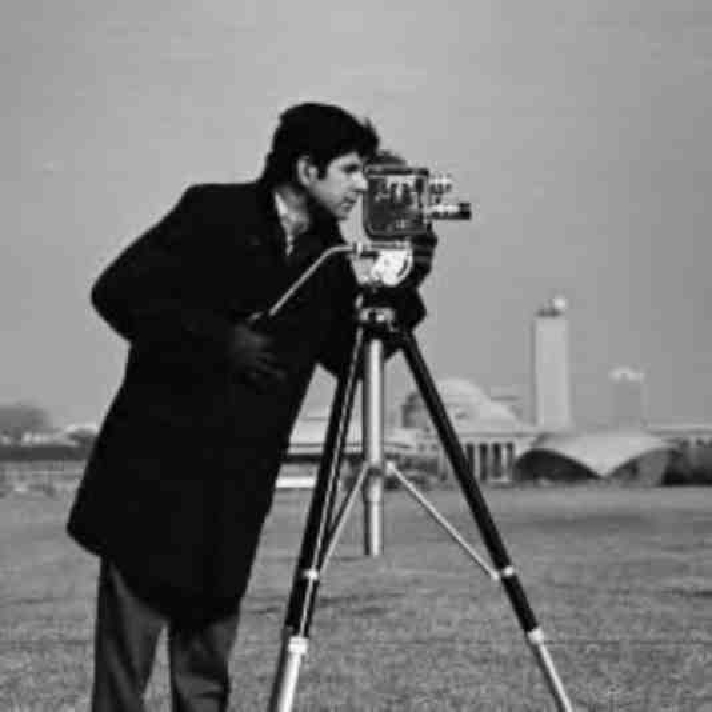
\includegraphics[width=7cm, height=7cm]{man-unmodified.jpg}
	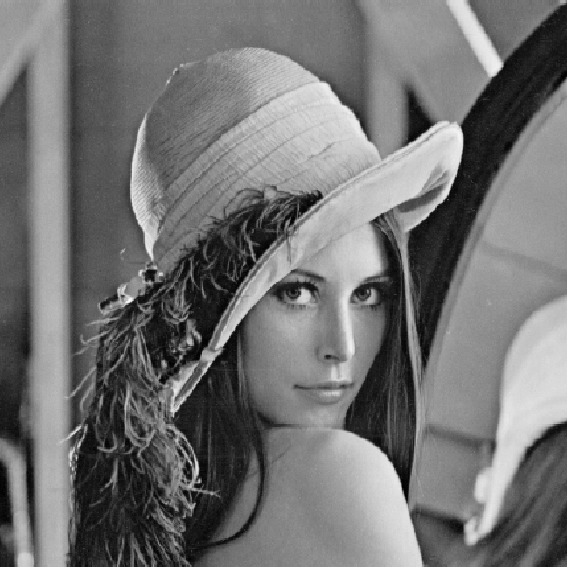
\includegraphics[width=7cm, height=7cm]{lena-unmodified.png}
	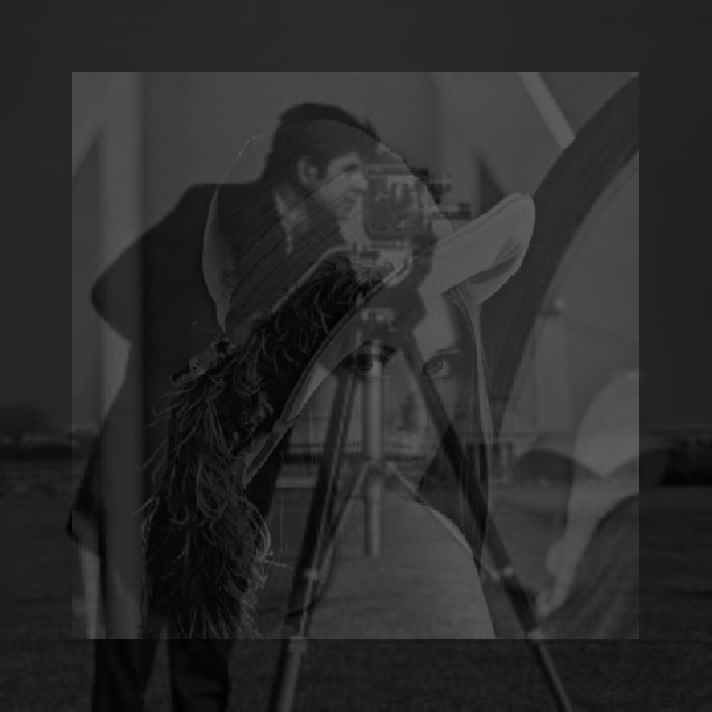
\includegraphics[width=7cm, height=7cm]{2/sum-gray-images.png}
	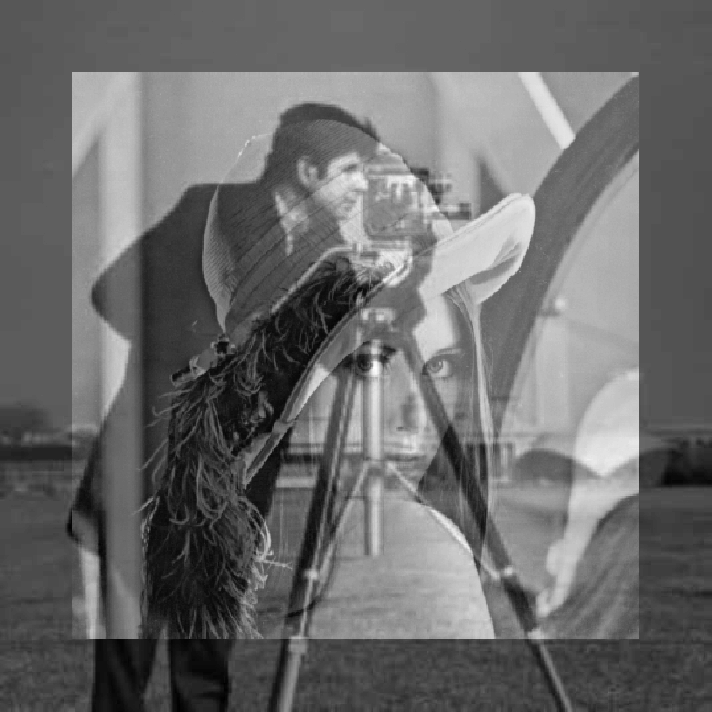
\includegraphics[width=7cm, height=7cm]{2/sum-gray-images-norm.png}
\end{figure}
\begin{figure}[H]
	\caption{Przed uruchomieniem algorytmu (obrazy na górze), po dodaniu obrazów (lewy, dolny obraz), po normalizacji (prawy, dolny obraz)}
	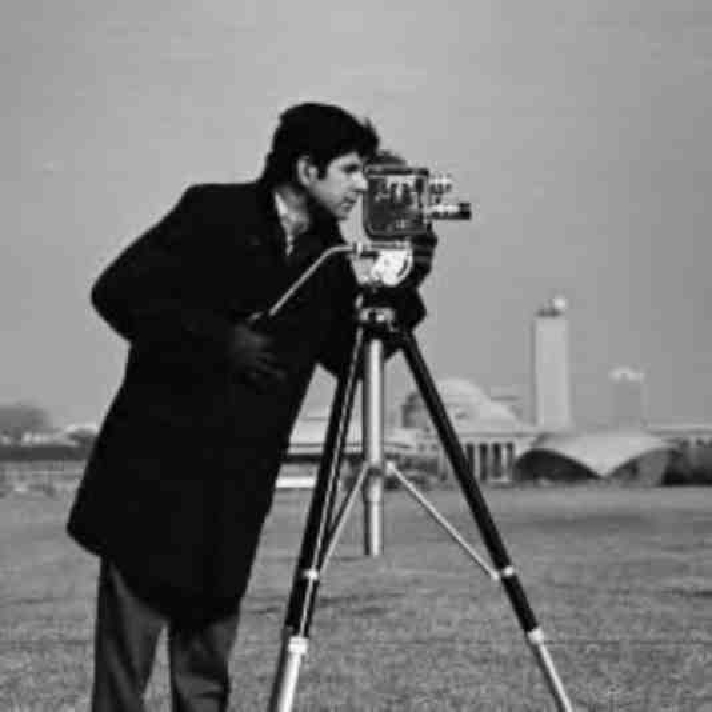
\includegraphics[width=7cm, height=7cm]{man-unmodified.jpg}
	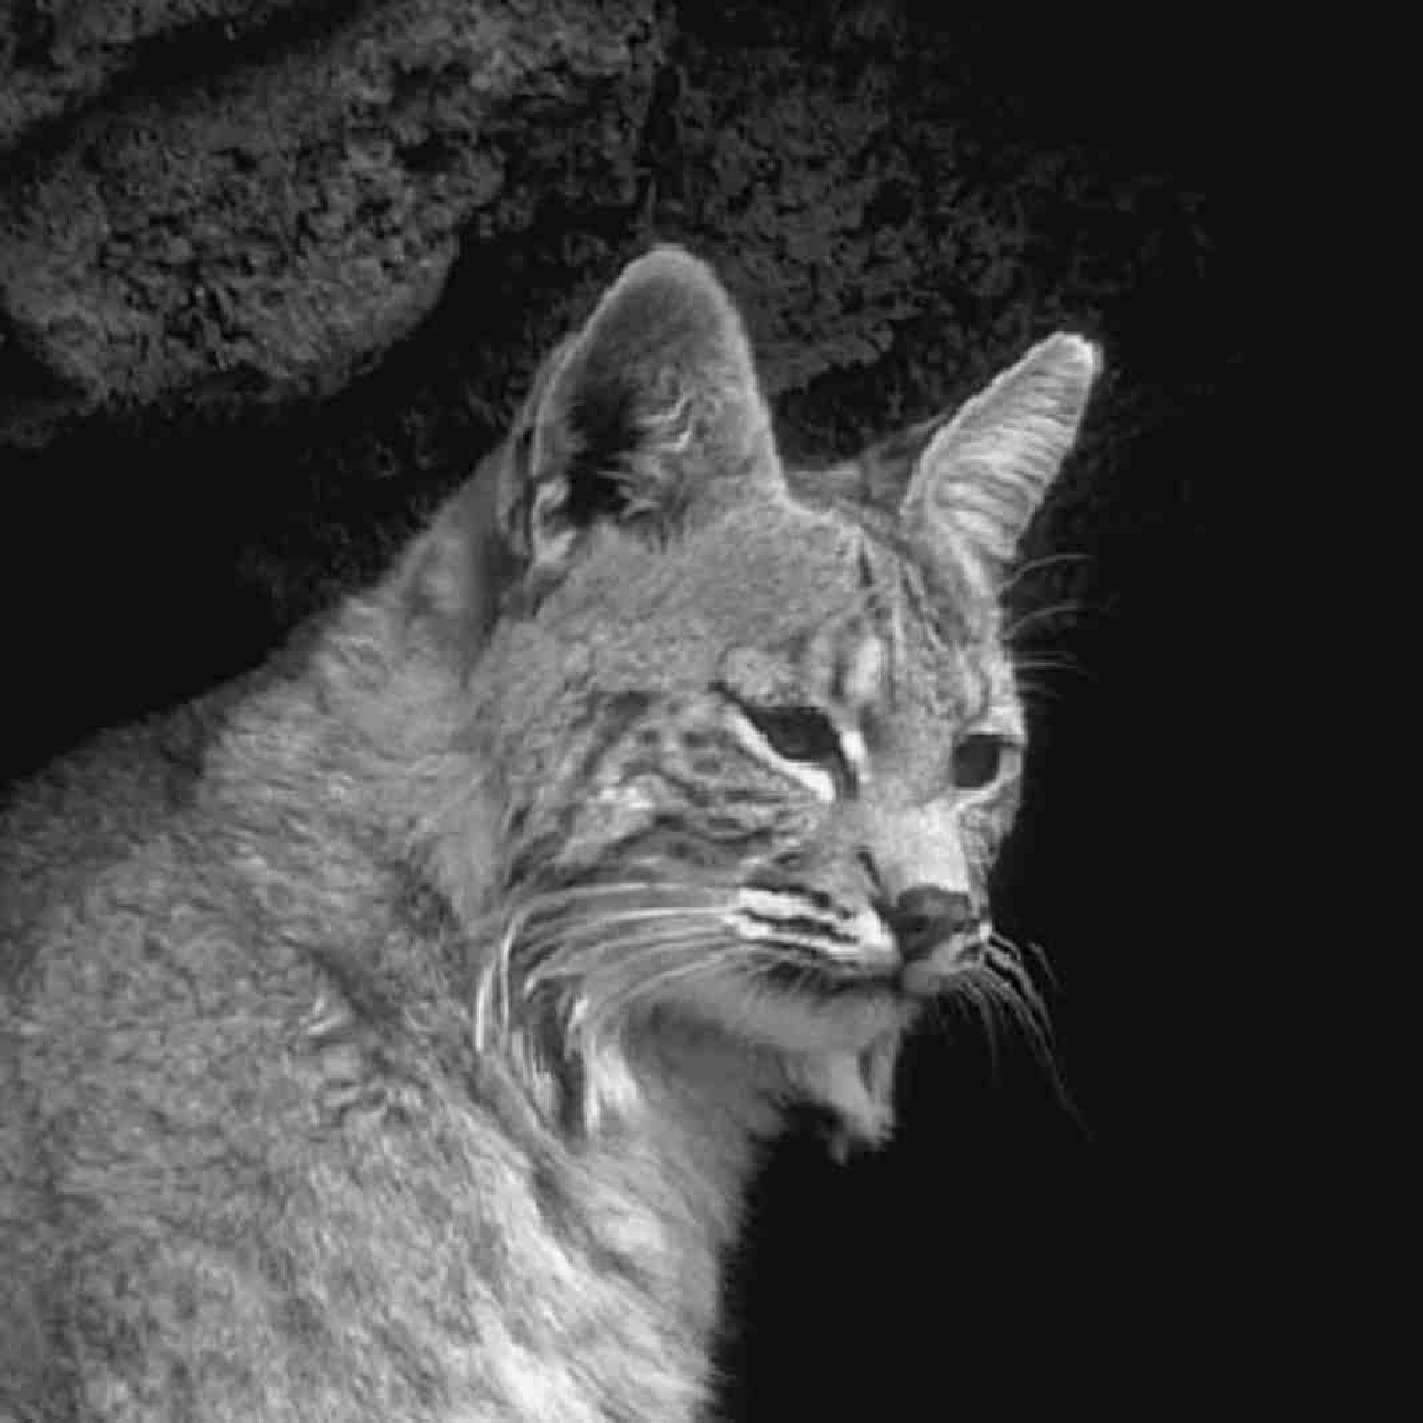
\includegraphics[width=7cm, height=7cm]{cat-unmodified.jpg}
	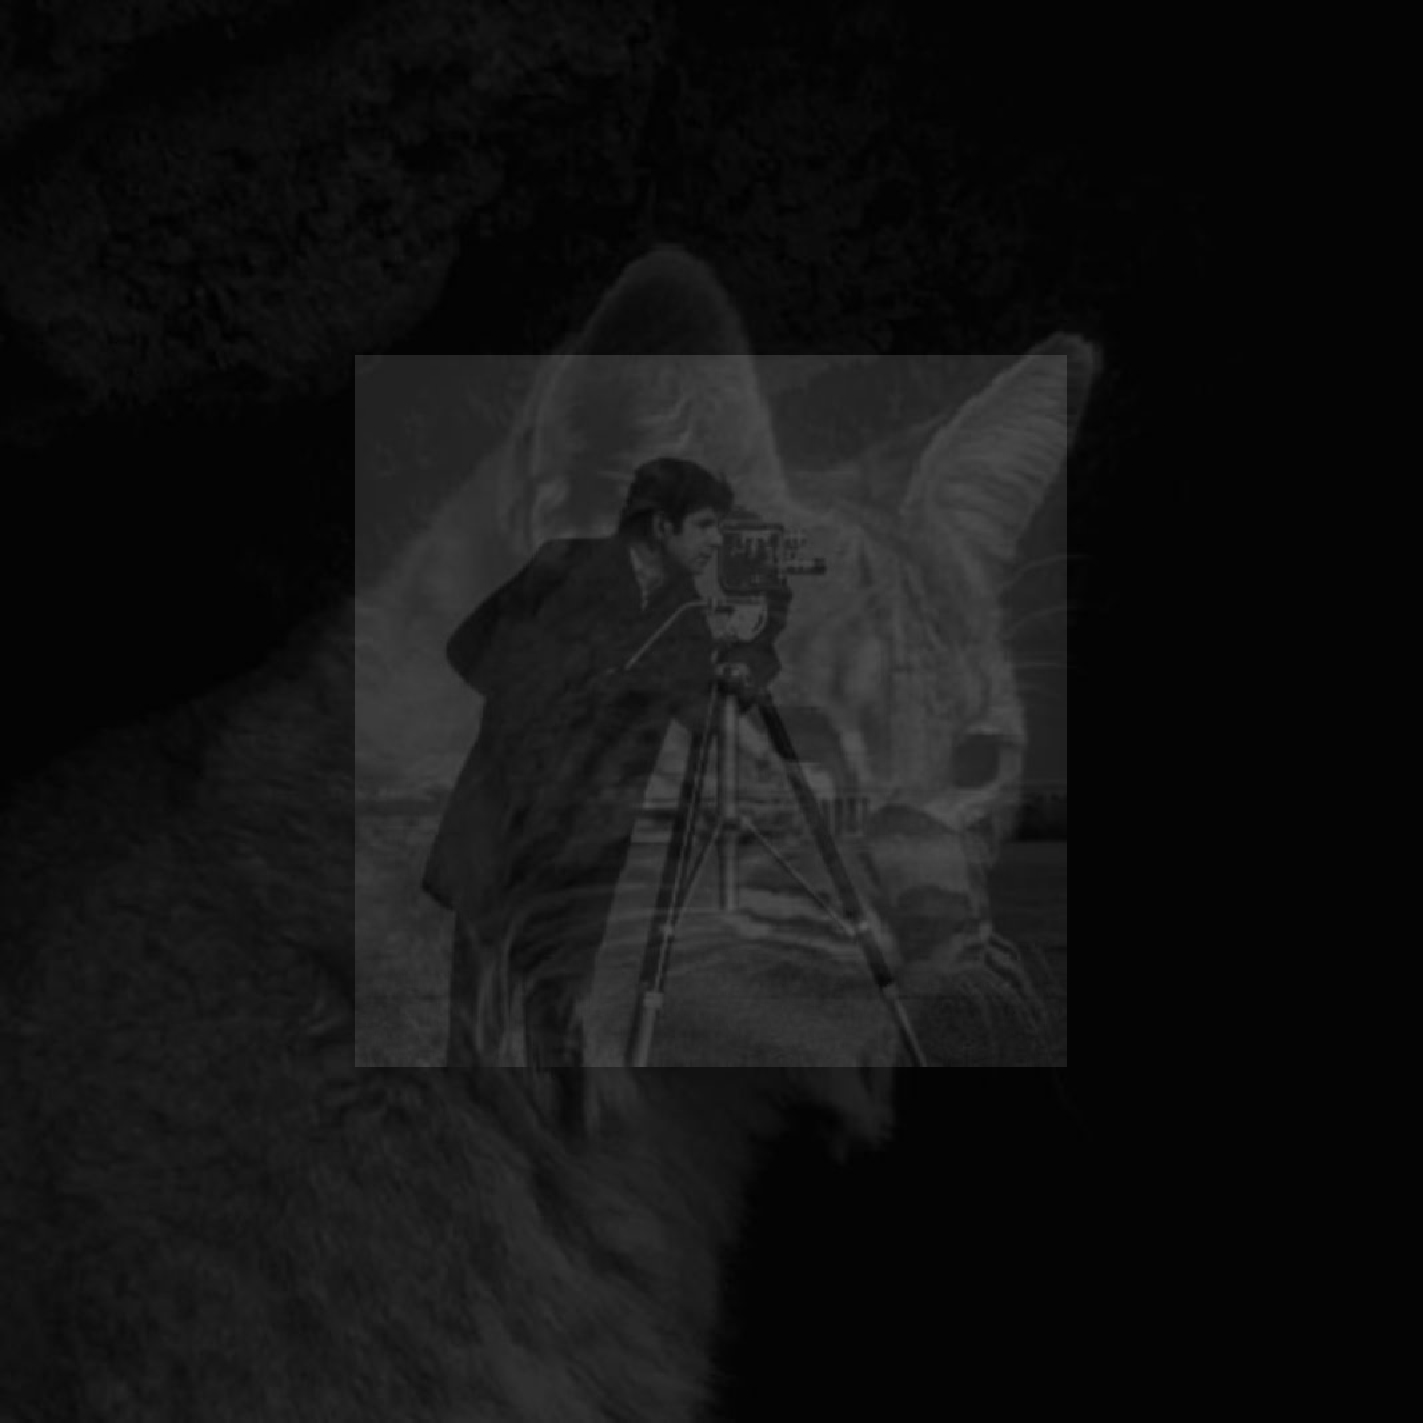
\includegraphics[width=7cm, height=7cm]{2/sum-gray-images-2.png}
	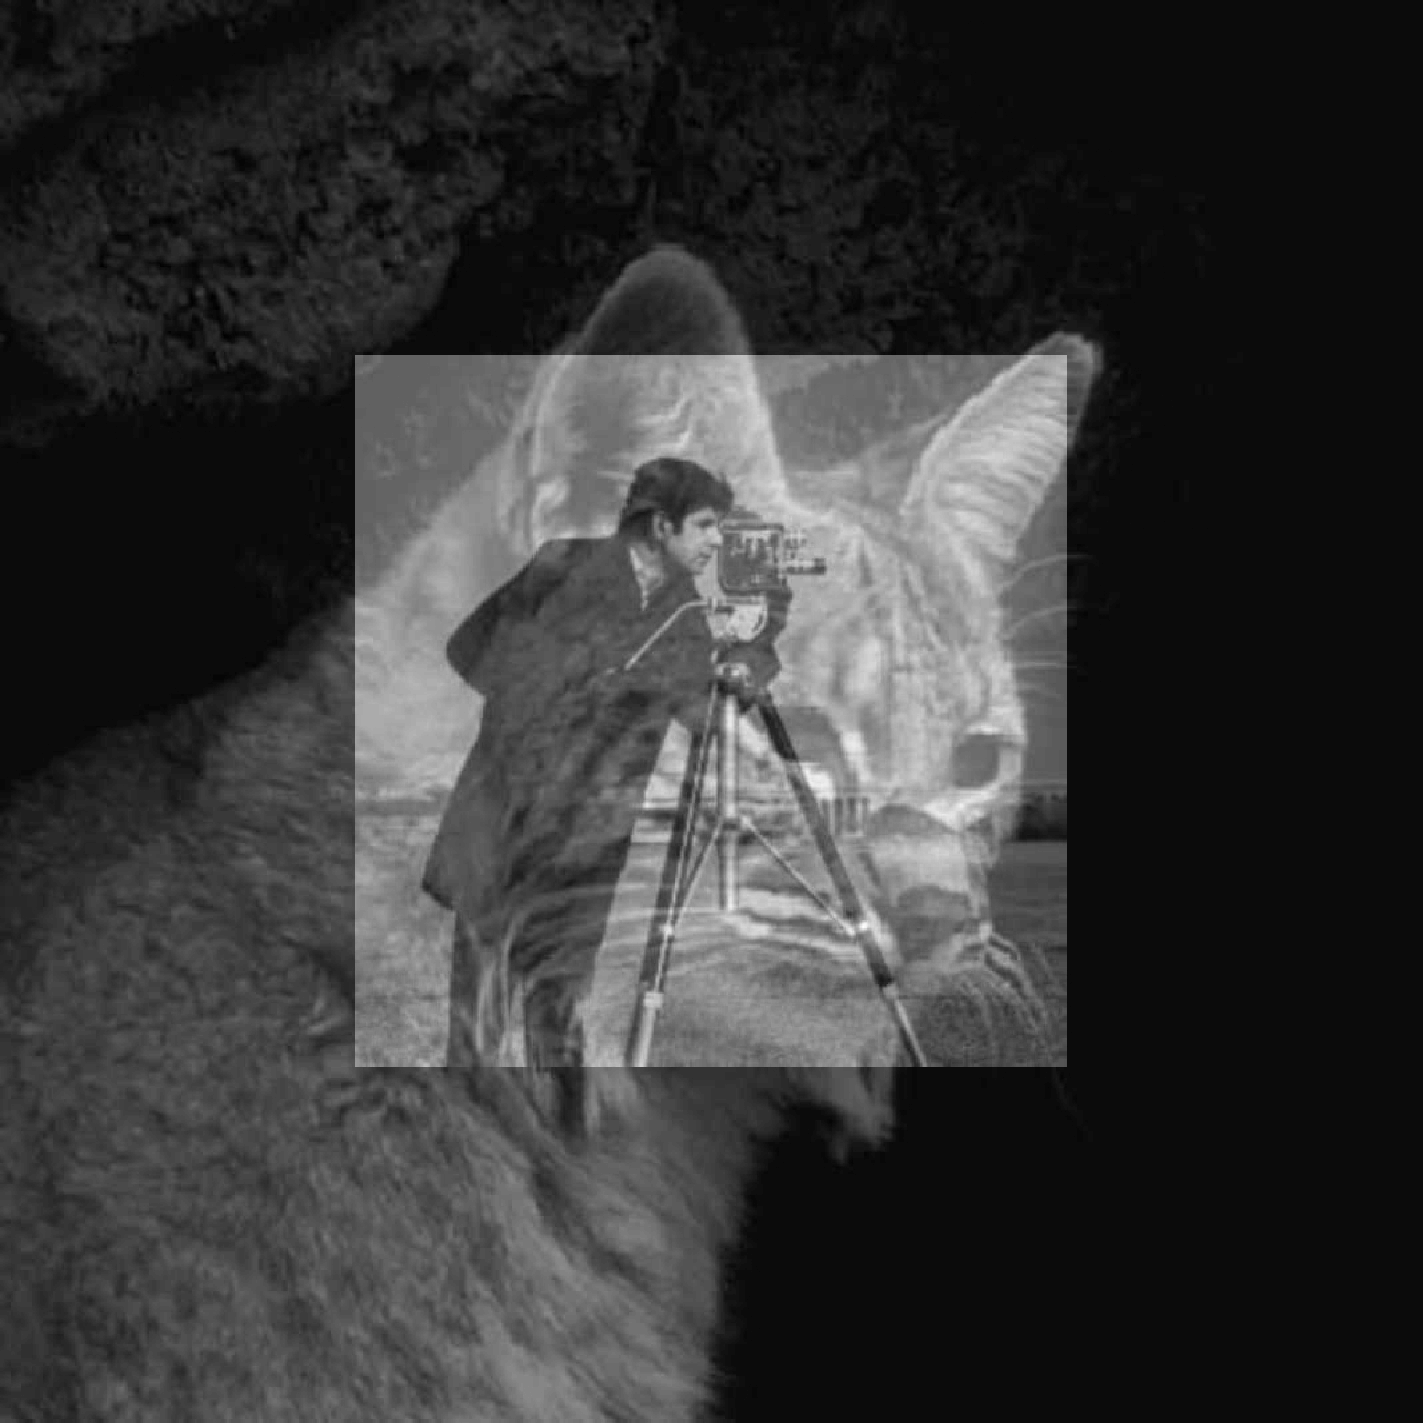
\includegraphics[width=7cm, height=7cm]{2/sum-gray-images-2-norm.png}
\end{figure}

\subsection*{Kod źródłowy programu}
\inputpython{../Source/ArithmeticSumGray.py}{38}{59}

\section{Mnożenie obrazu przez zadaną liczbę}
\subsection*{Algorytm}
\subsubsection*{Opis}
Mnożenie obrazu przychodzi w dwóch formach. Jednym z nich jest wykonanie tej operacji z użyciem stałej jako mnożnika. Na wykonanie tej czynności składa się mnożenie każdego z pikseli przez stałą, w ten sam sposób jak przy zwykłych macierzach: \\
$
\begin{bmatrix}
a_{11} & a_{12} & a_{13}\\
a_{21} & a_{22} & a_{23}\\
a_{31} & a_{32} & a_{33}
\end{bmatrix}
* X = 
\begin{bmatrix}
a_{11} * X & a_{12} * X & a_{13} * X\\
a_{21} * X & a_{22} * X & a_{23} * X\\
a_{31} * X & a_{32} * X & a_{33} * X
\end{bmatrix}
$
\\\\
Mnożeniem obrazów szarych można nazwać też ich \textit{skalowaniem} i dla wartości $\{x: 0 < x < 1\}$ przyciemnij obrazy, a dla wartości $\{x: 1 < x\}$ rozjaśnij go. 
Jednym z zagrożeń przy tej operacji jest przepełnienie, które objawia się czarnymi plamami (Rysunek 3.7). Aby go uniknąć dla wartości powyżej  $Z_{rep}$ (tzn. maksymalna wielkość zakresu reprezentacji tonalnej obrazu) program przytnie wartości do $Z_{rep}$ co będzie skutkowało coraz jaśniejszymi obrazami, a uniemożliwi czarne plamy. 

\begin{figure}[H]
	\caption{Przykład przekroczenia maksymalnej wartości}
	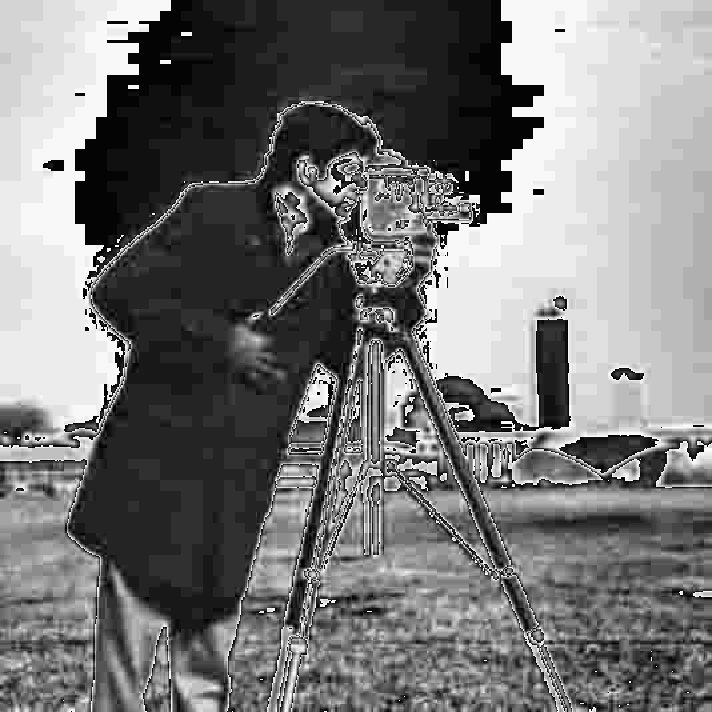
\includegraphics[width=17cm, height=17cm]{2/multiply-gray-const-error.png}
\end{figure}

\begin{figure}[H]
	\caption{Przed uruchomieniem algorytmu (lewy obraz), po pomnożeniu przez wartość 0.5 (środkowy obraz), po normalizacji (prawy obraz)}
	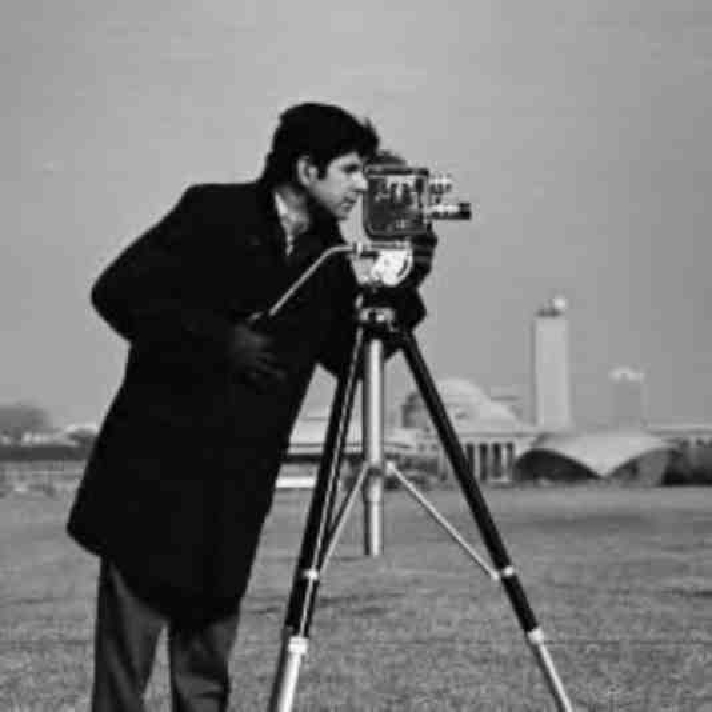
\includegraphics[width=5cm, height=5cm]{man-unmodified.jpg}
	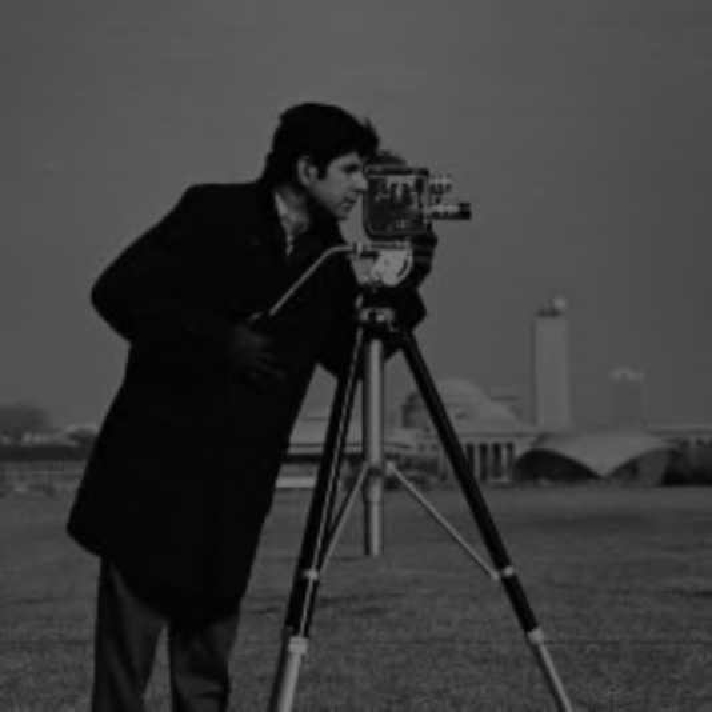
\includegraphics[width=5cm, height=5cm]{2/multiply-gray-const.png}
	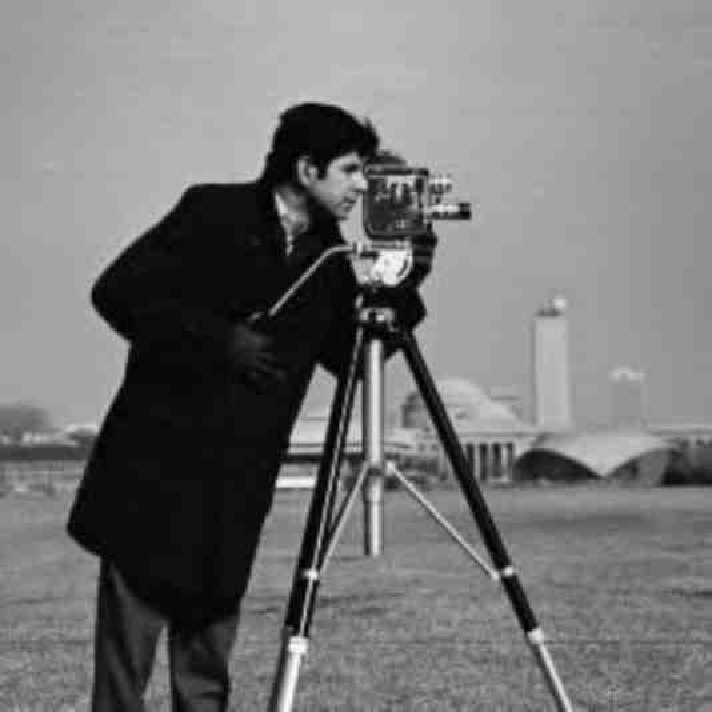
\includegraphics[width=5cm, height=5cm]{2/multiply-gray-const-norm.png}
\end{figure}
\begin{figure}[H]
	\caption{Przed uruchomieniem algorytmu (lewy obraz), po pomnożeniu przez wartość 1.5 (środkowy obraz), po normalizacji (prawy obraz)}
	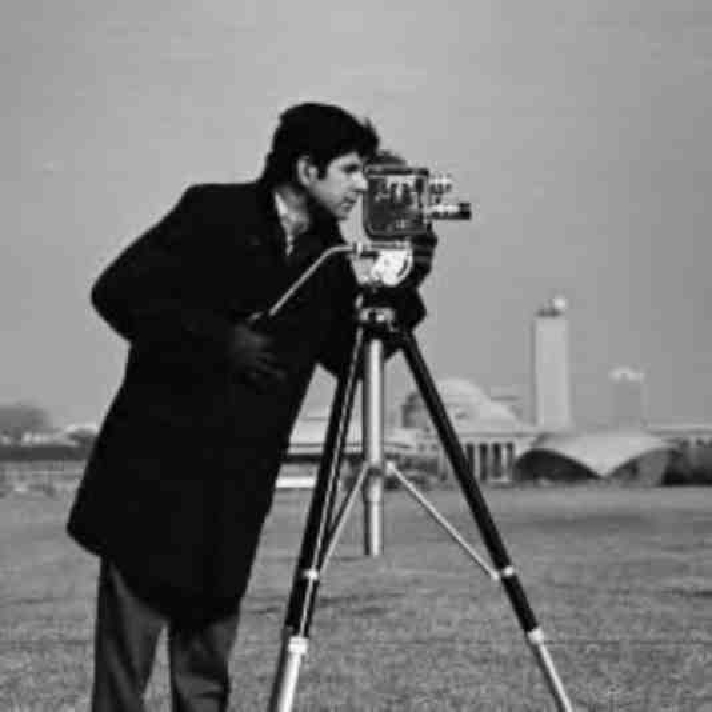
\includegraphics[width=5cm, height=5cm]{man-unmodified.jpg}
	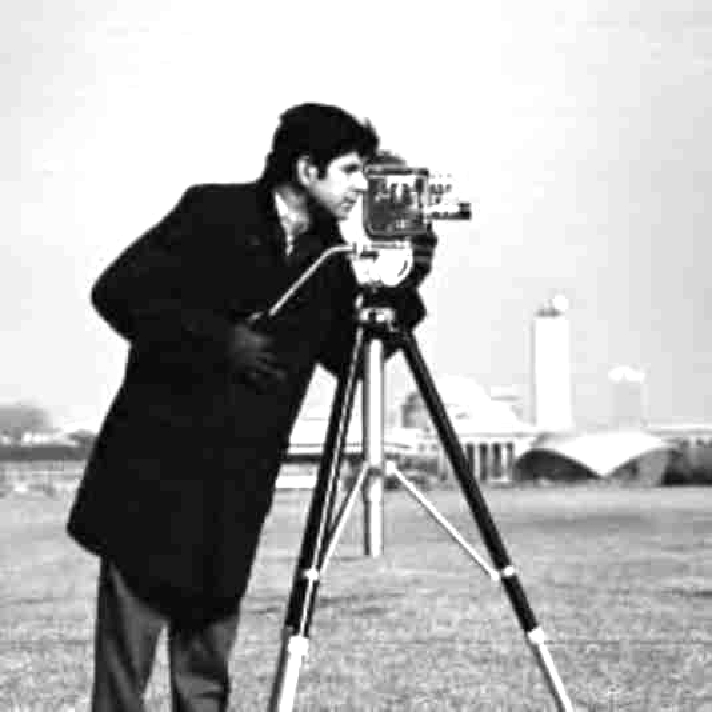
\includegraphics[width=5cm, height=5cm]{2/multiply-gray-const-2.png}
	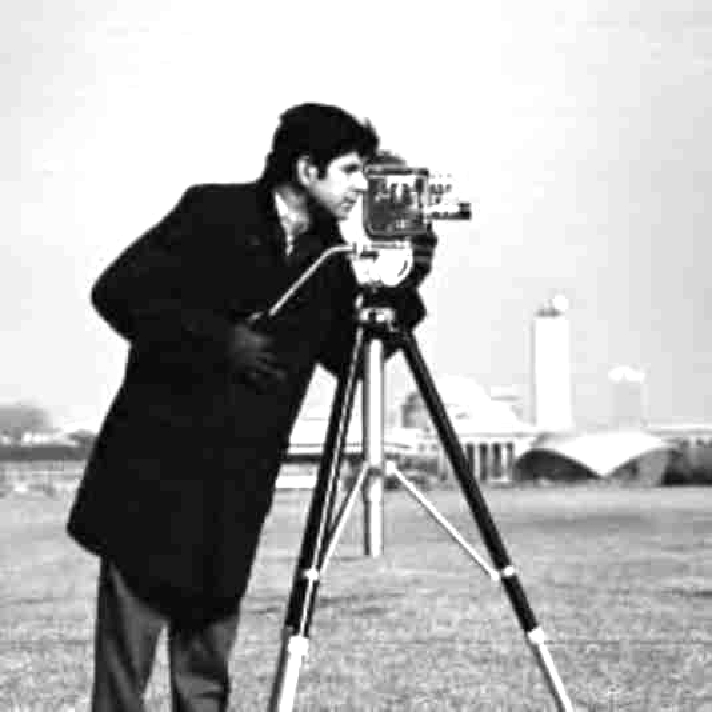
\includegraphics[width=5cm, height=5cm]{2/multiply-gray-const-2-norm.png}
\end{figure}

\begin{figure}[H]
	\caption{Przed uruchomieniem algorytmu (lewy obraz), po pomnożeniu przez wartość 0.5 (środkowy obraz), po normalizacji (prawy obraz)}
	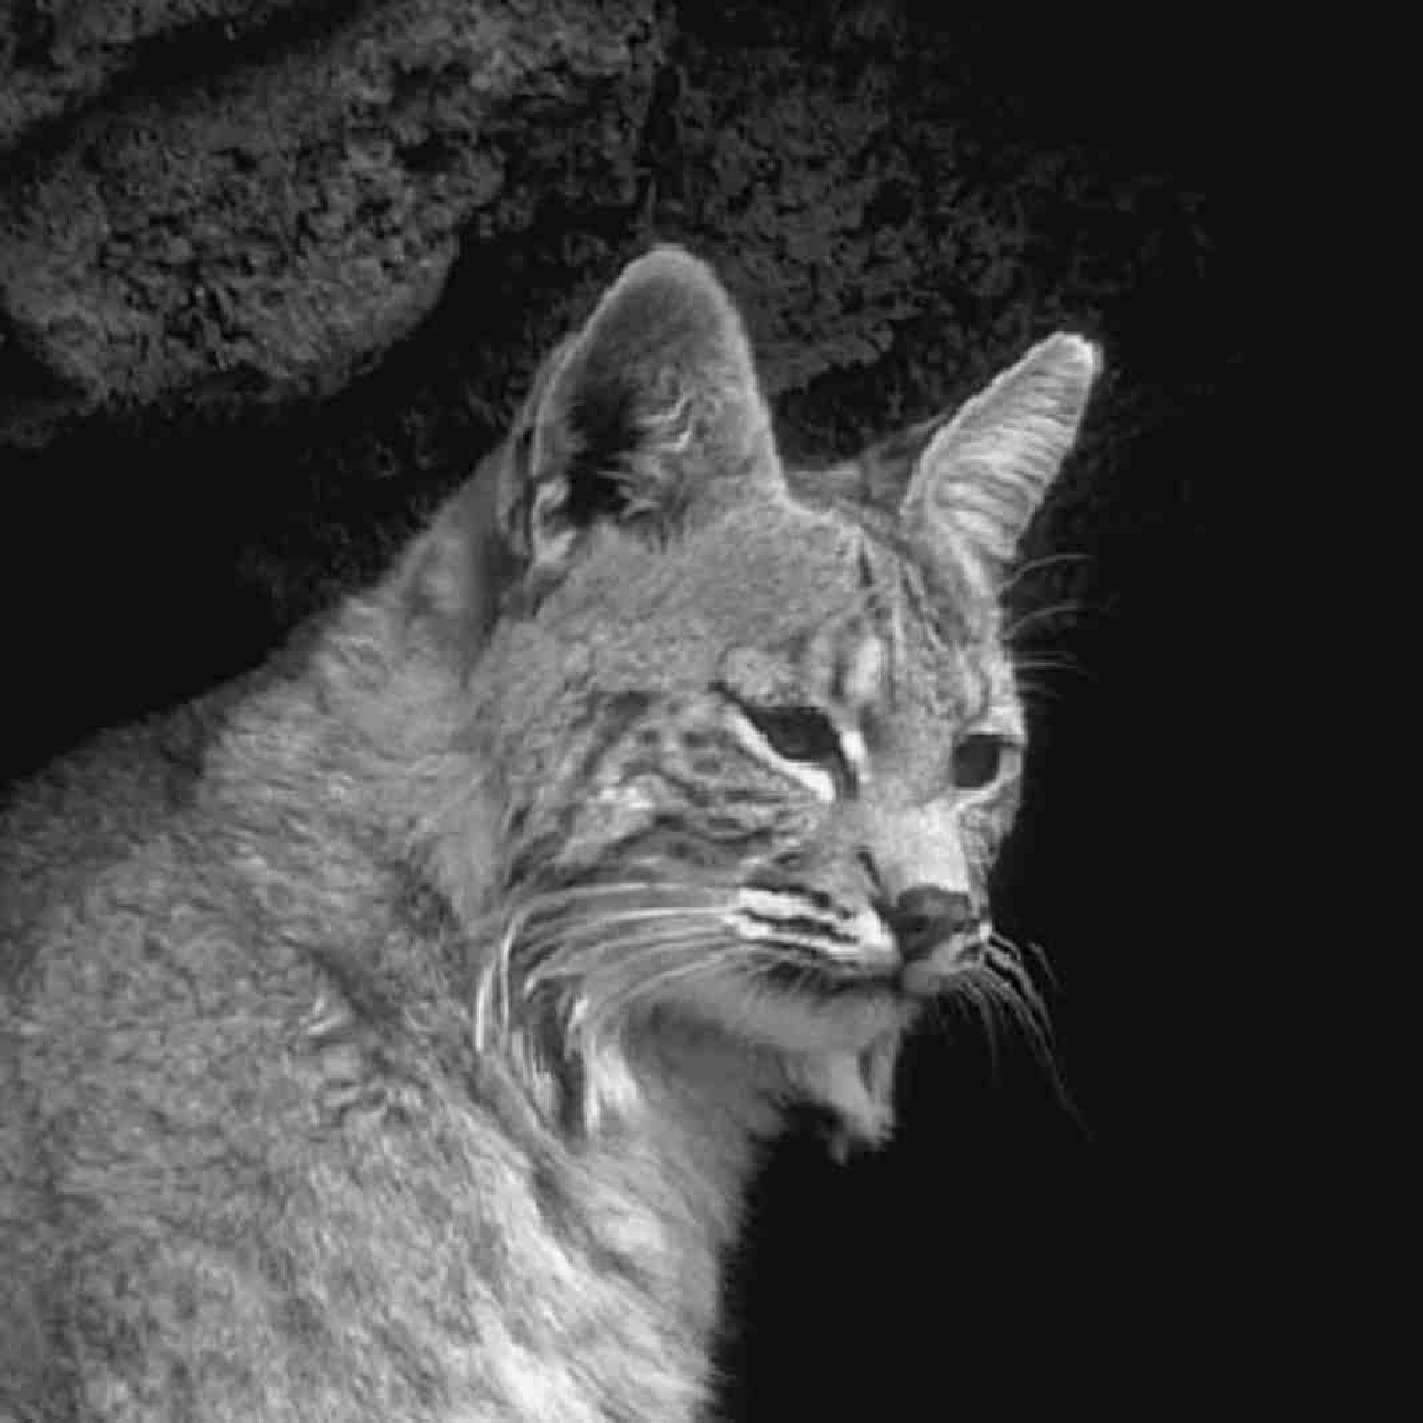
\includegraphics[width=5cm, height=5cm]{cat-unmodified.jpg}
	\includegraphics[width=5cm, height=5cm]{2/multiply-gray-const-3.png}
	\includegraphics[width=5cm, height=5cm]{2/multiply-gray-const-3-norm.png}
\end{figure}
\begin{figure}[H]
	\caption{Przed uruchomieniem algorytmu (lewy obraz), po pomnożeniu przez wartość 1.5 (środkowy obraz), po normalizacji (prawy obraz)}
	\includegraphics[width=5cm, height=5cm]{cat-unmodified.jpg}
	\includegraphics[width=5cm, height=5cm]{2/multiply-gray-const-4.png}
	\includegraphics[width=5cm, height=5cm]{2/multiply-gray-const-4-norm.png}
\end{figure}

\subsection*{Kod źródłowy programu}
\inputpython{../Source/ArithmeticSumGray.py}{63}{77}

\section{Mnożenie obrazu przez inny obraz}
\subsection*{Algorytm}
\subsubsection*{Opis}
Drugą formą mnożenia obrazu jest sytuacja gdy mnożnikiem jest inny obraz. Operacja ta przebiega analogicznie jak przy stałej, ale z tą różnicą że każdy piksel mnożymy przez odpowiadający mu piksel w drugim obrazie, zgodnie ze wzorem: 
\begin{gather}
	Q(i,j) = P_1(i,j) \times P_2(i,j)
\end{gather}
W zależności od tego jakich wartości w obrazach użyjemy otrzymamy różne rezultaty: 
\begin{enumerate}
	\item Dla dwóch obrazów, które wartości posiadają z przedziału $(0, Z_{rep})$ obrazy będą się na siebie nakładać (Rysunek 3.12 i 3.13). 
	\item Dla obrazów w których jeden z nich jest używany jako maska otrzymamy wyciętą zawartość drugiego obrazu (Rysunek 3.14). 
\end{enumerate}
Przydatną własnością tej operacji jest możliwość wyciągania części wspólnych z obrazów, dzięki czemu wykrywanie ruch na obrazach po-klatkowych jest łatwiejsze. 

\begin{figure}[H]
	\caption{Przed uruchomieniem algorytmu (obrazy na górze), po przemnożeniu obrazów (lewy, dolny obraz), po normalizacji (prawy, dolny obraz)}
	\includegraphics[width=7cm, height=7cm]{man-unmodified.jpg}
	\includegraphics[width=7cm, height=7cm]{lena-unmodified.png}
	\includegraphics[width=7cm, height=7cm]{2/multiply-gray-images-2.png}
	\includegraphics[width=7cm, height=7cm]{2/multiply-gray-images-2-norm.png}
\end{figure}
\begin{figure}[H]
	\caption{Przed uruchomieniem algorytmu (obrazy na górze), po przemnożeniu obrazów (lewy, dolny obraz), po normalizacji (prawy, dolny obraz)}
	\includegraphics[width=7cm, height=7cm]{man-unmodified.jpg}
	\includegraphics[width=7cm, height=7cm]{cat-unmodified.jpg}
	\includegraphics[width=7cm, height=7cm]{2/multiply-gray-images.png}
	\includegraphics[width=7cm, height=7cm]{2/multiply-gray-images-norm.png}
\end{figure}
\begin{figure}[H]
\caption{Przed uruchomieniem algorytmu (obrazy na górze), po przemnożeniu obrazów (lewy, dolny obraz), po normalizacji (prawy, dolny obraz)}
\includegraphics[width=7cm, height=7cm]{cat-unmodified.jpg}
\includegraphics[width=7cm, height=7cm]{mask-unmodified.png}
\includegraphics[width=7cm, height=7cm]{2/multiply-gray-images-mask.png}
\includegraphics[width=7cm, height=7cm]{2/multiply-gray-images-mask.png}
\end{figure}

\subsection*{Kod źródłowy programu}
\inputpython{../Source/ArithmeticSumGray.py}{80}{95}

\section{Mieszanie obrazów z określonym współczynnikiem}
\subsection*{Algorytm}
\subsubsection*{Opis}
Operator liniowego mieszania przyjmuje dwa obrazy tych samych rozmiarów, co wymaga skalowania geometrycznego, i zwraca liniową kombinację odpowiadających sobie pikseli (tak samo jak w przypadku dodawania). Wynikiem jest efekt przechodzenia obrazu $f$ w obraz $f^\prime$, a jego natężenie ustala się z pomocą specjalnego współczynnika. \\
Współczynnik $\alpha$ jest wartością określaną przez użytkownika z zakresu $[0,1]$. Jego zadaniem jest skalowanie wartości każdego piksela w obu obrazach przed ich połączeniem, dzięki czemu raz mogą być faworyzowane wartości z $f^\prime$ i raz z $f$. \\
Do obliczeń operatora będzie używany wzór: 
\begin{gather}
	f_{result}(i,j) = \alpha \times f(i,j) + (1 - \alpha) \times f^\prime(i,j)
\end{gather}
Wadą mieszania względem dodawania obrazów jest sam proces skalowania wartości pikseli, który sprawia, że przy wybraniu zbyt małej wartości $\alpha$ kontrast między pikselami jest zatracany. Problem występuje głównie, gdy kontrast na samych obrazach jest dość ubogi. Aby podtrzymać kontrast możemy zwiększyć współczynnik $\alpha$ lub zdefiniować odpowiednią maskę dla naszego obrazu. Maska $f_m$ jest rozmiaru $f_{result}$ i składa się z wartości z zakresu $[0, Z_p]$. Każda wartość takiej maski odpowiada współczynnikowi $\alpha$ dla każdego piksela w $f$ i $f^\prime$. Wzór wygląda wtedy tak: 
\begin{gather}
	f_{result}(i,j) = \frac{f_m(i,j)}{Z_p} \times f(i,j) + (1 - \frac{f_m(i,j)}{Z_p}) \times f^\prime(i,j)
\end{gather}
\begin{figure}[H]
	\caption{Przed uruchomieniem algorytmu}
	\includegraphics[width=8cm, height=8cm]{man-unmodified.jpg}
	\includegraphics[width=8cm, height=8cm]{lena-unmodified.png}
\end{figure}
\begin{figure}[H]
	\caption{Po mieszaniu o wartość 0.2 (lewy obraz), po mieszaniu o wartość 0.5 (środkowy obraz), po mieszaniu o wartość 0.8 (prawy obraz)}
	\includegraphics[width=5cm, height=5cm]{2/blend-gray-images-2.png}
	\includegraphics[width=5cm, height=5cm]{2/blend-gray-images-5.png}
	\includegraphics[width=5cm, height=5cm]{2/blend-gray-images-8.png}
\end{figure}

\subsection*{Kod źródłowy programu}
\inputpython{../Source/ArithmeticSumGray.py}{98}{114}

\section{Potęgowanie obrazu z zadaną potęgą}
\subsection*{Algorytm}
\subsubsection*{Opis}
Efektem operatora potęgowania jest zmniejszenie lub zwiększenie kontrastu pomiędzy pikselami. W przeciwieństwie do operacji dodawania, która zmniejszała lub zwiększała wartość wszystkich pikseli, potęgowanie wpływa na odległość pomiędzy wartościami na osi. Zachowanie wynika z własności funkcji wykładniczej (Rysunek 3.16) - im mniejsza wartość bazowa tym wolniejszy przyrost, a dla większych szybszy przyrost. 
\begin{figure}[H]
	\caption{Wykres eksponenty}
	\includegraphics[width=10cm, height=10cm]{overview/exponential-curve.png}
\end{figure}
W zależności od dobrania odpowiedniej wartości \textit{wykładnika} możemy: 
\begin{enumerate}
	\item zwiększyć kontrast dla małych jaskrawości; wybierając $\alpha \in (0,1)$. 
	\item zwiększyć kontrast dla dużych jaskrawości; wybierając $\alpha \in (1,\infty)$. 
\end{enumerate}
Obliczając wartości pikseli użyjemy wzoru: 
\begin{gather}
	f_m = f^\alpha
\end{gather}
Po wykonaniu tej operacji będzie potrzebne zastosowanie normalizacji do uwidocznienie wyników. 

\begin{figure}[H]
	\caption{Przed uruchomieniem algorytmu (lewy obraz), po użyciu potęgowania o wykładniku 0.5 (środkowy obraz), po normalizacji (prawy obraz)}
	\includegraphics[width=5cm, height=5cm]{man-unmodified.jpg}
	\includegraphics[width=5cm, height=5cm]{2-4/power-gray-photoman-5.png}
	\includegraphics[width=5cm, height=5cm]{2-4/power-gray-photoman-5-norm.png}
\end{figure}
\begin{figure}[H]
	\caption{Przed uruchomieniem algorytmu (lewy obraz), po użyciu potęgowania o wykładniku 2 (środkowy obraz), po normalizacji (prawy obraz)}
	\includegraphics[width=5cm, height=5cm]{man-unmodified.jpg}
	\includegraphics[width=5cm, height=5cm]{2-4/power-gray-photoman-20.png}
	\includegraphics[width=5cm, height=5cm]{2-4/power-gray-photoman-20-norm.png}
\end{figure}
\begin{figure}[H]
\caption{Przed uruchomieniem algorytmu (lewy obraz), po użyciu potęgowania o wykładniku 0.5 (środkowy obraz), po normalizacji (prawy obraz)}
\includegraphics[width=5cm, height=5cm]{cat-unmodified.jpg}
\includegraphics[width=5cm, height=5cm]{2-4/power-gray-cat-5.png}
\includegraphics[width=5cm, height=5cm]{2-4/power-gray-cat-5-norm.png}
\end{figure}
\begin{figure}[H]
\caption{Przed uruchomieniem algorytmu (lewy obraz), po użyciu potęgowania o wykładniku 2 (środkowy obraz), po normalizacji (prawy obraz)}
\includegraphics[width=5cm, height=5cm]{cat-unmodified.jpg}
\includegraphics[width=5cm, height=5cm]{2-4/power-gray-cat-20.png}
\includegraphics[width=5cm, height=5cm]{2-4/power-gray-cat-20-norm.png}
\end{figure}

\subsection*{Kod źródłowy programu}
\inputpython{../Source/ArithmeticSumGray.py}{117}{130}

\chapter{Operacje sumowania arytmetycznego obrazów barwowych}
Rodzaje operatorów arytmetycznych używane na obrazach barwowych różnią się względem ich szarych odpowiedników tylko strukturą na której pracują. Piksel obrazów szarych składa się z jednej wartości z zakresu $[0,255]$. W przypadku kolorowych obrazów potrzebne są trzy wartości na każdą barwę \textit{RGB}. 
\\
Funkcja normalizacji w przypadku tego rodzaju obrazu wygląda tak: 
\inputpython{../Source/Commons.py}{8}{15}
Pobiera ona informacje o maksymalnej dostępnej wartości dla kanału piksela $maxValue$ (w tym wypadku 255). Po czym wśród wszystkich pikselach i ich składowych znajduje najmniejszą i największą wartość $fmin$ i $fmax$. Następnie wykonywane są obliczenia mające na celu przeskalowanie wartości do innego przedziału. W wypadku gdy $fmin$ i $fmax$ znajdują się niedaleko od siebie, normalizacja zapewni aby wartości obrazu wynikowego będą rozpięte na przedział $[0,255]$ z $fmin$ i $fmax$, który może być mniejszy (np z zakresu $[50,90]$). Dzięki temu zabiegowi proporcje między barwami zostaną zachowane i obraz ożywi się trochę kolorami. 

\section{Sumowanie (określonej) stałej z obrazem}
\subsection*{Algorytm}
\subsubsection*{Opis}
\begin{figure}[H]
	\caption{Przed uruchomieniem algorytmu (lewy obraz), po użyciu dodawania o wartości 30 (środkowy obraz), po normalizacji (prawy obraz)}
	\includegraphics[width=5cm, height=5cm]{coffee-unmodified.jpg}
	\includegraphics[width=5cm, height=5cm]{3-1/sum-color-const-coffee-30.png}
	\includegraphics[width=5cm, height=5cm]{3-1/sum-color-const-coffee-30-norm.png}
\end{figure}
\begin{figure}[H]
\caption{Przed uruchomieniem algorytmu (lewy obraz), po użyciu dodawania o wartości 30 (środkowy obraz), po normalizacji (prawy obraz)}
\includegraphics[width=5cm, height=5cm]{phone-unmodified.jpg}
\includegraphics[width=5cm, height=5cm]{3-1/sum-color-const-phone-30.png}
\includegraphics[width=5cm, height=5cm]{3-1/sum-color-const-phone-30-norm.png}
\end{figure}
\begin{figure}[H]
\caption{Przed uruchomieniem algorytmu (lewy obraz), po użyciu dodawania o wartości 200 (środkowy obraz), po normalizacji (prawy obraz)}
\includegraphics[width=5cm, height=5cm]{coffee-unmodified.jpg}
\includegraphics[width=5cm, height=5cm]{3-1/sum-color-const-coffee-200.png}
\includegraphics[width=5cm, height=5cm]{3-1/sum-color-const-coffee-200-norm.png}
\end{figure}
\begin{figure}[H]
\caption{Przed uruchomieniem algorytmu (lewy obraz), po użyciu dodawania o wartości 200 (środkowy obraz), po normalizacji (prawy obraz)}
\includegraphics[width=5cm, height=5cm]{phone-unmodified.jpg}
\includegraphics[width=5cm, height=5cm]{3-1/sum-color-const-phone-200.png}
\includegraphics[width=5cm, height=5cm]{3-1/sum-color-const-phone-200-norm.png}
\end{figure}

\subsection*{Kod źródłowy programu}
\inputpython{../Source/ArithmeticSumColor.py}{18}{37}

\section{Sumowanie dwóch obrazów}
\subsection*{Algorytm}
\subsubsection*{Opis}
\begin{figure}[H]
	\caption{Przed (obrazy na górze), po dodaniu obrazów (lewy, dolny obraz), po normalizacji (prawy, dolny obraz)}
	\includegraphics[width=7cm, height=7cm]{coffee-unmodified.jpg}
	\includegraphics[width=7cm, height=7cm]{phone-unmodified.jpg}
	\includegraphics[width=7cm, height=7cm]{3-1/sum-color-images-coffee-phone.png}
	\includegraphics[width=7cm, height=7cm]{3-1/sum-color-images-coffee-phone-norm.png}
\end{figure}
\begin{figure}[H]
	\caption{Przed (obrazy na górze), po dodaniu obrazów (lewy, dolny obraz), po normalizacji (prawy, dolny obraz)}
	\includegraphics[width=7cm, height=7cm]{phone-unmodified.jpg}
	\includegraphics[width=7cm, height=7cm]{sea-unmodified.jpg}
	\includegraphics[width=7cm, height=7cm]{3-1/sum-color-images-phone-sea.png}
	\includegraphics[width=7cm, height=7cm]{3-1/sum-color-images-phone-sea-norm.png}
\end{figure}

\subsection*{Kod źródłowy programu}
\inputpython{../Source/ArithmeticSumColor.py}{40}{63}

\section{Mnożenie obrazu przez zadaną liczbę}
\subsection*{Algorytm}
\subsubsection*{Opis}
\begin{figure}[H]
	\caption{Przed (lewy obraz), po pomnożeniu przez wartości 0.5 (środkowy obraz), po normalizacji (prawy obraz)}
	\includegraphics[width=5cm, height=5cm]{coffee-unmodified.jpg}
	\includegraphics[width=5cm, height=5cm]{3-2/multiply-color-const-coffee-5.png}
	\includegraphics[width=5cm, height=5cm]{3-2/multiply-color-const-coffee-5-norm.png}
\end{figure}
\begin{figure}[H]
	\caption{Przed (lewy obraz), po pomnożeniu przez wartości 0.5 (środkowy obraz), po normalizacji (prawy obraz)}
	\includegraphics[width=5cm, height=5cm]{phone-unmodified.jpg}
	\includegraphics[width=5cm, height=5cm]{3-2/multiply-color-const-phone-5.png}
	\includegraphics[width=5cm, height=5cm]{3-2/multiply-color-const-phone-5-norm.png}
\end{figure}
\begin{figure}[H]
	\caption{Przed (lewy obraz), po pomnożeniu przez wartości 1.5 (środkowy obraz), po normalizacji (prawy obraz)}
	\includegraphics[width=5cm, height=5cm]{coffee-unmodified.jpg}
	\includegraphics[width=5cm, height=5cm]{3-2/multiply-color-const-coffee-15.png}
	\includegraphics[width=5cm, height=5cm]{3-2/multiply-color-const-coffee-15-norm.png}
\end{figure}
\begin{figure}[H]
	\caption{Przed (lewy obraz), po pomnożeniu przez wartości 1.5 (środkowy obraz), po normalizacji (prawy obraz)}
	\includegraphics[width=5cm, height=5cm]{phone-unmodified.jpg}
	\includegraphics[width=5cm, height=5cm]{3-2/multiply-color-const-phone-15.png}
	\includegraphics[width=5cm, height=5cm]{3-2/multiply-color-const-phone-15-norm.png}
\end{figure}

\subsection*{Kod źródłowy programu}
\inputpython{../Source/ArithmeticSumColor.py}{67}{85}

\section{Mnożenie obrazu przez inny obraz}
\subsection*{Algorytm}
\subsubsection*{Opis}
\begin{figure}[H]
	\caption{Przed (górne obrazy), po pomnożeniu obrazów (lewy, dolny obraz), po normalizacji (prawy, dolny obraz)}
	\includegraphics[width=7cm, height=7cm]{coffee-unmodified.jpg}
	\includegraphics[width=7cm, height=7cm]{phone-unmodified.jpg}
	\includegraphics[width=7cm, height=7cm]{3-2/multiply-color-images-coffee-phone.png}
	\includegraphics[width=7cm, height=7cm]{3-2/multiply-color-images-coffee-phone-norm.png}
\end{figure}
\begin{figure}[H]
	\caption{Przed (górne obrazy), po pomnożeniu obrazów (lewy, dolny obraz), po normalizacji (prawy, dolny obraz)}
	\includegraphics[width=7cm, height=7cm]{phone-unmodified.jpg}
	\includegraphics[width=7cm, height=7cm]{sea-unmodified.jpg}
	\includegraphics[width=7cm, height=7cm]{3-2/multiply-color-images-phone-sea.png}
	\includegraphics[width=7cm, height=7cm]{3-2/multiply-color-images-phone-sea-norm.png}
\end{figure}

\subsection*{Kod źródłowy programu}
\inputpython{../Source/ArithmeticSumColor.py}{88}{104}

\section{Mieszanie obrazów z określonym współczynnikiem}
\subsection*{Algorytm}
\subsubsection*{Opis}
\begin{figure}[H]
	\caption{Przed uruchomieniem algorytmu}
	\includegraphics[width=8cm, height=8cm]{coffee-unmodified.jpg}
	\includegraphics[width=8cm, height=8cm]{phone-unmodified.jpg}
\end{figure}
\begin{figure}[H]
	\caption{Po mieszaniu o wartość 0.2 (lewy obraz), po mieszaniu o wartość 0.5 (środkowy obraz), po mieszaniu o wartość 0.8 (prawy obraz)}
	\includegraphics[width=5cm, height=5cm]{3-3/blend-color-images-coffee-2.png}
	\includegraphics[width=5cm, height=5cm]{3-3/blend-color-images-coffee-5.png}
	\includegraphics[width=5cm, height=5cm]{3-3/blend-color-images-coffee-8.png}
\end{figure}

\subsection*{Kod źródłowy programu}
\inputpython{../Source/ArithmeticSumColor.py}{107}{124}

\section{Potęgowanie obrazu (z zadaną potęgą)}
\subsection*{Algorytm}
\subsubsection*{Opis}
\begin{figure}[H]
	\caption{Przed uruchomieniem algorytmu (lewy obraz), po użyciu potęgowania o wykładniku 0.5 (środkowy obraz), po normalizacji (prawy obraz)}
	\includegraphics[width=5cm, height=5cm]{coffee-unmodified.jpg}
	\includegraphics[width=5cm, height=5cm]{3-4/power-color-coffee-5.png}
	\includegraphics[width=5cm, height=5cm]{3-4/power-color-coffee-5-norm.png}
\end{figure}
\begin{figure}[H]
	\caption{Przed uruchomieniem algorytmu (lewy obraz), po użyciu potęgowania o wykładniku 2 (środkowy obraz), po normalizacji (prawy obraz)}
	\includegraphics[width=5cm, height=5cm]{coffee-unmodified.jpg}
	\includegraphics[width=5cm, height=5cm]{3-4/power-color-coffee-2.png}
	\includegraphics[width=5cm, height=5cm]{3-4/power-color-coffee-2-norm.png}
\end{figure}
\begin{figure}[H]
	\caption{Przed uruchomieniem algorytmu (lewy obraz), po użyciu potęgowania o wykładniku 0.5 (środkowy obraz), po normalizacji (prawy obraz)}
	\includegraphics[width=5cm, height=5cm]{phone-unmodified.jpg}
	\includegraphics[width=5cm, height=5cm]{3-4/power-color-phone-5.png}
	\includegraphics[width=5cm, height=5cm]{3-4/power-color-phone-5-norm.png}
\end{figure}
\begin{figure}[H]
	\caption{Przed uruchomieniem algorytmu (lewy obraz), po użyciu potęgowania o wykładniku 2 (środkowy obraz), po normalizacji (prawy obraz)}
	\includegraphics[width=5cm, height=5cm]{phone-unmodified.jpg}
	\includegraphics[width=5cm, height=5cm]{3-4/power-color-phone-2.png}
	\includegraphics[width=5cm, height=5cm]{3-4/power-color-phone-2-norm.png}
\end{figure}

\subsection*{Kod źródłowy programu}
\inputpython{../Source/ArithmeticSumColor.py}{127}{142}

\chapter{Operacje geometryczne na obrazie}
Operacje geometryczne przekształcają położenie pikseli \textit{(x1, y1)} w obrazie wejściowym do nowej lokacji \textit{(x2, y2)} w obrazie wynikowym. Dzięki temu możemy dopasować obraz do odpowiedniego układu współrzędnych lub użyć tych operacji do eliminacji geometrycznych zakłóceń obrazu (dystorsji). 
\section{Przemieszczenie obrazu o zadany wektor}
\subsection*{Opis}
Operacja translacji wykonuje transformację geometryczną polegającą na przeniesieniu każdego z punktów obrazu wejściowego w nowe miejsce na obrazie wynikowym. Pod wpływem translacji element obrazu zlokalizowany na \textit{(x1, y1)} zostanie przesunięty na nową pozycję \textit{(x2, y2)}. Różnicą pomiędzy \textit{(x1, y1)} i \textit{(x2, y2)} jest wektor \textit{(bx, by)}, który jest określony przez użytkownika. 
\newline
Operacja przemieszczenia przybiera postać: 
\begin{gather}
	x_2 = x_1 + b_x \\
	y_2 = y_1 + b_y
\end{gather}
\begin{figure}[H]
	\caption{Przed uruchomieniem algorytmu (lewy obraz), po przesunięciu o wektor [100, 100] (prawy obraz)}
	\includegraphics[width=8cm, height=8cm]{phone-unmodified.jpg}
	\includegraphics[width=8cm, height=8cm]{phone-translate.png}
\end{figure}
\begin{figure}[H]
	\caption{Przed uruchomieniem algorytmu (lewy obraz), po przesunięciu o wektor [100, -100] (prawy obraz)}
	\includegraphics[width=8cm, height=8cm]{coffee-unmodified.jpg}
	\includegraphics[width=8cm, height=8cm]{coffee-translate.png}
\end{figure}
\subsection*{Kod źródłowy algorytmu}
\begin{python}
def translate(self, deltaX = 0, deltaY = 0):
	print('translation start')
	height, width = self.decoder.height, self.decoder.width
	image = self.decoder.getPixels24Bits()
	result = numpy.zeros((height, width, 3), numpy.uint8)
	
	for y in range(height):
		for x in range(width):  
			if 0 < y + deltaY < height and 0 < x + deltaX < width:
				result[y + deltaY][x + deltaX] = image[y][x]
	
	img = Image.fromarray(result, mode='RGB')
	img.save('Resources/tGeometric.png')
print('translation done')
\end{python}
\section{Jednorodne skalowanie obrazu}
\subsection*{Opis}
Skalowanie jednorodne obrazu składa się na pomnożenie współrzędnych każdego piksela przez określoną wartość. 
\begin{gather}
x_2 = S_x * x_1 \\
y_2 = S_y * y_1
\end{gather}
Przy czym skalowanie jednorodne oznacza, że po zmianie wartości współrzędnych nasz obraz zachowa dawne proporcje. Czyli: 
\begin{gather}
S_x = S_y
\end{gather}
\begin{figure}[H]
	\caption{Przed uruchomieniem algorytmu (lewy obraz), po skalowaniu jednorodnym o współczynnik 2 (prawy obraz)}
	\includegraphics[width=4cm, height=4cm]{coffee-unmodified.jpg}
	\includegraphics[width=4cm, height=4cm]{coffee-hscaling-without-interpolation.png}
	\includegraphics[width=4cm, height=4cm]{coffee-hscaling.png}
\end{figure}
\subsection*{Kod źródłowy algorytmu}
\begin{python}
def homogeneousScaling(self, scale = 1.0):
	print('homogeneous scaling start')
	image = self.decoder.getPixels24Bits()
	
	print('scaling')
	result = self._scaleXY(image, scale)
	print('interpolation')
	self._interpolateColor(result)
	
	img = Image.fromarray(result, mode='RGB')
	img.save('Resources/hsGeometric.png')
	print('homogeneous scaling done')

def _scaleXY(self, matrix, scale):
	height, width = self.decoder.height, self.decoder.width
	result = numpy.full((height, width, 3), 1, numpy.uint8)
	for y in range(height):
		for x in range(width):  
			if scale * y < height and scale * x < width:
				result[int(scale * y)][int(scale * x)] = matrix[y][x]
	return result

def _interpolateColor(self, result):
	height, width = self.decoder.height, self.decoder.width
	for h in range(height):
		for w in range(width):
			r, g, b = 0, 0, 0
			n = 0
			if (result[h, w][0] == 1) & (result[h, w][1] == 1) & (result[h, w][2] == 1):
				for hOff in range(-1, 2):
					for wOff in range(-1, 2):
						hSafe = h if ((h + hOff) > (height - 2)) | ((h + hOff) < 0) else (h + hOff)
						wSafe = w if ((w + wOff) > (width - 2)) | ((w + wOff) < 0) else (w + wOff)
						if (result[hSafe, wSafe][0] > 1) | (result[hSafe, wSafe][1] > 1) | (result[hSafe, wSafe][2] > 1):
							r += result[hSafe, wSafe][0]
							g += result[hSafe, wSafe][1]
							b += result[hSafe, wSafe][2]
							n += 1
				result[h, w] = (r/n, g/n, b/n)
\end{python}
\section{Niejednorodne skalowanie obrazu}
\subsection*{Opis}
Skalowanie niejednorodne obrazu składa się na pomnożenie współrzędnych każdego piksela przez określoną wartość. 
\begin{gather}
x_2 = S_x * x_1 \\
y_2 = S_y * y_1
\end{gather}
Przy czym skalowanie niejednorodne oznacza, że po zmianie wartości współrzędnych nasz obraz będzie miał zachwiane proporcje. Czyli: 
\begin{gather}
S_x \neq S_y
\end{gather}
\begin{figure}[H]
	\caption{Przed uruchomieniem algorytmu (lewy obraz), po skalowaniu jednorodnym o współczynnik x = 2.0, y = 1.0 (prawy obraz)}
	\includegraphics[width=4cm, height=4cm]{coffee-unmodified.jpg}
	\includegraphics[width=4cm, height=4cm]{coffee-nonuniform-scaling-without-interpolation.png}
	\includegraphics[width=4cm, height=4cm]{coffee-nonuniform-scaling.png}
\end{figure}
\subsection*{Kod źródłowy algorytmu}
\begin{python}
def nonUniformScaling(self, scaleX = 1.0, scaleY = 1.0):
	print('non-uniform scaling start')
	image = self.decoder.getPixels24Bits()
	
	print('scaling')
	result = self._scale(image, scaleX, scaleY)
	print('interpolation')
	self._interpolateColor(result)
	
	img = Image.fromarray(result, mode='RGB')
	img.save('Resources/nusGeometric.png')
	print('non-uniform scaling done')

def _scale(self, matrix, scaleX, scaleY):
	height, width = self.decoder.height, self.decoder.width
	result = numpy.full((height, width, 3), 1, numpy.uint8)
	for y in range(height):
		for x in range(width):  
			if scaleY * y < height and scaleX * x < width:
				result[int(scaleY * y)][int(scaleX * x)] = matrix[y][x]
	return result

def _interpolateColor(self, result):
	height, width = self.decoder.height, self.decoder.width
	for h in range(height):
		for w in range(width):
			r, g, b = 0, 0, 0
			n = 0
				if (result[h, w][0] == 1) & (result[h, w][1] == 1) & (result[h, w][2] == 1):
					for hOff in range(-1, 2):
						for wOff in range(-1, 2):
							hSafe = h if ((h + hOff) > (height - 2)) | ((h + hOff) < 0) else (h + hOff)
							wSafe = w if ((w + wOff) > (width - 2)) | ((w + wOff) < 0) else (w + wOff)
							if (result[hSafe, wSafe][0] > 1) | (result[hSafe, wSafe][1] > 1) | (result[hSafe, wSafe][2] > 1):
								r += result[hSafe, wSafe][0]
								g += result[hSafe, wSafe][1]
								b += result[hSafe, wSafe][2]
								n += 1
						result[h, w] = (r/n, g/n, b/n)
\end{python}
\section{Obracanie obrazu o dowolny kąt}
\subsection*{Opis}
Operacja obrotu wykonywana jest wokół początku układu współrzędnych o kąt $\varphi$ w taki sposób aby odległość od początku układu do punktu pozostała bez zmian, oraz aby pomiędzy odcinkami danych punków był kąt $\varphi$. Właściwości te można pozyskać dzięki wzorom: 
\begin{gather}
	x` = x\cos(\varphi) - y\sin(\varphi) \\
	y` = x\sin(\varphi) + y\cos(\varphi)
\end{gather}
gdzie \textit{(x`, y`)} to nowe współrzędne wyznaczone po obrocie punktu \textit{(x, y)} o kąt $\varphi$. 
\begin{figure}[H]
	\caption{Przed uruchomieniem algorytmu (lewy obraz), po obróceniu o kąt $45^o$(prawy obraz), po obrocie bez interpolacji (środkowy obraz)}
	\includegraphics[width=4cm, height=4cm]{sea-unmodified.jpg}
	\includegraphics[width=4cm, height=4cm]{sea-rotation-without-interpolation.png}
	\includegraphics[width=4cm, height=4cm]{sea-rotation.png}
\end{figure}
\subsection*{Kod źródłowy algorytmu}
\begin{python}
def rotation(self, phi):
	print('rotation start')
	image = self.decoder.getPixels24Bits()
	
	print('rotating')
	result = self._rotate(image, phi)
	print('interpolation')
	self._interpolateColor(result)
	
	img = Image.fromarray(result, mode='RGB')
	img.save('Resources/rGeometric.png')
	print('rotation done')

def _rotate(self, image, phi):
	height, width = self.decoder.height, self.decoder.width
	result = numpy.full((height, width, 3), 1, numpy.uint8)
	radian = math.radians(phi)
	for y in range(height):
		for x in range(width): 
			newX = x*math.cos(radian) - y*math.sin(radian)
			newY = x*math.sin(radian) + y*math.cos(radian)
			if newY < height and newY >= 0 and newX >= 0 and newX < width:
				result[int(newY)][int(newX)] = image[y][x]
	return result

def _interpolateColor(self, result):
	height, width = self.decoder.height, self.decoder.width
	for h in range(height):
		for w in range(width):
			r, g, b = 0, 0, 0
			n = 0
			if (result[h, w][0] == 1) & (result[h, w][1] == 1) & (result[h, w][2] == 1):
				for hOff in range(-1, 2):
					for wOff in range(-1, 2):
						hSafe = h if ((h + hOff) > (height - 2)) | ((h + hOff) < 0) else (h + hOff)
						wSafe = w if ((w + wOff) > (width - 2)) | ((w + wOff) < 0) else (w + wOff)
						if (result[hSafe, wSafe][0] > 0) | (result[hSafe, wSafe][1] > 0) | (result[hSafe, wSafe][2] > 0):
							r += result[hSafe, wSafe][0]
							g += result[hSafe, wSafe][1]
							b += result[hSafe, wSafe][2]
							n += 1
				result[h, w] = (r/n, g/n, b/n)
\end{python}
\section{Symetrie względem osi układu}
\subsection*{Opis}
Symetria osiowa względem osi OX lub OY sprawia, że punkt \textit{(x, y)} zmienia się w \textit{(x, -y)} lub \textit{(-x, y)} w zależności czy symetria dotyczyła osi OX lub OY. W naszej pracy przyjmujemy, że lewa dolna krawędź obrazu znajduje się w punkcie \textit{(0, 0)}. 
\begin{figure}[H]
	\caption{Od lewej: przed uruchomieniem algorytmu, po symetrii względem OX, po symetrii względem OY, po symetrii względem OX oraz OY}
	\includegraphics[width=7cm, height=7cm]{sea-unmodified.jpg}
	\includegraphics[width=7cm, height=7cm]{sea-symmetry-x.png}
	\includegraphics[width=7cm, height=7cm]{sea-symmetry-y.png}
	\includegraphics[width=7cm, height=7cm]{sea-symmetry-xy.png}
\end{figure}
\subsection*{Kod źródłowy algorytmu}
\begin{python}
def axisSymmetry(self, ox, oy):
	print('axis symmetry start')
	image = self.decoder.getPixels24Bits()
	
	print('symmetry operation')
	result = self._symmetryOXorOY(image, ox, oy)
	
	img = Image.fromarray(result, mode='RGB')
	img.save('Resources/Geometric-AxisSymmetry.png')
	print('axis symmetry done')

def _symmetryOXorOY(self, image, ox, oy):
	height, width = self.decoder.height, self.decoder.width
	result = numpy.zeros((height, width, 3), numpy.uint8)
	for y in range(height):
		for x in range(width): 
			if ox and not oy:
				result[y][x] = image[y][(width-1)-x]
			elif not ox and oy:
				result[y][x] = image[(height-1)-y][x]
			elif ox and oy:
				result[y][x] = image[(height-1)-y][(width-1)-x]
	return result
\end{python}
\section{Symetrie względem zadanej prostej}
\subsection*{Opis}
Przypadek podobny do poprzedniego, lecz tym razem użytkownik podaje wiersz lub kolumnę względem której będzie przebiegała oś symetrii. 
\begin{figure}[H]
	\caption{Przed uruchomieniem algorytmu (lewy), po symetrii względem prostej \textit{x=356} (środkowy), po symetrii względem prostej \textit{y=356} (prawy)}
	\includegraphics[width=4cm, height=4cm]{phone-unmodified.jpg}
	\includegraphics[width=4cm, height=4cm]{phone-custom-symmetry-x.png}
	\includegraphics[width=4cm, height=4cm]{phone-custom-symmetry-y.png}
\end{figure}
\subsection*{Kod źródłowy algorytmu}
\begin{python}
def customSymmetryX(self, ox):
	print('custom axis symmetry X start')
	if not self._validateSymmetryAxisX(ox):
		return
	
	print('symmetry operation X')
	image = self.decoder.getPixels24Bits()
	height, width = self.decoder.height, self.decoder.width
	resultWidth = ox*2
	result = numpy.zeros((height, resultWidth, 3), numpy.uint8)
	for y in range(height):
		for x in range(ox):
			result[y][x] = image[y][x]
			result[y][resultWidth-1-x] = image[y][x]
	
	img = Image.fromarray(result, mode='RGB')
	img.save('Resources/Geometric-CustomSymmetryX.png')
	print('custom axis symmetry X done')
	
def _validateSymmetryAxisX(self, ox):
	width = self.decoder.width
	if ox <= 0 or ox > width:
		return False
	return True
	
def customSymmetryY(self, oy):
	print('custom axis symmetry Y start')
	if not self._validateSymmetryAxisY(oy):
	return
	
	print('symmetry operation Y')
	image = self.decoder.getPixels24Bits()
	height, width = self.decoder.height, self.decoder.width
	resultHeight = oy*2
	result = numpy.zeros((resultHeight, width, 3), numpy.uint8)
	for y in range(oy):
		for x in range(width):
			result[y][x] = image[y][x]
			result[resultHeight-1-y][x] = image[y][x]
	
	img = Image.fromarray(result, mode='RGB')
	img.save('Resources/Geometric-CustomSymmetryY.png')
	print('custom axis symmetry Y done')
	
def _validateSymmetryAxisY(self, oy):
	height = self.decoder.height
	if oy <= 0 or oy > height:
		return False
	return True
\end{python}
\section{Wycinanie fragmentów obrazu}
\subsection*{Opis}
Wycięcie części obrazu jest zaimplementowane za pomocą kopiowania pikseli do obrazu pomocniczego. Skopiowane zostają tylko te piksle, które znajdują się wewnątrz podanego zakresu. 
\begin{figure}[H]
	\caption{Przed uruchomieniem algorytmu (lewy), po wycięciu kwadratu od piksela \textit{(50, 50)} do \textit{(300, 300)} (prawy)}
	\includegraphics[width=7cm, height=7cm]{phone-unmodified.jpg}
	\includegraphics[width=7cm, height=7cm]{phone-crop.png}
\end{figure}
\subsection*{Kod źródłowy algorytmu}
\begin{python}
def crop(self, (x1, y1), (x2, y2)):
	print('croping image start')
	image = self.decoder.getPixels24Bits()
	
	print('croping')
	for x in range(x1, x2+1):
		for y in range(y1, y2+1):
			image[y, x] = (0, 0, 0)
	
	img = Image.fromarray(image, mode='RGB')
	img.save('Resources/Geometric-Crop.png')
	print('croping image done')
\end{python}
\section{Kopiowanie fragmentów obrazów}
\subsection*{Opis}
\begin{figure}[H]
	\caption{Przed uruchomieniem algorytmu (lewy), po skopiowaniu kwadratu od piksela \textit{(50, 50)} do \textit{(300, 300)} (prawy)}
	\includegraphics[width=7cm, height=7cm]{phone-unmodified.jpg}
	\includegraphics[width=7cm, height=7cm]{phone-copy.png}
\end{figure}
\subsection*{Kod źródłowy algorytmu}
\begin{python}
def copy(self, (x1, y1), (x2, y2)):
	print('copying image start')
	image = self.decoder.getPixels24Bits()
	height, width = self.decoder.height, self.decoder.width
	result = numpy.zeros((height, width, 3), numpy.uint8)
	
	print('copying')
	for x in range(x1, x2+1):
		for y in range(y1, y2+1):
			result[y, x] = image[y, x]
	
	img = Image.fromarray(result, mode='RGB')
	img.save('Resources/Geometric-Copy.png')
	print('copying image done')
\end{python}

\chapter{Operacje na histogramie obrazu szarego}
Histogram obrazu to typ histogramu, który na osi poziomej przyjmuje rozpiętość tonalną obrazu szarego, a na pionowej zliczone występowania wartości tych tonów. Dzięki temu zabiegowi można na jednym wykresie przedstawić rozkład kolorów danego obrazu i odczytać dane o jego jasności i intensywności.  Umożliwia to świadome manipulowanie jego cechami w celu ulepszenia obrazu (zmiana jasności lub kontrastu z pomocą normalizacji) lub uwydatnienia jego cech (na przykład przy progowaniu obrazu). 

\section{Obliczanie histogramu}
\subsection*{Algorytm}
\subsubsection*{Opis}
Przy obliczaniu wartości histogramu należy wziąć pod uwagę zakres jaki mogą przyjmować piksele. Przy obrazie szarym zakres ten wynosi od 0 do 255. Dla każdej liczby całkowitej w tym zakresie jest zliczana ilość jej wystąpień w obrazie co daje nam pełny pogląd jakie wartości w nim dominują.  \\
Na rysunku \ref{fig:man-histogram} można zaobserwować dominujące wartości. Są to głównie jasne odcienie szarości widoczne w tle obrazu, ale można też zobaczyć, że histogram posiada jeden słupek przewyższający inne w ciemniejszym zakresie odcieni - jest to mężczyzna przedstawiony na pierwszym planie fotografii. \\
Natomiast rysunek \ref{fig:lena-histogram} jest bardziej stonowany pod względem rozłożenia pikseli na skali szarości. \\
Ta operacja jest wstępem do następnych ponieważ samo obliczenie histogramu daje inny pogląd na analizę obrazu, ale nie wpływa bezpośrednio na jego cechy. Dopiero operacje świadomie zmieniające wartości histogramu są użyteczne. 

\begin{figure}[H]
	\label{fig:lena-histogram}
	\caption{Obraz bazowy i jego obliczony histogram}
	\includegraphics[width=8cm, height=8cm]{lena-unmodified.png}
	\includegraphics[width=8cm, height=8cm]{5-1/calculate-lena.png}
\end{figure}
\begin{figure}[H]
	\label{fig:man-histogram}
	\caption{Obraz bazowy i jego obliczony histogram}
	\includegraphics[width=8cm, height=8cm]{man-unmodified.jpg}
	\includegraphics[width=8cm, height=8cm]{5-1/calculate-photoman.png}
\end{figure}
\begin{figure}[H]
	\label{fig:man-bright-histogram}
	\caption{Obraz bazowy i jego obliczony histogram}
	\includegraphics[width=8cm, height=8cm]{man-bright-unmodified.png}
	\includegraphics[width=8cm, height=8cm]{5-1/calculate-photoman-bright.png}
\end{figure}
\begin{figure}[H]
	\label{fig:cat-bright-histogram}
	\caption{Obraz bazowy i jego obliczony histogram}
	\includegraphics[width=8cm, height=8cm]{cat-bright-unmodified.png}
	\includegraphics[width=8cm, height=8cm]{5-1/calculate-cat-bright.png}
\end{figure}

\subsection*{Kod źródłowy programu}
\inputpython{../Source/Commons.py}{18}{27}

\section{Przemieszczanie histogramu}
\subsection*{Wstęp}
Przemieszczenie histogramu jest efektem po zastosowaniu operatora punktowego, który dodaje lub odejmuje stałą wartość od każdego piksela. Wykres histogramu w tym wypadku przemieszcza się wzdłuż osi OX, zawierającej zakres wartości tonalnej obrazu. 

\subsection*{Kod algorytmu}
\inputpython{../Source/HistogramGray.py}{25}{41}

\subsection*{Wynik algorytmu}
Rozjaśnienie obrazu spowodowało przesunięcie histogramu w prawą stronę, a przyciemnienie go spowodowało efekt odwrotny. \\
W miejscu gdzie wartości chciały wyjść poza dostępny zakres można zaobserwować znaczący wzrost występowania pikseli o wartościach granicznych (0 i 255). 

\begin{figure}[H]
	\label{fig:man-moved-histogram}
	\caption{Obraz bazowy i jego obliczony histogram}
	\includegraphics[width=8cm, height=8cm]{man-unmodified.jpg}
	\includegraphics[width=8cm, height=8cm]{5-1/calculate-photoman.png}
	
	\caption{Po przesunięciu histogramu w górę o 30 wraz z jego obliczony histogram}
	\includegraphics[width=8cm, height=8cm]{5-2/move-histogram-image-photoman-30.png}
	\includegraphics[width=8cm, height=8cm]{5-2/move-histogram-photoman-30.png}
	
	\caption{Po przesunięciu histogramu w dół o 30 wraz z jego obliczony histogram}
	\includegraphics[width=8cm, height=8cm]{5-2/move-histogram-image-photoman--30.png}
	\includegraphics[width=8cm, height=8cm]{5-2/move-histogram-photoman--30.png}
\end{figure}
\begin{figure}[H]
	\label{fig:lena-moved-histogram}
	\caption{Obraz bazowy i jego obliczony histogram}
	\includegraphics[width=8cm, height=8cm]{lena-unmodified.png}
	\includegraphics[width=8cm, height=8cm]{5-1/calculate-lena.png}
	
	\caption{Po przesunięciu histogramu w górę o 30 wraz z jego obliczony histogram}
	\includegraphics[width=8cm, height=8cm]{5-2/move-histogram-image-lena-30.png}
	\includegraphics[width=8cm, height=8cm]{5-2/move-histogram-lena-30.png}
	
	\caption{Po przesunięciu histogramu w dół o 30 wraz z jego obliczony histogram}
	\includegraphics[width=8cm, height=8cm]{5-2/move-histogram-image-lena--30.png}
	\includegraphics[width=8cm, height=8cm]{5-2/move-histogram-lena--30.png}
\end{figure}

\section{Rozciąganie histogramu}
\subsection*{Wstęp}
Wyróżnia się dwie metody \textbf{skalowania histogramu}, mogące wpływać na jego kształt. Pierwszą z nich jest \textbf{skalowanie pionowe}, które rozciąga histogram z użyciem operatora mnożenia obrazu przez skalar większy od jedności lub zwęża histogram gdy użyjemy operatora mnożenia z wartością mniejszą od jedności. Drugą jest \textbf{skalowanie poziome}, które przekształci wąski zakres wartości tonalnych do jego odpowiednika o pełnym zakresie. \\
Na przykład jeśli w pewnym obrazie najmniejsza wartość ($min$) wynosi 60, a największa ($max$) wynosi 180 rozciągnięcie histogramu z pomocą \textit{normalizacji} przekształci zbiór $[60,180]$ na $[0,MAX_{ton}]$, czyli w tym wypadku $[0,255]$. 

\subsection*{Kod algorytmu}
\inputpython{../Source/HistogramGray.py}{44}{52}
Używałem tej samej funkcji \textit{normalizacji} co w innych przykładach: 
\inputpython{../Source/Commons.py}{8}{15}

\subsection*{Wynik algorytmu}
Na przedstawionych rysunkach \ref{fig:man-bright-extend-histogram} i \ref{fig:cat-bright-extend-histogram} widać zwiększenie się poziomu kontrastu wraz z rozszerzeniem się histogramu i wykorzystaniem większej gradacji barw. Funkcja \textit{normalizacji} zostawiła tą samą ilość słupków, ale zmieniła ich rozmieszczenie na osi OX. Dzięki temu na zdjęciach wynikowych widać nawet odcienie czerni i brudnej bieli, których obrazy bazowe nie posiadają. 

\begin{figure}[H]
	\label{fig:man-bright-extend-histogram}
	\caption{Obraz bazowy i jego obliczony histogram}
	\includegraphics[width=8cm, height=8cm]{man-bright-unmodified.png}
	\includegraphics[width=8cm, height=8cm]{5-1/calculate-photoman-bright.png}
	
	\caption{Po rozszerzeniu histogramu z pomocą normalizacji}
	\includegraphics[width=8cm, height=8cm]{5-3/extend-histogram-image-photoman-bright.png}
	\includegraphics[width=8cm, height=8cm]{5-3/extend-histogram-photoman-bright.png}
\end{figure}
\begin{figure}[H]
	\label{fig:cat-bright-extend-histogram}
	\caption{Obraz bazowy i jego obliczony histogram}
	\includegraphics[width=8cm, height=8cm]{cat-bright-unmodified.png}
	\includegraphics[width=8cm, height=8cm]{5-1/calculate-cat-bright.png}
	
	\caption{Po rozszerzeniu histogramu z pomocą normalizacji}
	\includegraphics[width=8cm, height=8cm]{5-3/extend-histogram-image-cat-bright.png}
	\includegraphics[width=8cm, height=8cm]{5-3/extend-histogram-cat-bright.png}
\end{figure}

\section{Progowanie lokalne}
\subsection*{Wstęp}
\textbf{Progowanie} jest operatorem służącym do konwersji obrazu szarego lub kolorowego do jego binarnej formy. Jest to też rodzaj \textbf{segmentacji obrazu}, w którym \textit{próg} zależy od wartości danego piksela $f(x,y)$ i od jego lokalnej właściwości $p(x,y)$.  \\
Obrazy binarne posiadają tylko dwie wartości \textit{prawdę} i \textit{fałsz}, więc aby zmienić macierz w której komórki mogą przyjmować więcej niż dwie wartości niezbędne jest ustalenie \textbf{progu jasności}. Liczby większe od progu będą przyjmowały wartość oznaczoną jako \textit{prawda}, a mniejsze bądź równe otrzymają \textit{fałsz}. Inaczej można też powiedzieć, że wartości mniejsze od progu będą tłem, a większe obiektem. W świecie obrazów szarych \textit{prawdą} będzie wartość maksymalna $MAX_{ton}$ czyli $255$, a \textit{fałszem} wartość minimalna $MIN_{ton}$ czyli $0$. \\
Przy \textbf{progowaniu lokalnym} dla każdego piksela ustala się \textit{próg jasności} indywidualnie. W tym przykładzie użyję implementacji progowania Bernsen'a. \\
\textbf{Progowanie Bernsen'a} używa w swojej metodzie jednej z wartości podanej przez użytkownika - \textit{kontrastu progowego l}. Jeżeli \textit{kontrast lokalny ($f_{high} - f_{low}$)} jest większy bądź równy \textit{kontrastowi progowemu}, wtedy \textit{próg T(x,y)} jest ustawiany do średniej wartości maksymalnego i minimalnego elementu w oknie. W przypadku gdy prawdziwe jest stwierdzenie $C(x,y)$ całe sąsiedztwo piksela uznaje się jako obiekt lub tło w zależności od $T(x,y) \geq 128$. 
\begin{gather}
	T(x,y) = \frac{f_{low} + f_{high}}{2}
\end{gather}
\begin{gather}
	C(x,y) = f_{high} - f_{low}<l
\end{gather}

\subsection*{Kod algorytmu}
\inputpython{../Source/HistogramGray.py}{55}{94}

\subsection*{Wynik algorytmu}
\begin{figure}[H]
	\caption{Obraz bazowy i jego obliczony histogram}
	\includegraphics[width=8cm, height=8cm]{lena-unmodified.png}
	\includegraphics[width=8cm, height=8cm]{5-1/calculate-lena.png}
	
	\caption{Obraz binarny po zastosowaniu progowania Bernstena o kontraście progowym 5 wraz z jego obliczony histogram}
	\includegraphics[width=8cm, height=8cm]{5-4/local-threshold-image-lena-5.png}
	\includegraphics[width=8cm, height=8cm]{5-4/local-threshold-lena-5.png}
	
	\caption{Obraz binarny po zastosowaniu progowania Bernstena o kontraście progowym 15 wraz z jego obliczony histogram}
	\includegraphics[width=8cm, height=8cm]{5-4/local-threshold-image-lena-15.png}
	\includegraphics[width=8cm, height=8cm]{5-4/local-threshold-lena-15.png}
\end{figure}
\begin{figure}[H]
	\caption{Obraz binarny po zastosowaniu progowania Bernstena o kontraście progowym 25 wraz z jego obliczony histogram}
	\includegraphics[width=8cm, height=8cm]{5-4/local-threshold-image-lena-25.png}
	\includegraphics[width=8cm, height=8cm]{5-4/local-threshold-lena-25.png}
	
	\caption{Obraz binarny po zastosowaniu progowania Bernstena o kontraście progowym 50 wraz z jego obliczony histogram}
	\includegraphics[width=8cm, height=8cm]{5-4/local-threshold-image-lena-50.png}
	\includegraphics[width=8cm, height=8cm]{5-4/local-threshold-lena-50.png}
\end{figure}

\begin{figure}[H]
	\caption{Obraz bazowy i jego obliczony histogram}
	\includegraphics[width=8cm, height=8cm]{man-unmodified.jpg}
	\includegraphics[width=8cm, height=8cm]{5-1/calculate-photoman.png}
	
	\caption{Obraz binarny po zastosowaniu progowania Bernstena o kontraście progowym 5 wraz z jego obliczony histogram}
	\includegraphics[width=8cm, height=8cm]{5-4/local-threshold-image-photoman-5.png}
	\includegraphics[width=8cm, height=8cm]{5-4/local-threshold-photoman-5.png}
	
	\caption{Obraz binarny po zastosowaniu progowania Bernstena o kontraście progowym 15 wraz z jego obliczony histogram}
	\includegraphics[width=8cm, height=8cm]{5-4/local-threshold-image-photoman-15.png}
	\includegraphics[width=8cm, height=8cm]{5-4/local-threshold-photoman-15.png}
\end{figure}
\begin{figure}[H]
	\caption{Obraz binarny po zastosowaniu progowania Bernstena o kontraście progowym 25 wraz z jego obliczony histogram}
	\includegraphics[width=8cm, height=8cm]{5-4/local-threshold-image-photoman-25.png}
	\includegraphics[width=8cm, height=8cm]{5-4/local-threshold-photoman-25.png}
	
	\caption{Obraz binarny po zastosowaniu progowania Bernstena o kontraście progowym 50 wraz z jego obliczony histogram}
	\includegraphics[width=8cm, height=8cm]{5-4/local-threshold-image-photoman-50.png}
	\includegraphics[width=8cm, height=8cm]{5-4/local-threshold-photoman-50.png}
\end{figure}

\section{Progowanie globalne}
\subsection*{Wstęp}
Dla \textbf{progowania globalnego} ustala się jeden \textit{próg jasności}, które ma zastosowanie do wszystkich pikseli w obrazie. Wtedy \textit{progiem jasności} nazywamy wartość, która będzie klinem wbijanym w histogram obrazu. 

\subsection*{Kod algorytmu}
\subsection*{Wynik algorytmu}

\chapter{Operacje na histogramie obrazu barwowego}
\section{Obliczanie histogramu}
\section{Przemieszczanie histogramu}
\section{Rozciąganie histogramu}
\section{Progowanie 1-progowe lokalne}
\section{Progowanie wielo-progowe lokalne}
\section{Progowanie 1-progowe globalne}
\section{Progowanie wielo-progowe globalne}


\end{document}